
\documentclass{article} % For LaTeX2e
%\usepackage{iclr2023_conference,times}
%\usepackage{times}
\usepackage{eso-pic} % used by \AddToShipoutPicture
\RequirePackage{fancyhdr}
\RequirePackage{natbib}
\usepackage[verbose=true,letterpaper]{geometry}
\AtBeginDocument{
	\newgeometry{
		textheight=9in,
		textwidth=6.5in,
		top=1in,
		headheight=14pt,
		headsep=25pt,
		footskip=30pt
	}
}

% Optional math commands from https://github.com/goodfeli/dlbook_notation.
%%%%% NEW MATH DEFINITIONS %%%%%

\usepackage{amsmath,amsfonts,bm}

% Mark sections of captions for referring to divisions of figures
\newcommand{\figleft}{{\em (Left)}}
\newcommand{\figcenter}{{\em (Center)}}
\newcommand{\figright}{{\em (Right)}}
\newcommand{\figtop}{{\em (Top)}}
\newcommand{\figbottom}{{\em (Bottom)}}
\newcommand{\captiona}{{\em (a)}}
\newcommand{\captionb}{{\em (b)}}
\newcommand{\captionc}{{\em (c)}}
\newcommand{\captiond}{{\em (d)}}

% Highlight a newly defined term
\newcommand{\newterm}[1]{{\bf #1}}


% Figure reference, lower-case.
\def\figref#1{figure~\ref{#1}}
% Figure reference, capital. For start of sentence
\def\Figref#1{Figure~\ref{#1}}
\def\twofigref#1#2{figures \ref{#1} and \ref{#2}}
\def\quadfigref#1#2#3#4{figures \ref{#1}, \ref{#2}, \ref{#3} and \ref{#4}}
% Section reference, lower-case.
\def\secref#1{section~\ref{#1}}
% Section reference, capital.
\def\Secref#1{Section~\ref{#1}}
% Reference to two sections.
\def\twosecrefs#1#2{sections \ref{#1} and \ref{#2}}
% Reference to three sections.
\def\secrefs#1#2#3{sections \ref{#1}, \ref{#2} and \ref{#3}}
% Reference to an equation, lower-case.
\def\eqref#1{equation~\ref{#1}}
% Reference to an equation, upper case
\def\Eqref#1{Equation~\ref{#1}}
% A raw reference to an equation---avoid using if possible
\def\plaineqref#1{\ref{#1}}
% Reference to a chapter, lower-case.
\def\chapref#1{chapter~\ref{#1}}
% Reference to an equation, upper case.
\def\Chapref#1{Chapter~\ref{#1}}
% Reference to a range of chapters
\def\rangechapref#1#2{chapters\ref{#1}--\ref{#2}}
% Reference to an algorithm, lower-case.
\def\algref#1{algorithm~\ref{#1}}
% Reference to an algorithm, upper case.
\def\Algref#1{Algorithm~\ref{#1}}
\def\twoalgref#1#2{algorithms \ref{#1} and \ref{#2}}
\def\Twoalgref#1#2{Algorithms \ref{#1} and \ref{#2}}
% Reference to a part, lower case
\def\partref#1{part~\ref{#1}}
% Reference to a part, upper case
\def\Partref#1{Part~\ref{#1}}
\def\twopartref#1#2{parts \ref{#1} and \ref{#2}}

\def\ceil#1{\lceil #1 \rceil}
\def\floor#1{\lfloor #1 \rfloor}
\def\1{\bm{1}}
\newcommand{\train}{\mathcal{D}}
\newcommand{\valid}{\mathcal{D_{\mathrm{valid}}}}
\newcommand{\test}{\mathcal{D_{\mathrm{test}}}}

\def\eps{{\epsilon}}


% Random variables
\def\reta{{\textnormal{$\eta$}}}
\def\ra{{\textnormal{a}}}
\def\rb{{\textnormal{b}}}
\def\rc{{\textnormal{c}}}
\def\rd{{\textnormal{d}}}
\def\re{{\textnormal{e}}}
\def\rf{{\textnormal{f}}}
\def\rg{{\textnormal{g}}}
\def\rh{{\textnormal{h}}}
\def\ri{{\textnormal{i}}}
\def\rj{{\textnormal{j}}}
\def\rk{{\textnormal{k}}}
\def\rl{{\textnormal{l}}}
% rm is already a command, just don't name any random variables m
\def\rn{{\textnormal{n}}}
\def\ro{{\textnormal{o}}}
\def\rp{{\textnormal{p}}}
\def\rq{{\textnormal{q}}}
\def\rr{{\textnormal{r}}}
\def\rs{{\textnormal{s}}}
\def\rt{{\textnormal{t}}}
\def\ru{{\textnormal{u}}}
\def\rv{{\textnormal{v}}}
\def\rw{{\textnormal{w}}}
\def\rx{{\textnormal{x}}}
\def\ry{{\textnormal{y}}}
\def\rz{{\textnormal{z}}}

% Random vectors
\def\rvepsilon{{\mathbf{\epsilon}}}
\def\rvtheta{{\mathbf{\theta}}}
\def\rva{{\mathbf{a}}}
\def\rvb{{\mathbf{b}}}
\def\rvc{{\mathbf{c}}}
\def\rvd{{\mathbf{d}}}
\def\rve{{\mathbf{e}}}
\def\rvf{{\mathbf{f}}}
\def\rvg{{\mathbf{g}}}
\def\rvh{{\mathbf{h}}}
\def\rvu{{\mathbf{i}}}
\def\rvj{{\mathbf{j}}}
\def\rvk{{\mathbf{k}}}
\def\rvl{{\mathbf{l}}}
\def\rvm{{\mathbf{m}}}
\def\rvn{{\mathbf{n}}}
\def\rvo{{\mathbf{o}}}
\def\rvp{{\mathbf{p}}}
\def\rvq{{\mathbf{q}}}
\def\rvr{{\mathbf{r}}}
\def\rvs{{\mathbf{s}}}
\def\rvt{{\mathbf{t}}}
\def\rvu{{\mathbf{u}}}
\def\rvv{{\mathbf{v}}}
\def\rvw{{\mathbf{w}}}
\def\rvx{{\mathbf{x}}}
\def\rvy{{\mathbf{y}}}
\def\rvz{{\mathbf{z}}}

% Elements of random vectors
\def\erva{{\textnormal{a}}}
\def\ervb{{\textnormal{b}}}
\def\ervc{{\textnormal{c}}}
\def\ervd{{\textnormal{d}}}
\def\erve{{\textnormal{e}}}
\def\ervf{{\textnormal{f}}}
\def\ervg{{\textnormal{g}}}
\def\ervh{{\textnormal{h}}}
\def\ervi{{\textnormal{i}}}
\def\ervj{{\textnormal{j}}}
\def\ervk{{\textnormal{k}}}
\def\ervl{{\textnormal{l}}}
\def\ervm{{\textnormal{m}}}
\def\ervn{{\textnormal{n}}}
\def\ervo{{\textnormal{o}}}
\def\ervp{{\textnormal{p}}}
\def\ervq{{\textnormal{q}}}
\def\ervr{{\textnormal{r}}}
\def\ervs{{\textnormal{s}}}
\def\ervt{{\textnormal{t}}}
\def\ervu{{\textnormal{u}}}
\def\ervv{{\textnormal{v}}}
\def\ervw{{\textnormal{w}}}
\def\ervx{{\textnormal{x}}}
\def\ervy{{\textnormal{y}}}
\def\ervz{{\textnormal{z}}}

% Random matrices
\def\rmA{{\mathbf{A}}}
\def\rmB{{\mathbf{B}}}
\def\rmC{{\mathbf{C}}}
\def\rmD{{\mathbf{D}}}
\def\rmE{{\mathbf{E}}}
\def\rmF{{\mathbf{F}}}
\def\rmG{{\mathbf{G}}}
\def\rmH{{\mathbf{H}}}
\def\rmI{{\mathbf{I}}}
\def\rmJ{{\mathbf{J}}}
\def\rmK{{\mathbf{K}}}
\def\rmL{{\mathbf{L}}}
\def\rmM{{\mathbf{M}}}
\def\rmN{{\mathbf{N}}}
\def\rmO{{\mathbf{O}}}
\def\rmP{{\mathbf{P}}}
\def\rmQ{{\mathbf{Q}}}
\def\rmR{{\mathbf{R}}}
\def\rmS{{\mathbf{S}}}
\def\rmT{{\mathbf{T}}}
\def\rmU{{\mathbf{U}}}
\def\rmV{{\mathbf{V}}}
\def\rmW{{\mathbf{W}}}
\def\rmX{{\mathbf{X}}}
\def\rmY{{\mathbf{Y}}}
\def\rmZ{{\mathbf{Z}}}

% Elements of random matrices
\def\ermA{{\textnormal{A}}}
\def\ermB{{\textnormal{B}}}
\def\ermC{{\textnormal{C}}}
\def\ermD{{\textnormal{D}}}
\def\ermE{{\textnormal{E}}}
\def\ermF{{\textnormal{F}}}
\def\ermG{{\textnormal{G}}}
\def\ermH{{\textnormal{H}}}
\def\ermI{{\textnormal{I}}}
\def\ermJ{{\textnormal{J}}}
\def\ermK{{\textnormal{K}}}
\def\ermL{{\textnormal{L}}}
\def\ermM{{\textnormal{M}}}
\def\ermN{{\textnormal{N}}}
\def\ermO{{\textnormal{O}}}
\def\ermP{{\textnormal{P}}}
\def\ermQ{{\textnormal{Q}}}
\def\ermR{{\textnormal{R}}}
\def\ermS{{\textnormal{S}}}
\def\ermT{{\textnormal{T}}}
\def\ermU{{\textnormal{U}}}
\def\ermV{{\textnormal{V}}}
\def\ermW{{\textnormal{W}}}
\def\ermX{{\textnormal{X}}}
\def\ermY{{\textnormal{Y}}}
\def\ermZ{{\textnormal{Z}}}

% Vectors
\def\vPi{{\bm{\Pi}}}
\def\vzero{{\bm{0}}}
\def\vone{{\bm{1}}}
\def\vmu{{\bm{\mu}}}
\def\vtheta{{\bm{\theta}}}
\def\vnu{{\bm{\nu}}}
\def\vbeta{{\bm{\beta}}}
\def\veps{{\bm{\eps}}}
\def\vPsi{{\bm{\Psi}}}
\def\va{{\bm{a}}}
\def\vb{{\bm{b}}}
\def\vc{{\bm{c}}}
\def\vd{{\bm{d}}}
\def\ve{{\bm{e}}}
\def\vf{{\bm{f}}}
\def\vg{{\bm{g}}}
\def\vh{{\bm{h}}}
\def\vi{{\bm{i}}}
\def\vj{{\bm{j}}}
\def\vk{{\bm{k}}}
\def\vl{{\bm{l}}}
\def\vm{{\bm{m}}}
\def\vn{{\bm{n}}}
\def\vo{{\bm{o}}}
\def\vp{{\bm{p}}}
\def\vq{{\bm{q}}}
\def\vr{{\bm{r}}}
\def\vs{{\bm{s}}}
\def\vt{{\bm{t}}}
\def\vu{{\bm{u}}}
\def\vv{{\bm{v}}}
\def\vw{{\bm{w}}}
\def\vx{{\bm{x}}}
\def\vy{{\bm{y}}}
\def\vz{{\bm{z}}}

% Elements of vectors
\def\evalpha{{\alpha}}
\def\evbeta{{\beta}}
\def\evepsilon{{\epsilon}}
\def\evlambda{{\lambda}}
\def\evomega{{\omega}}
\def\evmu{{\mu}}
\def\evpsi{{\psi}}
\def\evsigma{{\sigma}}
\def\evtheta{{\theta}}
\def\eva{{a}}
\def\evb{{b}}
\def\evc{{c}}
\def\evd{{d}}
\def\eve{{e}}
\def\evf{{f}}
\def\evg{{g}}
\def\evh{{h}}
\def\evi{{i}}
\def\evj{{j}}
\def\evk{{k}}
\def\evl{{l}}
\def\evm{{m}}
\def\evn{{n}}
\def\evo{{o}}
\def\evp{{p}}
\def\evq{{q}}
\def\evr{{r}}
\def\evs{{s}}
\def\evt{{t}}
\def\evu{{u}}
\def\evv{{v}}
\def\evw{{w}}
\def\evx{{x}}
\def\evy{{y}}
\def\evz{{z}}

% Matrix
\def\mA{{\bm{A}}}
\def\mB{{\bm{B}}}
\def\mC{{\bm{C}}}
\def\mD{{\bm{D}}}
\def\mE{{\bm{E}}}
\def\mF{{\bm{F}}}
\def\mG{{\bm{G}}}
\def\mH{{\bm{H}}}
\def\mI{{\bm{I}}}
\def\mJ{{\bm{J}}}
\def\mK{{\bm{K}}}
\def\mL{{\bm{L}}}
\def\mM{{\bm{M}}}
\def\mN{{\bm{N}}}
\def\mO{{\bm{O}}}
\def\mP{{\bm{P}}}
\def\mQ{{\bm{Q}}}
\def\mR{{\bm{R}}}
\def\mS{{\bm{S}}}
\def\mT{{\bm{T}}}
\def\mU{{\bm{U}}}
\def\mV{{\bm{V}}}
\def\mW{{\bm{W}}}
\def\mX{{\bm{X}}}
\def\mY{{\bm{Y}}}
\def\mZ{{\bm{Z}}}
\def\mBeta{{\bm{\beta}}}
\def\mPhi{{\bm{\Phi}}}
\def\mLambda{{\bm{\Lambda}}}
\def\mSigma{{\bm{\Sigma}}}

% Tensor
\DeclareMathAlphabet{\mathsfit}{\encodingdefault}{\sfdefault}{m}{sl}
\SetMathAlphabet{\mathsfit}{bold}{\encodingdefault}{\sfdefault}{bx}{n}
\newcommand{\tens}[1]{\bm{\mathsfit{#1}}}
\def\tA{{\tens{A}}}
\def\tB{{\tens{B}}}
\def\tC{{\tens{C}}}
\def\tD{{\tens{D}}}
\def\tE{{\tens{E}}}
\def\tF{{\tens{F}}}
\def\tG{{\tens{G}}}
\def\tH{{\tens{H}}}
\def\tI{{\tens{I}}}
\def\tJ{{\tens{J}}}
\def\tK{{\tens{K}}}
\def\tL{{\tens{L}}}
\def\tM{{\tens{M}}}
\def\tN{{\tens{N}}}
\def\tO{{\tens{O}}}
\def\tP{{\tens{P}}}
\def\tQ{{\tens{Q}}}
\def\tR{{\tens{R}}}
\def\tS{{\tens{S}}}
\def\tT{{\tens{T}}}
\def\tU{{\tens{U}}}
\def\tV{{\tens{V}}}
\def\tW{{\tens{W}}}
\def\tX{{\tens{X}}}
\def\tY{{\tens{Y}}}
\def\tZ{{\tens{Z}}}


% Graph
\def\gA{{\mathcal{A}}}
\def\gB{{\mathcal{B}}}
\def\gC{{\mathcal{C}}}
\def\gD{{\mathcal{D}}}
\def\gE{{\mathcal{E}}}
\def\gF{{\mathcal{F}}}
\def\gG{{\mathcal{G}}}
\def\gH{{\mathcal{H}}}
\def\gI{{\mathcal{I}}}
\def\gJ{{\mathcal{J}}}
\def\gK{{\mathcal{K}}}
\def\gL{{\mathcal{L}}}
\def\gM{{\mathcal{M}}}
\def\gN{{\mathcal{N}}}
\def\gO{{\mathcal{O}}}
\def\gP{{\mathcal{P}}}
\def\gQ{{\mathcal{Q}}}
\def\gR{{\mathcal{R}}}
\def\gS{{\mathcal{S}}}
\def\gT{{\mathcal{T}}}
\def\gU{{\mathcal{U}}}
\def\gV{{\mathcal{V}}}
\def\gW{{\mathcal{W}}}
\def\gX{{\mathcal{X}}}
\def\gY{{\mathcal{Y}}}
\def\gZ{{\mathcal{Z}}}

% Sets
\def\sA{{\mathbb{A}}}
\def\sB{{\mathbb{B}}}
\def\sC{{\mathbb{C}}}
\def\sD{{\mathbb{D}}}
% Don't use a set called E, because this would be the same as our symbol
% for expectation.
\def\sF{{\mathbb{F}}}
\def\sG{{\mathbb{G}}}
\def\sH{{\mathbb{H}}}
\def\sI{{\mathbb{I}}}
\def\sJ{{\mathbb{J}}}
\def\sK{{\mathbb{K}}}
\def\sL{{\mathbb{L}}}
\def\sM{{\mathbb{M}}}
\def\sN{{\mathbb{N}}}
\def\sO{{\mathbb{O}}}
\def\sP{{\mathbb{P}}}
\def\sQ{{\mathbb{Q}}}
\def\sR{{\mathbb{R}}}
\def\sS{{\mathbb{S}}}
\def\sT{{\mathbb{T}}}
\def\sU{{\mathbb{U}}}
\def\sV{{\mathbb{V}}}
\def\sW{{\mathbb{W}}}
\def\sX{{\mathbb{X}}}
\def\sY{{\mathbb{Y}}}
\def\sZ{{\mathbb{Z}}}

% Entries of a matrix
\def\emLambda{{\Lambda}}
\def\emA{{A}}
\def\emB{{B}}
\def\emC{{C}}
\def\emD{{D}}
\def\emE{{E}}
\def\emF{{F}}
\def\emG{{G}}
\def\emH{{H}}
\def\emI{{I}}
\def\emJ{{J}}
\def\emK{{K}}
\def\emL{{L}}
\def\emM{{M}}
\def\emN{{N}}
\def\emO{{O}}
\def\emP{{P}}
\def\emQ{{Q}}
\def\emR{{R}}
\def\emS{{S}}
\def\emT{{T}}
\def\emU{{U}}
\def\emV{{V}}
\def\emW{{W}}
\def\emX{{X}}
\def\emY{{Y}}
\def\emZ{{Z}}
\def\emSigma{{\Sigma}}

% entries of a tensor
% Same font as tensor, without \bm wrapper
\newcommand{\etens}[1]{\mathsfit{#1}}
\def\etLambda{{\etens{\Lambda}}}
\def\etA{{\etens{A}}}
\def\etB{{\etens{B}}}
\def\etC{{\etens{C}}}
\def\etD{{\etens{D}}}
\def\etE{{\etens{E}}}
\def\etF{{\etens{F}}}
\def\etG{{\etens{G}}}
\def\etH{{\etens{H}}}
\def\etI{{\etens{I}}}
\def\etJ{{\etens{J}}}
\def\etK{{\etens{K}}}
\def\etL{{\etens{L}}}
\def\etM{{\etens{M}}}
\def\etN{{\etens{N}}}
\def\etO{{\etens{O}}}
\def\etP{{\etens{P}}}
\def\etQ{{\etens{Q}}}
\def\etR{{\etens{R}}}
\def\etS{{\etens{S}}}
\def\etT{{\etens{T}}}
\def\etU{{\etens{U}}}
\def\etV{{\etens{V}}}
\def\etW{{\etens{W}}}
\def\etX{{\etens{X}}}
\def\etY{{\etens{Y}}}
\def\etZ{{\etens{Z}}}

% The true underlying data generating distribution
\newcommand{\pdata}{p_{\rm{data}}}
% The empirical distribution defined by the training set
\newcommand{\ptrain}{\hat{p}_{\rm{data}}}
\newcommand{\Ptrain}{\hat{P}_{\rm{data}}}
% The model distribution
\newcommand{\pmodel}{p_{\rm{model}}}
\newcommand{\Pmodel}{P_{\rm{model}}}
\newcommand{\ptildemodel}{\tilde{p}_{\rm{model}}}
% Stochastic autoencoder distributions
\newcommand{\pencode}{p_{\rm{encoder}}}
\newcommand{\pdecode}{p_{\rm{decoder}}}
\newcommand{\precons}{p_{\rm{reconstruct}}}

\newcommand{\laplace}{\mathrm{Laplace}} % Laplace distribution

\newcommand{\E}{\mathbb{E}}
\newcommand{\Ls}{\mathcal{L}}
\newcommand{\R}{\mathbb{R}}
\newcommand{\emp}{\tilde{p}}
\newcommand{\lr}{\alpha}
\newcommand{\reg}{\lambda}
\newcommand{\rect}{\mathrm{rectifier}}
\newcommand{\softmax}{\mathrm{softmax}}
\newcommand{\sigmoid}{\sigma}
\newcommand{\softplus}{\zeta}
\newcommand{\KL}{D_{\mathrm{KL}}}
\newcommand{\Var}{\mathrm{Var}}
\newcommand{\standarderror}{\mathrm{SE}}
\newcommand{\Cov}{\mathrm{Cov}}
% Wolfram Mathworld says $L^2$ is for function spaces and $\ell^2$ is for vectors
% But then they seem to use $L^2$ for vectors throughout the site, and so does
% wikipedia.
\newcommand{\normlzero}{L^0}
\newcommand{\normlone}{L^1}
\newcommand{\normltwo}{L^2}
\newcommand{\normlp}{L^p}
\newcommand{\normmax}{L^\infty}

\newcommand{\parents}{Pa} % See usage in notation.tex. Chosen to match Daphne's book.

\DeclareMathOperator*{\argmax}{arg\,max}
\DeclareMathOperator*{\argmin}{arg\,min}

\DeclareMathOperator{\sign}{sign}
\DeclareMathOperator{\Tr}{Tr}
\let\ab\allowbreak


\usepackage{amsmath,amsthm,amssymb}
\usepackage{thmtools}
\usepackage{thm-restate}
\usepackage{mathtools}

\usepackage{geometry}

\usepackage{subcaption}
\usepackage{pifont}

\newcommand{\cmark}{\ding{51}}%
\newcommand{\xmark}{\ding{55}}%

\usepackage{bbm}

\usepackage{color, colortbl}
\definecolor{LightCyan}{rgb}{0.88,1,1}
\definecolor{darkgray176}{RGB}{176,176,176}

\DeclareMathOperator{\proj}{proj}
\DeclareMathOperator{\sorted}{sorted}

\newcommand\cauchyschwarz{\stackrel{\mathclap{\normalfont\mbox{Cauchy-Schwarz}}}{\leq}}

\newcommand\woodbury{\stackrel{\mathclap{\normalfont\mbox{Woodbury}}}{=}}

\newenvironment{proofsketch}{%
	\renewcommand{\proofname}{Proof Sketch}\proof}{\endproof}

\newcommand{\norm}[1]{\left\lVert#1\right\rVert}
\DeclareMathOperator*{\concat}{%
	\mathchoice%
	{\Big\Vert}%
	{\big\Vert}%
	{\Vert}%
	{\Vert}%
}

\usepackage{hyperref}

\usepackage{cleveref}

\usepackage{tikz,pgfplots,float}
\usetikzlibrary {datavisualization.formats.functions}
\usepgfplotslibrary{fillbetween}
\usepgfplotslibrary{groupplots}
\usetikzlibrary{matrix}
\usepackage{xcolor}

\setlength{\abovedisplayskip}{0pt}
\setlength{\belowdisplayskip}{0pt}
\setlength{\abovedisplayshortskip}{0pt}
\setlength{\belowdisplayshortskip}{0pt}

\declaretheorem[name=Theorem]{thm}
\declaretheorem[name=Lemma,numberwithin=section]{lemma}
\declaretheorem[name=Definition]{definition}
\declaretheorem[name=Assumption]{assumption}
\declaretheorem[name=Interpretation]{interpretation}
\declaretheorem[name=Proposition]{proposition}
\declaretheorem[name=Corollary,numberwithin=thm]{corollary}
\declaretheorem[name=Fact]{fact}

\usepackage{algpseudocode}
\usepackage{xcolor}
\usepackage[linesnumbered,ruled]{algorithm2e}
\DontPrintSemicolon
% Set algorithm keyword formatting
\SetKwComment{tcc}{$\triangleright$~}{}
\SetCommentSty{normalfont}
\SetKwInput{KwInput}{Input}                % Set the Input
\SetKwInput{KwOutput}{Output}              % set the Output
% Set algorithm line numbers
\SetNlSty{}{}{:}
\newcommand\mycommfont[1]{\footnotesize\ttfamily\textcolor{blue}{#1}}
\SetCommentSty{mycommfont}

\usepackage{url}

\usepackage{appendix}
\usepackage{titletoc}

\usepackage{booktabs,caption,dcolumn}
\newcolumntype{d}[1]{D{.}{.}{4}}% column type for figures with 4 decimals
\newcommand{\subhead}[1]{\multicolumn{1}{c}{#1}}% to format sub-headings of d-type columns

\title{Subquantile Minimization: A Robust Meta-Algorithm}

% Authors must not appear in the submitted version. They should be hidden
% as long as the \iclrfinalcopy macro remains commented out below.
% Non-anonymous submissions will be rejected without review.
\author{Arvind Rathnashyam, Fatih Orhan, Joshua Myers, \& Jake Herman  \thanks{ Work done as a part of ML and Optimization Spring 2023 Group Project.} \\
	Department of Computer Science\\
	Rensselaer Polytechnic University\\
	Troy, NY 12180, USA \\
	\texttt{\{rathna, orhanf, myersj5, hermaj2\}@rpi.edu} \\
}
% The \author macro works with any number of authors. There are two commands
% used to separate the names and addresses of multiple authors: \And and \AND.
%
% Using \And between authors leaves it to \LaTeX{} to determine where to break
% the lines. Using \AND forces a linebreak at that point. So, if \LaTeX{}
% puts 3 of 4 authors names on the first line, and the last on the second
% line, try using \AND instead of \And before the third author name.

\newcommand{\fix}{\marginpar{FIX}}
\newcommand{\new}{\marginpar{NEW}}

%\iclrfinalcopy % Uncomment for camera-ready version, but NOT for submission.
\begin{document}
	
	\maketitle
	
	\begin{abstract}
		Robust Linear Regression is the problem of fitting data to a distribution, $P$ when there exists contaminated samples, $Q$. We consider the Huber Contamination modeled as $\hat{P} = (1-\varepsilon)P + \varepsilon Q$ where $\varepsilon \in (0,0.5)$. Traditional Least Squares Methods fit the empirical risk model to all training data in $\displaystyle \hat{P}$. In this paper we show theoretical and experimental results of Subquantile optimization to extract the target distribution, $P$ from $\hat{P}$, where we optimize with respect to the $p$-quantile of the empirical loss. Our algorithm produces state of the art results in various baselines and is theoretically proven to converge.  
	\end{abstract}
	
	\section{Introduction}
	
	Linear Regression is one of the most widely used statistical estimators throughout science. Robustness Learning in High Dimensions on Huber Contamination Models, \cite{Huber2009}, has gained much attention in the last decade, \cite{Diakonikolas2019RecentAI}. The key motivating factor in investigating robust linear regression is the sheer vastness of probability distributions that are not drawn from a normal distribution schema. Given that outliers in data sets occur so frequent, the ability for a linear regression model to be robust is necessary to compensate for the various distributions being analyzed. 
	\subsection{Motivations}
	The failure of classical regression techniques being unable to model data highly corrupted by outliers can be conveyed clearly in numerous datasets, including those featuring data in the medical, economic, and meteorological fields. Ultimately, in many real data sets, the samples may not be collected from even or fair distributions; thus, classical analyses such as standard regression or least-squares may not represent the actual distribution of the data well. 
	
	The quantile is a statistical measure that is distribution-agnostic, this makes it very suitable for robust estimation in the Huber Contamination Model. 
	
	\subsection{Contributions}
	In this paper we provide a theoretical analysis of Subquantile minimization for various learning tasks and show state of the art results in various baselines. 
	
	Subquantile Optimization aims to address the shortcomings of ERM in applications such as noisy/corrupted data (\cite{khetan2018learning},\cite{jiang2018mentornet}), classification with imbalanced classes, (\cite{lin2017dense},\cite{he2009imbalanced}), as well as fair learning (\cite{Corbett2018fairness}).
	
	\begin{figure}[!t]\centering
		\begin{tikzpicture}
			\begin{groupplot}[group style={group size= 2 by 4},height=0.3\textheight,width=0.5\textwidth,xmax=4,xmin=-4,
				ymin= -10,ymax=10,
				xtick={-4,-3,-2,...,4},
				ytick={-10,-8,-6,...,10},]
				\nextgroupplot[title=Adaptive Noise,ylabel={$y$},xlabel={$x$}]
				\coordinate (c1) at (current axis.left of origin);
				\addplot[mark=*,color=cyan,only marks] coordinates{(0.5454756141119426,4.20207144062236) (2.6952740390873733,8.475671650669172) (-0.1612438784423731,2.688323570846449) (1.9998807196500725,7.011477368661404) (0.6573126643085468,4.432503359641061) (0.822541876079238,4.691099695987436) (-1.665736406528514,-0.2771610262088303) (0.2955820690953599,3.6958661148678047) (4.329988449821567,11.633259356797302) (-4.412313203501535,-5.77063957797815) (3.5629538644332275,10.091868592245838) (-0.6175885445775965,1.7473187369931718) (0.8108793561773843,4.772417668204566) (1.4214273053887914,5.818934958869865) (3.081315566792172,9.08926804908307) (-0.12089034451099817,2.6605946971138144) (0.4628376617792958,3.923002461330265) (0.37617729415550505,3.676581100428469) (0.977114787165429,4.918947422974899) (1.314754156260769,5.688804682122404) (-0.36235424331683597,2.2267827837116263) (-0.8007556950385752,1.4886373858967947) (-0.7015664550907283,1.7651694045148667) (-2.1753647987904734,-1.482231084924366) (-1.495574696589605,0.04857682714064265) (-1.0588112744961395,0.8183551891451499) (-3.827119610541674,-4.796523392389788) (-0.8559789159750391,1.1837704089349095) (-0.11761120022533014,2.7730611413376285) (3.3752350984949295,9.778804511993851) (2.4222770389407957,7.727148811092623) (-1.5410032016624133,-0.2633438113497304) (2.480017633230306,7.979402356067379) (0.5911583134769168,4.283748748593926) (-0.71501674964969,1.6324881095139794) (0.6516043112113717,4.294631666773893) (-3.079711134644328,-3.285226613281087) (-1.5088703031224757,-0.08081402676688078) (0.7827672445662932,4.570750601954812) (1.8939059587103262,6.858172766747038)};
				\addplot[mark=*,color=orange,only marks] coordinates{(-2.946629011640607,-8.793723527498958) (0.8607384957406246,-1.538989556510056) (-1.1903001477494382,-5.345751610044574) (1.0305878148541996,-0.8812658035679226) (2.7345343942849927,2.5442143953062244) (-1.6113746066635852,-6.284678207630399) (-0.8883952236652384,-4.5410943399901775) (0.8157297797465353,-1.2566730413348421) (0.9642301396642339,-0.9032576567416104) (-0.14448993411816005,-3.334946134068381)};
				\addplot[domain=-5:5,samples=120,color=black,very thick] {1.99804993*x+2.99972117} ;
				\addplot[domain=-5:5,samples=120,color=red,very thick] {0.55184722*x+0.77673256} ;
				\addplot[domain=-5:5,samples=120,color=green,very thick] {0.61291924*x+1.73788515} ;
				\nextgroupplot[title=Oblivious Noise,xlabel={$x$},legend to name={IntroLegend},legend style={legend columns=5}]
				\coordinate (c2) at (current axis.right of origin);% I moved this to the upper right corner
				\addplot[domain=-5:5,samples=120,color=black,very thick] {2.00041502*x+3.00091281} ;
				\addlegendentry{SubQuantile}
				\addplot[domain=-5:5,samples=120,color=red,very thick] {0.000166177232*x-1.89493121} ;
				\addlegendentry{TERM}
				\addplot[domain=-5:5,samples=120,color=green,very thick] {1.90359844*x+2.82276139} ;
				\addlegendentry{SEVER}
				\addplot[mark=*,color=cyan,only marks] coordinates{(0.788762485297498,4.619409754983769) (-1.8444557076323929,-0.5824544981134812) (-3.8667186653234786,-4.754991283615981) (-1.0770702633013416,0.7722164021812354) (-0.35460032498749144,2.2768627851664966) (-6.0822151692288084,-9.06286764938399) (-1.3972518211012221,0.1885381821988659) (2.9097896507970673,8.788974171667162) (-0.3463437020806441,2.420626808504963) (-2.1062359514012012,-1.2085000641078332) (4.336773668705573,11.632780878244247) (-0.6106102670869219,1.8184898177512854) (2.964822961712252,8.905021515559394) (-1.5637145371389622,-0.07761865537709459) (1.0345144344033383,5.0204590940620575) (2.056356483528722,7.198480210723839) (-0.7446791767339869,1.5853174482562558) (0.9631985535487033,4.9300987804715914) (0.8591431516732644,4.6302171243067765) (2.136527593488855,7.225942702339085) (-0.22230647531299189,2.5877920816746207) (1.4255477338524918,5.833868092502212) (-1.4608390115429133,0.12305693654859831) (0.8455335501589681,4.769483861326801) (-2.1885026970448886,-1.4714423105566306) (0.31837311592194245,3.604291796660203) (-2.5244214783210617,-2.0353095069267404) (0.9463907944621844,4.957203119009067) (0.8146787696108556,4.669681514124957) (0.7171745412553174,4.525279797042462)};
				\addlegendentry{clean}
				\addplot[mark=*,color=orange,only marks] coordinates{(-3.2474795820658593,6.450035960386647) (1.8753826722797218,-0.41858598306318395) (1.4931353198669002,-1.2946095099790276) (-6.390816833283051,0.40645831126308823) (0.39048632994899735,2.323962397589362) (-0.08068388106259215,2.8091622671588747) (1.3134080902531131,-3.6866845075408796) (-0.5728261692279717,-1.6637925896534693) (-3.795620644314326,3.901941933326407) (-2.2805802625691634,2.1567188534369586) (-1.1331317978018236,-1.0620378556289347) (-4.057270733769615,6.22788036393642) (3.580927646622491,1.4134339560728868) (1.1473909216831844,0.7892374536150136) (4.60155271303633,1.1396713973323012) (0.777450139132804,-2.5904275309220073) (1.2193257645912936,0.9783812850138183) (-2.0137550195781966,0.08990758847097716) (-3.0052924293950043,0.9558207339897568) (-1.6843214424199917,3.0989236738078767)};
				\addlegendentry{noise}
			\end{groupplot}
			\coordinate (c3) at ($(c1)!.5!(c2)$);
			\node[below] at (c3 |- current bounding box.south)
				{\pgfplotslegendfromname{IntroLegend}};
		\end{tikzpicture}
		\caption{Oblivious Outliers are generated without knowledge of the clean distribution. Adaptive outliers are generated with knowledge of the clean distribution.}
		\label{fig:structure-unstructured-noise}
	\end{figure}
	
	As seen in the above comparison, current models fail to estimate data sets corrupted by structured noise, with some models even failing to estimate trends plagued with unstructured noise. Through this, Subquantile optimization is shown to prevail at overcoming these challenges current models currently face. In Table 
	
	\begin{table}[!h]
		\centering
		\begin{tabular}{|lcccc|}
			\toprule 
			Paper & Adversary & Threshold & Resampling & Iteration Complexity\\   
			\midrule                
			SEVER \cite{DiakonikolasKKLSS19} & Adaptive & Gradient of Loss & \xmark & $\mathcal{O}(nd^2)$\\
			\midrule
			TMLE \cite{https://doi.org/10.48550/arxiv.2206.04777} & Adaptive & Likelihood & \xmark & $\mathcal{O}(n)$\\
			\midrule 
			Subquantile Minimization (Ours) & Adaptive & Loss & \cmark & $\mathcal{O}(n)$\\
			\bottomrule
		\end{tabular}
		\caption{Algorithms which run a base learner in each iteration. The Iteration Complexity is time complexity of the thresholding after the base learner is run.}
		\label{tab:related-work}
	\end{table}
	
	\section{Related Work}
	Here we will discuss iterative thresholding algorithm for specific robust learning tasks such as linear regression and classification. We will also discuss varioius robust-meta algorithms which can .
		
	\cite{DiakonikolasKKLSS19} proposed SEVER, a gradient filtering algorithm which removes elements whose points whose distance from the centered gradient projected on to the top right singular vector of the gradients of losses is greatest, described in equation \ref{eqn:sever}.
	\begin{equation}
		\label{eqn:sever}
		\tau_i = \left((\nabla f_i(\vw) - \hat{\nabla})\cdot \vv\right)^2
	\end{equation}
	SEVER does not resample points removed in earlier iterations and requires a base learner in each iteration. 
	
	\cite{li2020tilted} propose Tilted Empirical Risk Minimization (TERM), a framework that handles the shortcomings of empirical risk minimization (ERM) with respect to robustness. TERM minimizes the objective function in \ref{eqn:term} where $t$ is the tilt hyperparameter. 
	\begin{equation}
		\label{eqn:term}
		\tilde{R}(t;\vtheta) \coloneqq \frac{1}{t} \log\left(\frac{1}{N}\sum_{i \in \left[N\right]}e^{tf(\vx_i;\vtheta)} \right)
	\end{equation}
	The tilt hyperparameter changes the individual impact of each loss to make the model more resistant to outliers found in the data.
	
	\cite{https://doi.org/10.48550/arxiv.2206.04777} proposed the \textit{iterative trimmed maximum likelihood estimator} against adversarially corrupted samples in General Linear Models (GLM). The estimator is defined as follows, where $S = \{(\vx_i,y_i)\}_{i=1}^n$ represents the training data and $f$ is an objective function for a GLM. \vspace{1em}
	\begin{equation}
		\hat{\vtheta}(S) = \min_{\vtheta} \min_{\hat{S} \subset S, |\hat{S}| = (1-\eps)n} \sum_{(\vx_i,y_i) \in S} -\log f(y_i|\vx_i^\top \vtheta)
	\end{equation}
	This estimator is proven to return near-optimal risk on a variety of linear models, including Gaussian regression, Poisson regression, and binomial regression with label and covariate corruption. In each iteration, a certain number of samples are trimmed and not resampled. 		
	
	\section{Subquantile Optimization}
	\label{sec:Subquantile-optimization}
	
	\begin{definition}
		Let $F_X$ represent the Cumulative Distribution Function (CDF) of the random variable $X$. The \textbf{$\mathbf{p}$-Quantile} of a Random Variable $X$ is defined as follows \vspace{1em}
		\begin{equation}
			Q_p(p) = \inf\{x\in\mathbb{R}: p \leq F(x)\} 
		\end{equation}
	\end{definition}
	
	\begin{definition}
		Let $\ell$ be the loss function. \textbf{Risk} is defined as follows
		\begin{equation}
			U = \mathbb{E}_{(\vx,y) \sim \mathbb{P}}\left[\ell \left( f(\vx;\vtheta,y)\right)\right]
		\end{equation}
	\end{definition}The $\mathbf{p}$-\textbf{Quantile} of the Empirical Risk is given
	\begin{equation}\label{eqn:Subquantile}
		\mathbb{L}_p(U) = \frac{1}{p}\int_0^p \mathcal{Q}_q(U)\,dq = \mathbb{E}\left[U|U \leq \mathcal{Q}_p(U) \right] = \max_{t\in \mathbb{R}}\left\{t - \frac{1}{p}\mathbb{E}\left[(t-U)^+\right]\right\}
	\end{equation}
	In equation \ref{eqn:Subquantile}, $t$ represents the $p$-quantile of $U$. We also show that we can calculate $t$ by a maximizing optimization function. 
	The Subquantile Optimization problem is posed as follows:
	\begin{equation}
		\label{eqn:SM-objective}
		\vtheta_{SM} = \argmin_{\vtheta \in \mathbb{R}^d} \max_{t \in \mathbb{R}} \left\{t - \frac{1}{p}\mathbb{E}(t - \ell(f(\vx;\vtheta),y))^+\right\}
	\end{equation}
	This is a similar characterization to equation $(4)$ in \cite{Laguel2021}
	We give the objective function for multiple learning tasks:\\
	Linear Regression: $f(\vx;\vtheta,y) = \left(\vx^\top \vtheta - y\right)$\\
	Logistic Regression: $f(\vx;\vtheta,y) = \log\left(1 + e^{-y(\vx^\top\vtheta)}\right)$\\
	Support Vector Machine (SVM):$f(\vx;\vtheta,y) = \left(1 - y_i(\vx_i^\top \vtheta)\right)$\\
	The objective function for Subquantile Minimization is: 
	\begin{equation}
		g(t,\vtheta) = t - \frac{1}{np} \sum_{i=1}^n\left(t - (\vx_i^\top \vtheta - y_i)^2\right)^+
	\end{equation}	
	The two-step optimization for Subquantile optimization is given as follows 
	\begin{equation}
		\label{eqn:t-update}
		t_{(k+1)} = \argmax_t g(t,\vtheta_{(k)}) 
	\end{equation}
	\begin{equation}
		\label{eqn:theta-update}
		\vtheta_{(k+1)} = \vtheta_{(k)} + \alpha \nabla_{\vtheta_{(k)}} g(t_{(k+1)},\vtheta_{(k)})
	\end{equation}
		
	This algorithm is adopted from \cite{Razaviyayn}. Theoretically, it has been proven to converge to a local nash equilibrium in \cite{Jin_2019} when $g(t,\vtheta)$ is $\ell$-smooth with respect to $\vtheta$ and there exists an $\epsilon$-maximizer for $g(t,\vtheta)$ with respect to $t$ .\\
	\begin{minipage}{0.48\textwidth}
	\begin{algorithm}[H]
		\DontPrintSemicolon
		
		\KwInput{Epochs: $T$, Batch Size: $|B| = j$, Quantile $p$, Data Matrix: $\mX, (n \times d), n \gg d$, Learning schedule: $\alpha_1,\cdots,\alpha_T$}
		\KwOutput{Trained Parameters, $\displaystyle \vtheta_{(T)}$}
		$\vtheta_{(0)} \gets (\mX^\top\mX)^{-1}\mX^\top \vy$\\
		\For{$k \in 1,2,\ldots,T$}
		{
			$S_{(k)} \gets \textsc{Subquantile}(\vtheta_{(k)},X)$\\
			\For{$B \in \mathcal{B}$}{
				$\displaystyle L_{(b)} \gets \frac{1}{|\mathcal{B}|}\sum_{b \in B}\nabla f(\vx_b;\vtheta,y_b)$
				$\displaystyle \vtheta_{(k+1)} \gets \vtheta_k - \alpha_{(k)} L_{(b)}$
			}
		}
		\KwRet{$ \vtheta_{(T)} $}
		\caption{Subquantile Minimization Mini-Batch Gradient Descent}
		\label{alg:sqo1}
	\end{algorithm}
	\end{minipage}
	\hfill
	\begin{minipage}{0.48\textwidth}
		\begin{algorithm}[H]
			\KwInput{Training Epochs $T$,Quantile $p$}
			\KwOutput{Trained Parameters, $\vtheta_{(T)}$}
			$\vtheta_{(0)} \gets (X^\top X + \lambda I)^{-1}X^\top \vy$\\
			\For{$k \in \left\{1,2,\dots,T\right\}$}
			{
				$S_{(k)} \gets \textsc{Subquantile}(\vtheta_{(k)},X)$\\
				$\vtheta_{(k+1)} \gets (S_{(k)}^\top S_{(k)} + \lambda I)^{-1}S_{(k)}^\top \vy_S$\\
			}
			\KwRet{$ \vtheta_{(T)} $}
			\caption{Subquantile Minimization for Ridge Regression}
			\label{alg:sqo-ridge}
		\end{algorithm}
		\begin{algorithm}[H]
			\KwInput{Parameters $\vtheta$, Data Matrix: $X, (n \times d)$}
			\KwOutput{Subquantile Matrix $S$}
			$\hat{\vnu} \gets \sorted(X \vtheta_{(k)} - \vy)^2$\\
			$t \gets \hat{\vnu}_{np}$\\
			Let $\vx_1,...,\vx_{np}$ be $np$ points such that $\left(\vx_i^\top \vtheta - y_i\right)^2 \leq t$\\
			$S \gets \begin{pmatrix} \vx_1^\top & \dots & \vx_{np}^\top\end{pmatrix}^\top$\\
			\KwRet{$ S $}
			\caption{\textsc{Subquantile}}
		\end{algorithm}
	\end{minipage}


	\section{Theory} 
	In this section, we will explore the fundamental aspects of $g(t,\vtheta)$. This will motivate the convergence analysis in the next section. Throughout this section we will denote $\vx_i$ as the $i$th row in the data matrix $X$ and $y_i$ as its corresponding label. We will denote $\eta_P$ as the number of data points from $P$ within the subquantile, i.e. within the lowest $np$ losses, and $\eta_Q$ as the number of data points from $Q$ within the subquantile. We also define $\varepsilon^{(t)} \triangleq \frac{\eta_P}{\eta_P + \eta_Q} = \frac{\eta_P}{np}$ , as the ratio of corrupted points within the subquantile at optimization iteration $t$, where $p \in (0,1)$ is the subquantile we are optimizing over. 
	
	\subsection{Analysis of $g(t,\theta)$}
		
	\begin{restatable}{lemma}{gtconcavelemma}
		\label{lem:gtcomcavelemma}
		$g(t_{k+1},\vtheta_k)$ is concave with respect to $t$.
	\end{restatable}
	\begin{proof}
		We provide a simple argument for concavity. Note $t$ is a concave and convex function. Also $(\cdot)^+$ is a convex strictly non-negative function. Therefore we have a concave function minus the non-negative multiple of a summation of an affine function composed with a convex function. Therefore this is a concave function with respect to $t$. 
	\end{proof}	
	
	\begin{restatable}{lemma}{gfermat}
		\label{lem:gfermat}
		The maximizing value of $t$ in $g(t,\vtheta)$ in $t$-update step of optimization as described by Equation \ref{eqn:t-update} is maximized when $t = Q_p(U)$
	\end{restatable}
		Since $\displaystyle g(t,\vtheta)$ with respect to $t$ is a concave function. Maximizing $g(t,\vtheta)$ is equivalent to minimizing $-g(t,\vtheta)$. We will find fermat's optimality condition for the function $\displaystyle -g(t,\vtheta)$, which is convex. 
		Let $\displaystyle \hat{\vnu} = sorted\left((\vtheta^\top X - y)^2\right)$ and note $\displaystyle 0 < p < 1$
		\begin{align}
			\partial{\displaystyle (-g(t,\boldsymbol{\theta}})) 
			&= -1 + \frac{1}{np}\sum_{i=1}^{n}
			\left\{
			\begin{array}{lr}
				1, & \text{if } t > \hat{\vnu}_i\\
				0, & \text{if } t < \hat{\vnu}_i \\
				\left[0,1\right], & \text{if } t = \hat{\vnu}_i \\
			\end{array}
			\right\}&&\\
			&= 0 \text{ when }\displaystyle t = \hat{\vnu}_{np}&&
		\end{align}
		This is the $p$-quantile of $U$. A full derivation is provided in Appendix \ref{app:gfermat}.
	
	\begin{restatable}{lemma}{gthetaderiv}\label{lem:gthetaderiv}
		Let $t = \hat{\vnu}_{np}$. The $\vtheta$-update step described in Equation \ref{eqn:theta_sm} is equivalent to minimizing the least squares loss of the $np$ elements with the lowest squared loss. Let $\vx_1, \vx_2 , \ldots, \vx_n$ be ordered such that $f(\vx_1;\vtheta,y_1) \leq f(\vx_2;\vtheta,y_2) \leq \cdots \leq f(\vx_n;\vtheta,y_n)$, it then follows:
	   \begin{equation}
			\nabla_{\vtheta}g(t_{(k+1)},\vtheta_{(k)}) = \frac{1}{np}\sum_{i=1}^{np}\nabla_\vtheta f(\vx_i;\vtheta,y_i)
		\end{equation}
	\end{restatable}
	We provide a derivation in Appendix \ref{app:gthetaderiv}. However, this result is quite intuitive as it shows we are optimizing over the $p$ Subquantile of the Risk.
	\begin{interpretation}
		\label{int:minimize-small}
		Subquantile Minimization continously minimizes the risk over the $p$-quantile of the error. In each iteration, this means we reduce the error of the points within the lowest $np$ errors.
	\end{interpretation}

		
	\begin{restatable}{lemma}{gthetaconvexlemma}
		\label{lem:gthetaconvex}
		$g(t_{k+1},\vtheta_k)$ is convex with respect to $\vtheta_k$.
	\end{restatable}
	\begin{proof}
		We see by lemma \ref{lem:gfermat} and interpretation \ref{int:minimize-small}, we are optimizing by the $np$ points with the lowest squared error. Mathematically, 
		\begin{align*}
			g(t_{k+1},\vtheta_k) &= t_{k+1} - \frac{1}{np}\sum_{i=1}^{n}\left(t_{k+1} - (\vtheta^\top\vx_i - y_i)^2\right)^+ &&\\
			&= t_{(k+1)} - t_{(k+1)} + \frac{1}{np}\sum_{i=1}^{np}(\vtheta^\top\vx_i - y_i)^2 
			= \frac{1}{np}\sum_{i=1}^{np}(\vtheta^\top\vx_i - y_i)^2 &&
		\end{align*}
		Now we can make a simple argument for convexity. We have a non-negative multiple of the sum of the composition of an affine function with a convex function. Thus $g(t,\vtheta)$ is convex with respect to $\vtheta$.
	\end{proof}
	
	\begin{restatable}{lemma}{g-lsmooth}
		\label{lem:g-lsmooth}
		$g(t,\vtheta)$ is $L$-smooth with respect to $\vtheta$ with $\displaystyle L = \norm{\frac{2}{np}\sum_{i=1}^{np}\norm{\vx_i}^2}$ 
	\end{restatable}
	
	Now we will state two properties regarding the effect of the $t$-update step and the $\vtheta$-update step as described in Equations \ref{eqn:t-update} and \ref{eqn:theta-update}, respectively. 
	\begin{restatable}{lemma}{g-change-wrt-t}
		\label{lem:g-change-wrt-t}
		If $t_{k+1} \leq t_k$ then $ g(t_{k+1},\vtheta_k) = g(t_{k}) + \frac{1}{np}\sum_{i=np}^n(t_k - \hat{\vnu}_i)^+$. If $t_{k+1} > t_k$, then $ g(t_{k+1},\vtheta_k) = g(t_k) + \frac{1}{np}\sum_{i=n(p-\delta)}^{np}(t-\hat{\vnu}_i)^+  - \delta t$. For a small $\delta$. Note $\hat{\vnu}$ represents the ascending order of the sorted errors over all data points with respect to $\vtheta_{(k)}$. 
	\end{restatable}
	Clearly, this result is not overly intuitive, thus it is difficult to analyze the convergence of this algorithm as the effect of $t$ on the objective function $g$ is not consistent. Empirically, we find $t$ is not a monotonically decreasing value. Therefore, in the next section, we will provide a different characterization of $g$ so we can better analyze its convergence. 

	\subsection{Optimization}
	
	We first start with a novel characterization of the Subquantile minimization algorithm.
	
	\begin{restatable}{theorem}{equivalent-optimization}
		\label{equivalent-optimization}
		
	\end{restatable}
		From the intuitions we have gained on Subquantile Minimization. We can state the following:
		\begin{restatable}{thm}{convergence-guarantee}
			\label{thm:convergence-guarantee}
			Let $g(t,\vtheta)$ be differentiable and $f(\vx;\vtheta,y)$ be $L$-smooth in $\vtheta$. Let $t_{(k)}$ and $\vtheta_{(k)}$ be iterates from algorithm \ref{alg:sqo1}. Then, $\lim_{k \to \infty} \mathbb{E}\left[\norm{\nabla_\vtheta g(t_{(k+1)},\vtheta_{(k)})}\right] = 0$.
		\end{restatable}
	\begin{proofsketch}
		\begin{equation}
			\argmin_{\vtheta \in \mathbb{R}^d}\min_{\mS \in \Pi}\left(\frac{1}{np}\sum_{\vx \in S}f(\vx_i;\vtheta,y_i)\right) \iff \argmin_{\vtheta \in \mathbb{R}^d}\max_{t \in \mathbb{R}} \left(t - \frac{1}{np}\sum_{i=1}^{np}\left(t - f(\vx_i;\vtheta,y_i)\right)^+\right)
		\end{equation}
		where $\Pi$ represents the $\binom{n}{np}$ set of Subquantile matrices. This characterization of the min-max optimization problem into a min-min optimization problem allows us to intuitively see the convergence properties of this algorithm.
	\end{proofsketch}
	

	We are solving a min-max convex-concave problem, thus we are looking for a Nash Equilibrium Point. 
	
	\begin{restatable}{definition}{nash-equilibrium}
		\label{def:nash-equilibrium}
		$(t^*,\vtheta^*)$ is a \textbf{Nash Equilibrium} of $g$ if $\displaystyle \nabla_t g(t^*,\vtheta^*) = 0$ and $\displaystyle \nabla_\vtheta g(t^*,\vtheta^*) = \vzero$
	\end{restatable}	
	\begin{restatable}{definition}{approximal-stationary-point}
		\label{def:approximal-stationary-point}
		Let $\mX$ be a $(n \times d)$ data matrix and $f(x;\vtheta,y)$ be a convex differentiable loss function. Then $\vtheta \in \mathbb{R}^d$ is a $\gamma$-approximal stationary point of $\mX$ if $\frac{1}{n}\sum_{i=1}^n\norm{\nabla_\vtheta f(\vx_i;\vtheta,y_i)} \leq \gamma$.
	\end{restatable}
	
	We are now interested in what it means to be at a Local Nash Equilibrium. By Proposition \ref{def:nash-equilibrium}, this means both first-order partial derivatives are equal to $0$. By lemma \ref{lem:gfermat}, we have shown $\nabla_tg(t,\vtheta) = 0$ when $\vnu_{np} \leq t < \vnu_{np+1}$. Furthermore, by lemma \ref{lem:gthetaderiv}, we have shown $\nabla_\vtheta(g,\vtheta) = 0$ when the least squares error is minimized for the $np$ points with lowest squared error.
	This means that for a subset of $np$ points from $X$, the least squares error is minimized. What we are interested in is how many points within those $np$ points come from $P$ and how many of those points from $Q$. Our goal is to minimize the number of points within the $np$ lowest squared losses from $Q$, as they will introduce error to our predictions on points from $P$. 
	
	
	
	

	\subsection{Convergence of Algorithm~\ref{alg:sqo1}}

	\begin{restatable}{lemma}{effect-of-projection}
		\label{lem:effect-of-projection}
		The expected value of error on points in $P$ will be lower than the expected value of error on points in $Q$ if $\displaystyle \norm{\proj_{\vbeta_P}(\vtheta) - \vbeta_P} < \norm{\proj_{\vbeta_Q}(\vtheta) - \vbeta_Q}$
	\end{restatable}
	
	Lemma \ref{lem:effect-of-projection} gives us an intuitive result. If in each optimization step, our projection on $\vbeta_P$ is closer than our projection on to $\vbeta_Q$, we know the number of data points from $\mathbb{Q}$ in the Subquantile will increase from the previous iteration.
	\begin{restatable}{thm}{improvement-of-theta}
		\label{thm:improvement-of-theta}
		Given a data matrix $X = \begin{pmatrix}P\\Q\end{pmatrix}$ where the rows of $P$ are sampled from $\mathcal{N}_d(\vzero, \xi_P I)$ and the rows of $Q$ are sampled from $\mathcal{N}_d(\vzero, \xi_Q I)$. After a $\vtheta$ update, 
		\begin{equation*}
			\norm{\proj_{\vbeta_P}\vtheta_{(t+1)} - \vbeta_P} - \norm{\proj_{\vbeta_P}\vtheta_{(t)} - \vbeta_P} <  \norm{\proj_{\vbeta_Q}\vtheta_{(t+1)} - \vbeta_Q} - \norm{\proj_{\vbeta_Q}\vtheta_{(t)} - \vbeta_Q}
		\end{equation*}
			  if the following holds
		\begin{equation}
			\norm{\left(\alpha_1^{(t)}\left(\Xi^{(t)}-1\right) + \gamma\left(1-\varepsilon^{(t)}\right)\xi_P\right)\vbeta_P} > \norm{\left(\alpha_2^{(t)}\left(\Xi^{(t)}-1\right) + \gamma \varepsilon^{(t)}\xi_Q\right)\vbeta_Q}
		\end{equation}
		where $\alpha_1$ and $\alpha_2$ represents the coefficients for the linear combination of $\vtheta$ in the basis defined as $\mB = \begin{bmatrix} \vbeta_P & \vbeta_Q & \mR\end{bmatrix}$ and $\displaystyle \Xi^{(t)} \triangleq \left(1 - \gamma\left(\left(1 - \varepsilon^{(t)}\right)\xi_P + \varepsilon^{(t)}\xi_Q\right)\right)$ and $\gamma \triangleq np\alpha$ where $\alpha$ is the learning rate. 
	\end{restatable}

	\begin{restatable}{thm}{thm:expectation-of-improvement}
		\label{thm:expectation-of-improvement}
		Given a data matrix $X = \begin{pmatrix}P\\Q\end{pmatrix}$ where the rows of $P$ are sampled from $\mathcal{N}_d(\vzero, \xi_P I)$ and the rows of $Q$ are sampled from $\mathcal{N}_d(\vzero, \xi_Q I)$. Given $\varepsilon^{(t)}$ of the subquantile at iteration $t$ and $\varepsilon^{(t+1)}$ at iteration $t+1$, assuming $\varepsilon^{(t+1)} < \varepsilon^{(t)}$, the subquantile update improves the objective function in expectation by :
			\begin{equation*}
			\mathbb{E}\left[f\left(\vtheta_{(k)}, S_{(k+1)}\right) - f\left(\vtheta_{(k)}, S_{(k)}\right)\right]= n\left(\varepsilon^{(t)} - \varepsilon^{(t-1)}\right) \left(\xi_P\norm{\vtheta_{(k)}^\top - \vbeta_P^\top}^2_2 + \xi_Q\norm{\vtheta_{(k)}^\top - \vbeta_Q^\top}^2_2\right)
		\end{equation*}
	\end{restatable}

	\subsection{Convergence of Algorithm~\ref{alg:sqo-ridge}}
	\begin{restatable}{thm}{bounded-from-optimal}\label{thm:bounded-from-optimal}
		Given a subquantile matrix $S = \begin{pmatrix}P \\Q \end{pmatrix}$ where the rows of $P$ are sampled from $\mathcal{N}_d(\vzero, \xi_P I)$ and the rows of $Q$ are sampled from $\mathcal{N}_d(\vzero, \xi_Q I)$ and for all data points in the subquantile matrix it holds $(\vx_i\vtheta - y_i) \leq t_{(k)}$. Let $\sigma_{\max}(P)$ be the maximum singular value of $P$ and $\sigma_{\max}(Q)$ be the maximum singular value of $Q$. Then at any iteration, it holds: 
		\begin{equation*}
			\displaystyle \norm{\vbeta_P - \vtheta_{(k)}}_2 \leq \frac{2\sigma^2_{\max}(P)\norm{\vbeta_P} + 6\sigma_{\max}(P)n(1-\varepsilon^{(k)})\eta_P + \sigma^2_{\max}(Q)\norm{\vbeta_Q} + 3\sigma_{\max}(Q)n\varepsilon^{(k)}\eta_Q}{\sqrt{\sigma^2_{\max}(P) + \lambda}}
		\end{equation*}
		where $\Var(\eps_P) = \eta_P$ and $\Var(\eps_Q) = \eta_Q$
	\end{restatable}

	Theorem \ref{thm:bounded-from-optimal} gives us a bound on the $2$-norm distance from the optimal parameters in each iteration.
	
	\begin{restatable}{lemma}{probability-of-hard-convergence}
		\label{thm:probability-of-hard-convergence}
		Given a subquantile matrix $X = \begin{pmatrix}P\\Q\end{pmatrix}$ where the rows of $P$ are sampled from $\mathcal{N}_d(\vzero, \xi_P I)$ and the rows of $Q$ are sampled from $\mathcal{N}_d(\vzero, \xi_Q I)$, where there are $\ell$ data points of $P$ and $m$ data points of $Q$. Then the PDF of the hard convergence distribution,i.e. there are no points from $Q$ within the subquantile, is given as follows:
		\begin{equation}h(x) = \ell f_P(x) \left(F_P(x)\right)^{\ell-1}\left(1 - F_Q(x)\right)^{m}\end{equation}
		where $f_P(x) = \frac{1}{\sqrt{2\pi}}\left(\frac{x}{\phi}\right)$ is the PDF for the $\chi^2$ distribution with $1$ degree of freedom, and similarly $F_P(z) = \Phi\left(\frac{\sqrt{z}}{\sqrt{\phi}}\right) - \Phi\left(\frac{-\sqrt{z}}{\sqrt{\phi}}\right)$ and $F_Q(z) = \Phi\left(\frac{\sqrt{z}}{\sqrt{\psi}}\right) - \Phi\left(\frac{-\sqrt{z}}{\sqrt{\psi}}\right)$ where $\phi = \norm{\vtheta - \vbeta_P}_2$ and $\psi = \norm{\vtheta - \vbeta_Q}_2$
	\end{restatable}
	This formulation follows from the probability theory concept of order statistics and the normal distribution of the data vectors. Intuitively, if $\phi$ is significantly smaller than $\psi$ the probability of hard-convergence should be higher. The maximal value of $h(x)$ will be at $\mathbb{E}\left[F_{P(\ell)}\right] $, the $\ell$-th order statistic of $P$.

	
	\section{Empirical Results}\label{sec:numerical-experiments}
	In all experiments, we utilize Algorithm \ref{alg:sqo-ridge} due to its fast convergence and strong theoretical properties. Ransac \cite{RANSAC1981}, and Huber \cite{Huber2009}, are standard regression techniques implemented in \texttt{sklearn} for outlier detection. 
	\subsection{Synthetic Data}
	
	\begin{figure}[!b]
		\centering
		\begin{tikzpicture}
			\begin{groupplot}[group style={
					group name=myplot,
					group size= 2 by 1},height=0.3\textheight,width=0.5\linewidth,
					tick align=outside,
					tick pos=left,
					legend pos=outer north east,
					x grid style={darkgray176},
					xmin=0.1, xmax=0.4,
					xtick style={color=darkgray176},
					y grid style={darkgray176},
					ymin=0, ymax=1000,
					ytick style={color=darkgray176},
					ytick={0,0.001,0.01,0.1,1,10,100,1000},
					ymajorgrids=true,
					grid style=dashed,
					ymode=log,
					log ticks with fixed point,
				]
			\nextgroupplot[ylabel=Test RMSE,title=\texttt{Adaptive Linear Regression}, xlabel=$\varepsilon^{(0)}$]
			\coordinate (c1) at (current axis.left of origin);
			\addplot [very thick, black,mark=square*]
			table {%
				0.1 0.0470812581479549
				0.13 0.0481603480875492
				0.16 0.050400760024786
				0.19 0.0517568401992321
				0.22 0.0543827041983604
				0.25 0.0556097775697708
				0.28 0.0590417385101318
				0.31 0.0629159957170486
				0.34 0.0656534433364868
				0.37 0.06785549223423
				0.4 0.0717944204807281
			};
			\addplot [very thick, green,mark=square*]
			table {%
				0.1 0.36738908290863
				0.13 0.342920124530792
				0.16 0.314845204353333
				0.19 0.28143972158432
				0.22 0.257287442684174
				0.25 0.234187826514244
				0.28 0.210285276174545
				0.31 0.190747454762459
				0.34 0.165870726108551
				0.37 0.136498242616653
				0.4 0.102688848972321
			};
			\addplot [very thick, red,mark=square*]
			table {%
				0.1 80.540153503418
				0.13 78.2785491943359
				0.16 79.4500045776367
				0.19 78.0468368530273
				0.22 79.6445236206055
				0.25 79.5632705688477
				0.28 79.6250457763672
				0.31 80.7044982910156
				0.34 79.593620300293
				0.37 80.6381225585938
				0.4 82.4261169433594
			};
			\addplot [very thick, orange,mark=square*]
			table {%
				0.1 0.55393660068512
				0.13 0.702713727951059
				0.16 0.8559549450874336
				0.19 1.00228035449982
				0.22 1.14807796478271
				0.25 1.30311346054077
				0.28 1.44514167308807
				0.31 1.58323192596436
				0.34 1.73416042327881
				0.37 1.8974506855011
				0.4 2.0302050113678
			};
			\addplot [very thick, purple,mark=square*]
			table {%
				0.1 1.87000024318695
				0.13 3.27856779098511
				0.16 1.90161323547363
				0.19 1.14748334884644
				0.22 3.25915050506592
				0.25 2.77480888366699
				0.28 1.93823385238647
				0.31 1.64351272583008
				0.34 2.00752592086792
				0.37 1.70363962650299
				0.4 3.40018320083618
			};
			\addplot [very thick, cyan,mark=square*]
			table {%
				0.1 0.554642379283905
				0.13 0.703209280967712
				0.16 0.856137990951538
				0.19 1.00242388248444
				0.22 1.1481751203537
				0.25 1.30330908298492
				0.28 1.44537603855133
				0.31 1.58298897743225
				0.34 1.73431789875031
				0.37 1.89734447002411
				0.4 2.03032040596008
			};
			\addplot [very thick, blue,mark=square*]
			table {%
				0.1 0.386876940727234
				0.13 0.571252167224884
				0.16 0.743153214454651
				0.19 0.883608460426331
				0.22 1.02778625488281
				0.25 1.1869922876358
				0.28 1.31735336780548
				0.31 1.44525456428528
				0.34 1.59675407409668
				0.37 1.76741755008698
				0.4 1.89613056182861
			};
			\addplot [very thick, teal,mark=square*]
			table {%
				0.1 0.165539637207985
				0.13 0.233492165803909
				0.16 0.330621749162674
				0.19 0.466441482305527
				0.22 0.568290293216705
				0.25 0.774224400520325
				0.28 0.951132595539093
				0.31 1.15776085853577
				0.34 1.3817971944809
				0.37 1.6569504737854
				0.4 1.84088504314423
			};
			\nextgroupplot[legend to name={CommonLegend},legend style={legend columns=8},title=\texttt{Oblivious Linear Regression},xlabel={$\varepsilon^{(0)}$}]
			\coordinate (c2) at (current axis.right of origin);
			\addplot [very thick, black,mark=square*]
			table {%
				0.1 0.0248506348580122
				0.13 0.0266600362956524
				0.16 0.0260318480432034
				0.19 0.0289147105067968
				0.22 0.0287831928580999
				0.25 0.0302000977098942
				0.28 0.0302627310156822
				0.31 0.0327312126755714
				0.34 0.0341136306524277
				0.37 0.0361219607293606
				0.4 0.0360446088016033
			};\addlegendentry{SubQuantile}
			\addplot [very thick, green,mark=square*]
			table {%
				0.1 0.176778882741928
				0.13 0.173329889774323
				0.16 0.148729845881462
				0.19 0.14880645275116
				0.22 0.131500840187073
				0.25 0.119577743113041
				0.28 0.102301254868507
				0.31 0.0941185131669044
				0.34 0.0827301070094109
				0.37 0.0734678506851196
				0.4 0.0611478313803673
			};\addlegendentry{SEVER}
			\addplot [very thick, red,mark=square*]
			table {%
				0.1 80.537727355957
				0.13 80.0273361206055
				0.16 78.0828552246094
				0.19 82.857292175293
				0.22 80.457160949707
				0.25 81.2084121704102
				0.28 78.1319122314453
				0.31 80.4724807739258
				0.34 81.4710922241211
				0.37 80.9352798461914
				0.4 76.3578338623047
			};\addlegendentry{TERM}
			\addplot [very thick, orange,mark=square*]
			table {%
				0.1 4.93412590026855
				0.13 7.72555828094482
				0.16 14.3062973022461
				0.19 25.0096282958984
				0.22 38.9553298950195
				0.25 46.8739929199219
				0.28 53.8878555297852
				0.31 63.2952194213867
				0.34 71.4158630371094
				0.37 74.0310897827148
				0.4 79.1682586669922
			};\addlegendentry{Ransac}
			\addplot [very thick, purple,mark=square*]
			table {%
				0.1 2.05954170227051
				0.13 2.18071556091309
				0.16 2.61477184295654
				0.19 2.74768042564392
				0.22 2.72520542144775
				0.25 2.4791693687439
				0.28 3.42575645446777
				0.31 2.23458814620972
				0.34 1.45350193977356
				0.37 2.8192400932312
				0.4 8.48482227325439
			};\addlegendentry{Huber}
			\addplot [very thick, cyan,mark=square*]
			table {%
				0.1 8.94177627563477
				0.13 11.2084474563599
				0.16 13.1594343185425
				0.19 16.7554378509521
				0.22 18.4683818817139
				0.25 21.1728744506836
				0.28 23.1441192626953
				0.31 26.084171295166
				0.34 27.9081382751465
				0.37 30.6380157470703
				0.4 31.126895904541
			};\addlegendentry{ERM}
			\addplot [very thick, blue,mark=square*]
			table { 
				0.1 0.820617198944092
				0.13 1.68926250934601
				0.16 2.87315225601196
				0.19 4.52729034423828
				0.22 6.02502059936523
				0.25 7.91049146652222
				0.28 9.78747940063477
				0.31 12.1807632446289
				0.34 14.0376138687134
				0.37 16.7470684051514
				0.4 17.964750289917
			};\addlegendentry{CRR}
			\addplot [very thick, teal,mark=square*]
			table { 
				0.1 0.130227774381638
				0.13 0.370556622743607
				0.16 0.273394376039505
				0.19 0.312625408172607
				0.22 0.610911905765533
				0.25 0.965445756912231
				0.28 1.35678029060364
				0.31 1.85954880714417
				0.34 2.33366990089417
				0.37 2.99191808700562
				0.4 5.27555418014526
			};\addlegendentry{STIR}
			\end{groupplot}
			\coordinate (c3) at ($(c1)!.5!(c2)$);
			\node[below] at (c3 |- current bounding box.south)
			{\pgfplotslegendfromname{CommonLegend}};
		\end{tikzpicture}
		\caption{\texttt{Structured Linear Regression} \& \texttt{Noisy Linear Regression} Datasets. Data is sampled from $\mathcal{N}_{200}(0, I_{200})$. Oblivious noise is sampled from $\mathcal{N}(5,5)$, adaptive noise multiplies the labels by $-1$. TERM was ran with open source code, we are unsure why it performed poorly in the synthetic case.}
		\label{fig:synthetic-linear-regression}
	\end{figure}
	We now demonstrate SubQuantile Regression in the presence of Gaussian Random Noise. 
		
	In our first synthetic experiment, we run Algorithm \ref{alg:sqo1} on synthetically generated structured linear regression data, the noise is sampled from a linear distribution that is dependent on the vector of $X$. Our results show the near optimal performance of Subquantile Minimization. The results and comparison with other methods can be seen in Table \ref{tab:quadratic-regression}. We see in Table \ref{tab:quadratic-regression}, Subquantile Minimization produces State of the Art Results in the Quadratic Regression Case. Furthermore, it performs significantly better than baseline methods in the high-noise regimes $(\eps = 0.4)$, this is confirmed in both the small data and large data datasets. Please refer to Appendix \ref{app:experimental-details} for more details on the \texttt{Structured Linear Regression} Dataset. 

	\subsection{Real Data}
	
	We provide results on the \texttt{Drug Discovery} Dataset in \cite{DiakonikolasKKLSS19} utilizing the noise procedure described in \cite{li2020tilted}. For each algorithm, if possible we use Ridge Regression for its robust properties, otherwise we use typical least squares. SubQuantile Minimization, ERM, RANSAC, SEVER, TERM, and SMART are all capable of Ridge Regression. 
	
		\begin{figure}
		\centering
		\pgfplotsset{scaled y ticks=false}
		\begin{tikzpicture}
			\begin{groupplot}[group style={
					group name=myplot,
					group size= 2 by 1},height=0.3\textheight,width=0.5\linewidth,
				tick align=outside,
				tick pos=left,
				legend pos=outer north east,
				x grid style={darkgray176},
				xmin=0.1, xmax=0.4,
				xtick style={color=darkgray176},
				y grid style={darkgray176},
				ymin=0.8, ymax=3,
				ytick style={color=darkgray176},
				%ytick={0.1,1,6},
				ymajorgrids=true,
				grid style=dashed,
				%ymode=log,
				%	log basis y={2},
				%log ticks with fixed point,
				ytick distance=0.3
				]
				\nextgroupplot[ylabel=Test RMSE,title=Oblivious Noise,xlabel={$\varepsilon^{(0)}$}]
				\coordinate (c1) at (current axis.left of origin);
				\addplot [very thick, black,mark=square*]
				table {%
					0.1 1.05894804000854
					0.13 1.08117437362671
					0.16 0.981778621673584
					0.19 1.07855093479156
					0.22 0.952977478504181
					0.25 0.95321524143219
					0.28 1.00289475917816
					0.31 1.07451725006104
					0.34 1.00772738456726
					0.37 1.10959303379059
					0.4 1.20861554145813
				};
				\addplot [very thick, green,mark=square*]
				table {%
					0.1 1.09437942504883
					0.13 1.1125750541687
					0.16 1.01856243610382
					0.19 1.10203158855438
					0.22 0.979086935520172
					0.25 0.971916973590851
					0.28 1.01723539829254
					0.31 1.08105278015137
					0.34 0.988381624221802
					0.37 1.08411836624146
					0.4 1.18908596038818
				};
				\addplot [very thick, red,mark=square*]
				table {%
					0.1 1.28610801696777
					0.13 1.26911568641663
					0.16 1.17995369434357
					0.19 1.25433683395386
					0.22 1.1894918680191
					0.25 1.14218485355377
					0.28 1.18342161178589
					0.31 1.21262955665588
					0.34 1.18143332004547
					0.37 1.22365653514862
					0.4 1.34175312519073
				};
				\addplot [very thick, orange,mark=square*]
				table {%
					0.1 1.25890374183655
					0.13 1.42965865135193
					0.16 1.38786888122559
					0.19 1.61200165748596
					0.22 1.76458513736725
					0.25 1.85363411903381
					0.28 2.01117467880249
					0.31 2.25760555267334
					0.34 2.36710119247437
					0.37 2.39467430114746
					0.4 2.74260425567627
				};
				\addplot [very thick, purple,mark=square*]
				table {%
					0.1 1.27051901817322
					0.13 1.43797767162323
					0.16 1.46554577350616
					0.19 1.4952220916748
					0.22 1.49277687072754
					0.25 1.47613513469696
					0.28 1.51563453674316
					0.31 1.63231635093689
					0.34 1.82555913925171
					0.37 2.11563324928284
					0.4 2.01430583000183
				};
				\addplot [very thick, cyan,mark=square*]
				table {%
					0.1 1.34950256347656
					0.13 1.47964179515839
					0.16 1.50942897796631
					0.19 1.78661096096039
					0.22 1.90832722187042
					0.25 1.93754911422729
					0.28 2.07222437858582
					0.31 2.21759843826294
					0.34 2.37727379798889
					0.37 2.51313090324402
					0.4 2.7425274848938
				};
				\addplot [very thick, blue,mark=square*]
				table { 
					0.1 1.14254951477051
					0.13 1.11852920055389
					0.16 1.02382397651672
					0.19 1.17711758613586
					0.22 1.08173727989197
					0.25 1.14027178287506
					0.28 1.36521399021149
					0.31 1.34000027179718
					0.34 1.4935063123703
					0.37 1.72718107700348
					0.4 1.9017117023468
				};
				\addplot [very thick, teal,mark=square*]
				table { 
					0.1 1.0913804769516
					0.13 1.11872482299805
					0.16 1.04714918136597
					0.19 1.20770883560181
					0.22 1.15711236000061
					0.25 1.13065195083618
					0.28 1.2987471818924
					0.31 1.30847465991974
					0.34 1.3973708152771
					0.37 1.58278977870941
					0.4 1.74616122245789
				};
				\nextgroupplot[legend to name={DrugLegend},legend style={legend columns=8},title=Adaptive Noise,xlabel={$\varepsilon^{(0)}$}]
				\coordinate (c2) at (current axis.right of origin);% I moved this to the upper right corner
				\addplot [very thick, black,mark=square*]
				table {%
					0.1 1.04266095161438
					0.13 1.00431430339813
					0.16 0.987790524959564
					0.19 1.0716381072998
					0.22 1.12236297130585
					0.25 1.0930163860321
					0.28 1.07854914665222
					0.31 1.05946612358093
					0.34 1.03664100170135
					0.37 1.13451027870178
					0.4 1.23898386955261
				};\addlegendentry{SubQuantile}
				\addplot [very thick, green,mark=square*]
				table {%
					0.1 1.07590305805206
					0.13 1.03336763381958
					0.16 1.01988816261292
					0.19 1.08937513828278
					0.22 1.1459059715271
					0.25 1.09592318534851
					0.28 1.08547782897949
					0.31 1.05062973499298
					0.34 1.03637742996216
					0.37 1.11150372028351
					0.4 1.23701286315918
				};\addlegendentry{SEVER}
				\addplot [very thick, red,mark=square*]
				table {%
					0.1 1.11575746536255
					0.13 1.09899640083313
					0.16 1.08607697486877
					0.19 1.15801119804382
					0.22 1.20831036567688
					0.25 1.16891241073608
					0.28 1.12426352500916
					0.31 1.15677762031555
					0.34 1.10219264030457
					0.37 1.1465961933136
					0.4 1.17199730873108
				};\addlegendentry{TERM}
				\addplot [very thick, orange,mark=square*]
				table {%
					0.1 1.1948184967041
					0.13 1.25175404548645
					0.16 1.39796054363251
					0.19 1.50851356983185
					0.22 2.02489614486694
					0.25 1.57467532157898
					0.28 1.78998124599457
					0.31 2.06240844726562
					0.34 2.74211001396179
					0.37 2.16686248779297
					0.4 2.19366788864136
				};\addlegendentry{Ransac}
				\addplot [very thick, purple,mark=square*]
				table {%
					0.1 1.33658623695374
					0.13 1.25312173366547
					0.16 1.24744260311127
					0.19 1.43654656410217
					0.22 1.34521245956421
					0.25 1.45959317684174
					0.28 1.71752715110779
					0.31 1.44591951370239
					0.34 1.80576372146606
					0.37 2.24509716033936
					0.4 2.02601432800293
				};\addlegendentry{Huber}
				\addplot [very thick, cyan,mark=square*]
				table {%
					0.1 1.27868807315826
					0.13 1.42780756950378
					0.16 1.58839821815491
					0.19 1.59277307987213
					0.22 2.18014144897461
					0.25 1.64592504501343
					0.28 2.04517650604248
					0.31 2.09450626373291
					0.34 2.68377304077148
					0.37 2.36381673812866
					0.4 2.33520555496216
				};\addlegendentry{ERM}
				\addplot [very thick, blue,mark=square*]
				table { 
					0.1 1.16272437572479
					0.13 1.08389461040497
					0.16 1.08747029304504
					0.19 1.20625638961792
					0.22 1.33022212982178
					0.25 1.26544165611267
					0.28 1.30433332920074
					0.31 1.43911480903625
					0.34 1.99635434150696
					0.37 1.77191853523254
					0.4 2.37824058532715
				};\addlegendentry{CRR}
				\addplot [very thick, teal,mark=square*]
				table { 
					0.1 1.08476305007935
					0.13 1.06075251102448
					0.16 1.0686469078064
					0.19 1.16898334026337
					0.22 1.27208828926086
					0.25 1.25934648513794
					0.28 1.42118215560913
					0.31 1.30895829200745
					0.34 1.4916957616806
					0.37 1.73328733444214
					0.4 1.79917883872986
				};\addlegendentry{STIR}
			\end{groupplot}
			\coordinate (c3) at ($(c1)!.5!(c2)$);
			\node[below] at (c3 |- current bounding box.south)
			{\pgfplotslegendfromname{DrugLegend}};
		\end{tikzpicture}
		\caption{\texttt{Drug Discovery} Dataset with Normal Noise and Structured Noise. Oblivious noise is sampled from $\mathcal{N}(5,5)$, adaptive noise multiplies the labels by $-1$}
		\label{fig:drug-discovery}
	\end{figure}

	\begin{table}[!h]
		\centering
		\begin{tabular}{lcccc}
			\toprule 
			\textbf{Objectives}&\multicolumn{4}{c}{Test RMSE (\texttt{Drug Discovery})}\\                   
			\cmidrule(rl){2-5}
			&\subhead{$\eps = 0.1$}& \subhead{$\eps = 0.2$}& \subhead{$\eps = 0.3$}& \subhead{$\eps = 0.4$}\\ 
			\midrule
			ERM  &$1.303_{(0.0665)}$&$1.790_{(0.0849)}$&$2.198_{(0.0645)}$&$2.623_{(0.1010)}$\\
			CRR \cite{bhatia2017}  &$1.079_{(0.0899)}$&$1.125_{(0.0832)}$&$1.385_{(0.1372)}$&$1.725_{(0.1136)}$\\
			STIR \cite{pmlr-v89-mukhoty19a} &$1.087_{(0.1256)}$&$1.167_{(0.0750)}$&$1.403_{(0.0987)}$&$1.668_{(0.1142)}$\\
			Robust Risk \cite{RRM} &$1.176_{(0.1110)}
			$&$1.336_{(0.1882)}$&$1.437_{(0.1723)}$&$1.800_{(0.0820)}$\\
			SMART \cite{https://doi.org/10.48550/arxiv.2206.04777} &$1.094_{(0.1065)}$&$1.323_{(0.0758)}$&$1.578_{(0.0799)}$&$1.984_{(0.2020)}$\\
			TERM \cite{li2020tilted} &$1.100_{(0.0948)}$&$1.126_{(0.1181)}$&$1.143_{(0.1058)}$&$1.160_{(0.0799)}$\\
			SEVER \cite{DiakonikolasKKLSS19} &$\mathbf{1.066_{(0.0907)}}$&$\mathbf{1.042_{(0.0659)}}$&$\mathbf{1.058_{(0.0950)}}$&$\mathbf{1.052_{(0.1201)}}$\\
			Huber \cite{Huber2009} &$1.412_{(0.0474)}$&$1.501_{(0.2918)}$&$2.231_{(0.9054)}$&$2.247_{(1.0399)}$\\
			RANSAC \cite{RANSAC1981} &$1.238_{(0.0529)}$&$1.643_{(0.1331)}$&$2.092_{(0.1935)}$&$2.679_{(0.1365)}$\\
			\rowcolor{LightCyan}
			SubQuantile(ours) &$\mathbf{0.994_{(0.1024)}}$&$\mathbf{1.014_{(0.0937)}}$&$\mathbf{1.012_{(0.1029)}}$&$\mathbf{1.029_{(0.1019)}}$\\
			\midrule 
			Genie ERM &$0.960_{(0.0845)}$&$0.982_{(0.0842)}$&$1.006_{(0.0879)}$&$1.017_{(0.1100)}$\\
			\bottomrule
		\end{tabular}
		\caption{\texttt{Drug Discovery} Dataset. Empirical Risk over $P$ with oblivious noise. The Genie has knowledge of where corruptions are so only trains on clean data in training set. We use $\reg = 6$ for all methods capable of ridge regression. For subquantile, we use $p = 0.9$ for $\eps = 0.1$, $p=0.85$ for $\eps=0.2$, $p = 0.75$ for $\eps = 0.3$, and $p = 0.65$ for $\eps = 0.4$}
		\label{tab:drug-discovery}
	\end{table}
	
	As we can see in Table \ref{tab:drug-discovery}, we obtain state of the art results throughout all noise regimes. This makes our model the strongest among the tested, due to our strength throughout the whole range of noises. This dataset is also 
	
	\section{Conclusion}
	In this work we provide a theoretical analysis for robust linear regression by minimizing the \textit{Subquantile} of the Empirical Risk. Furthermore, we run various numerical experiments and compare against the current State of the Art in Robust Linear Regression. Since minimizing over the subquantile is a general machine learning framework, it is scalable to larger scale machine learning problems. In future work, more real world applications can be explored and the theory can be expanded beyond linear regression. It is also possible to further explore the theorems in this paper to upper bound the number of iterations it takes for convergence of algorithm \ref{alg:sqo-ridge}.
	
	\newpage

	\bibliographystyle{iclr2023_conference}
	\bibliography{iclr2023_conference}
	
	\begin{appendices}
		
	\newpage
	\appendix
	\startcontents[sections]
	\printcontents[sections]{l}{1}{\setcounter{tocdepth}{2}}
	\newpage
	
	\section{Linear Algebra and Probability Theory Preliminaries}
	
	\begin{fact} The spectral norm of a matrix, $A$, an $(m \times n)$ matrix, is defined as follows
		\begin{equation}
			\norm{A}_2 = \sqrt{\lambda_{\max}\left(A^\top A\right)} = \sigma_{\max}(A)
		\end{equation}
		It similarly follows:
		\begin{equation}
			\norm{A^\top A}_2 = \norm{A}^2_2
		\end{equation}
	\end{fact}

	\begin{fact}
		\textbf{Weyl's Inequality} states the following:\\ If $M$, $N$, and $R$ are $n \times n$ Hermitian Matrices with the following eigenvalues where $M = N + R$:
		\begin{equation*}
			M: \mu_1 \geq \cdots \geq \mu_n
		\end{equation*}
		\begin{equation*}
			N: \nu_1 \geq \cdots \geq \nu_n
		\end{equation*}
		\begin{equation*}
			R: \rho_1 \geq \cdots \geq \rho_n
		\end{equation*}
		Then the following equalities hold:
		\begin{equation*}
			\nu_i + \rho_n \leq \mu_i \leq \nu_i + \rho_1 \text { for } i = 1,\dots,n
		\end{equation*}
	\end{fact}

	\begin{fact}
		Let $A$ be a $n \times m$ matrix with $n \gg m$. It then follows:
		\begin{equation}
			A^\top A = \left(U \Sigma V^\top\right)^\top \left(U \Sigma V^\top \right) = \left(V\Sigma^\top U^\top\right)\left(U \Sigma V^\top\right) = V \Sigma^\top \Sigma V^\top = V D V^\top
		\end{equation}
		where $D = \Sigma^\top \Sigma = \begin{pmatrix} \sigma_1^2 & & & \\ & \sigma_2^2 & & \\ & & \ddots & \\ & & & \sigma_m^2 \end{pmatrix}$
	\end{fact}

	\begin{fact}
		This is a restatement from \cite{Wackerly2008}.\\
		Let $X_1,\cdots, X_n$ be i.i.d continuous random variables with common distribution function $F(y)$ and common probability density function $f(x)$. If $X_{(k)}$ denotes the $k$th-order statistic, then the density function of $X_{(k)}$ is given by:
		\begin{equation}
			g_{(k)}(x_k) = \frac{n!}{(k-1)!(n-k)!}[F(x_k)]^{k-1}[1 - F(x_k)]^{n-k}f(x_k)
		\end{equation}
	\end{fact}

	\begin{fact}
		The cdf of the $k$th order statistic from a sample of $n$ is:
		\begin{equation}
			F_{(k,n)} = \mathbb{P}\left[X_{(k)}\leq x \right] = \sum_{j=k}^n \begin{pmatrix} n \\ j\end{pmatrix} \left(1 - F(x)\right)^{n-j} F(x)^j
		\end{equation}
	\end{fact}

	\begin{fact}
		\textbf{Hoeffding bound}. Suppose the variables $X_i$, $i = 1,\dots,n$ are i.i.d. with mean $\mu_i$ and sub-Gaussian parameter $\sigma_i$. Then for all $t \geq 0$, it follows:
		\begin{equation}
			\mathbb{P}\left[\sum_{i=1}^n\left(X_i - \mu\right) \geq t\right] \leq \exp \left\{-\frac{t^2}{2\sum_{i=1}^n\sigma_i^2}\right\}
		\end{equation}
	\end{fact}
	
	\begin{fact}
		A random variable $X$ with mean $\mu = \mathbb{E}\left[X\right]$ is \textbf{sub-gaussian} if there exists $\sigma$ such that:
		\begin{equation}
			\mathbb{E}\left[e^{\lambda(X - \mu)}\right] \leq e^{\sigma^2\lambda^2/2} \, \forall \lambda \in \mathbb{R}
		\end{equation}
		$\sigma$ is denoted as the sub-gaussian parameter of $X$
	\end{fact}

	\newpage
	\section{Theory for Subquantile Minimization Algorithm \ref{alg:sqo1}}\label{app:general-proofs}
	\subsection{Derivation of Lemma~\ref{lem:gfermat}}
	\label{app:gfermat}
	Since $\displaystyle g(t,\vtheta)$ is a concave function. Maximizing $g(t,\vtheta)$ is equivalent to minimizing $-g(t,\vtheta)$. We will find fermat's optimality condition for the function $\displaystyle -g(t,\vtheta)$, which is convex. 
	Let $\displaystyle \hat{\vnu} = \sorted\left((\vtheta^\top X - y)^2\right)$ and note $\displaystyle 0 < p < 1$
	\begin{align}
		\partial{\displaystyle (-g(t,\boldsymbol{\theta}})) &= \partial{\left(-t + \frac{1}{np}\sum_{i=1}^{n}(t-\hat{\vnu}_i)^+\right)} &&\\
		&= \partial{(-t)} + \partial{\left(\frac{1}{np}\sum_{i=1}^{n}(t-\hat{\vnu}_i)^+\right)}&&\\
		&= -1 + \frac{1}{np}\sum_{i=1}^{n}\partial{(t-\hat{\vnu}_i)^+} &&\\
		&= -1 + \frac{1}{np}\sum_{i=1}^{n}
		\left\{
		\begin{array}{lr}
			1, & \text{if } t > \hat{\vnu}_i\\
			0, & \text{if } t < \hat{\vnu}_i \\
			\left[0,1\right], & \text{if } t = \hat{\vnu}_i \\
		\end{array}
		\right\}&&\\
		&= 0 \text{ when }\displaystyle t = \hat{\vnu}_{np}&&
	\end{align}
	This is the $p$-quantile of $\displaystyle \vnu$. Assuming no two points are equal in the dataset, this means the minimizing value for $t$ has a range of values, $\hat{\vnu}_{np} \leq t < \hat{\vnu}_{np+1}$. This means $g(t,\vtheta)$ is not strongly convex with respect to $t$. 
	\subsection{Derivation of Lemma~\ref{lem:gthetaderiv}}
	\label{app:gthetaderiv}
		Note that $t_k = \vnu_{np}$ which is equivalent to $(\vtheta_k^\top\vx_{np} - y_{np})^2$
		\begin{align*}
			\nabla_{\vtheta_k} g(t_{k+1},\vtheta_k) &= \nabla_{\vtheta_k}\left(\vnu_{np} - \frac{1}{np}\sum_{i=1}^n(\vnu_{np} - (\vtheta_k^\top\vx_i - y_i)^2)^+\right) &&\\
			&= \nabla_{\vtheta_k}\left((\vtheta_k^\top\vx_{np}-y_{np})^2 - \frac{1}{np}\sum_{i=1}^n\left((\vtheta_k^\top\vx_{np} - y_{np})^2 - (\vtheta_k^\top\vx_i - y_i)^2\right)^+\right) &&\\
			&= \nabla_{\vtheta_k}(\vtheta_k^\top\vx_{np}-y_{np})^2 - \frac{1}{np}\sum_{i=1}^n\nabla_{\vtheta_k}\left((\vtheta_k^\top\vx_{np} - y_{np})^2 - (\vtheta_k^\top\vx_i - y_i)^2\right)^+ &&\\				
			&= 2\vx_{np}(\vtheta_k^\top\vx_{np} - y_{np}) -\frac{1}{np}\sum_{i=1}^{n}2\vx_{np}(\vtheta_k^\top\vx_{np} - y_{np}) \notag\\ &\qquad-2\vx_i(\vtheta_k^\top\vx_i - y_i) \left\{
			\begin{array}{lr}
				1, & \text{if } t > v_i\\
				0, & \text{if } t < v_i \\
				\left[0,1\right], & \text{if } t = v_i \\
			\end{array} \right\} &&\\
			&= 2\vx_{np}(\vtheta_k^\top\vx_{np} - y_{np}) -\frac{1}{np}\sum_{i=1}^{np}2\vx_{np}(\vtheta_k^\top\vx_{np} - y_{np}) -2\vx_i(\vtheta_k^\top\vx_i - y_i) &&\\	
			&= 2\vx_{np}(\vtheta_k^\top\vx_{np} - y_{np}) - 2\vx_{np}(\vtheta_k^\top\vx_{np} - y_{np}) + \frac{1}{np}\sum_{i=1}^{np}2\vx_i(\vtheta_k^\top\vx_i - y_i) &&\\
			&= \frac{1}{np}\sum_{i=1}^{np}2\vx_i(\vtheta_k^\top\vx_i - y_i)&&
		\end{align*}
		This is the derivative of the $np$ samples with lowest error with respect to $\vtheta$.

	\subsection{Derivation of Lemma~\ref{lem:g-lsmooth}}
	The objective function 
	$\displaystyle g(\vtheta,t)$ is $L$-smooth w.r.t $\vtheta$ iff
	\begin{equation}
		||  \nabla_\vtheta g(\vtheta',t) - \nabla_\vtheta g(\vtheta,t) || \leq L|| \vtheta' - \vtheta || 
	\end{equation}
	\begin{align}
		\norm{ \nabla_{\vtheta} g(\vtheta^{'},t) - \nabla_{\vtheta} g(\vtheta,t) } = &\norm{ \frac{1}{np}\sum_{i=1}^{np}2\vx_i(\vtheta_k^{'\top} \vx_i - y_i) - \frac{1}{np}\sum_{i=1}^{np}2\vx_i(\vtheta_k^\top \vx_i - y_i) } &&\\
		= &\norm{\frac{1}{np}\sum_{i=1}^{np}2\vx_i(\vtheta_k^{'\top}\vx_i - \vtheta_k^\top\vx_i)}&&\\
		= &\norm{\frac{1}{np}\sum_{i=1}^{np}2\vx_i\vx_i^\top(\vtheta_k^{'\top} - \vtheta_k^\top)} &&\\
		\overset{\mathrm{Cauchy-Schwarz}}{\leq} &\norm{\frac{2}{np}\sum_{i=1}^{np}\vx_i\vx_i^\top}\norm{\vtheta_k^{'\top} - \vtheta_k^\top} &&\\
		= &L\norm{\vtheta_k^{'\top} - \vtheta_k^\top} &&
	\end{align}
	where $\displaystyle L = \norm{\frac{2}{np}X^\top X}$\\
	This concludes the derivation.
	\subsection{Proof of Lemma~\ref{lem:g-change-wrt-t}}
	\label{app:g-change-wrt-t}
	\begin{proof}
		We will investigate the two cases $t_{k+1} \leq t$ and $t_{k+1} > t_k$.\\
		\textbf{Case (i)} $t_{k+1} \leq t_k$\\
		Let us first expand out $g(t_k,\vtheta_k)$ with the knowledge that $t_k \geq \hat{\vnu_{k}}$
		\begin{align}
			g(t_k, \vtheta_k) &= t_k - \frac{1}{np}\sum_{i=1}^{n}(t_k-\vnu_i)^+ &&\\
			&= t_k - \frac{1}{np}(np)t_k + \frac{1}{np}\sum_{i=1}^{np}\vnu_i + \frac{1}{np}\sum_{i=np}^{n}(t_k - \vnu_i)^+ &&\\
			&= \frac{1}{np}\sum_{i=1}^{np}\vnu_i + \frac{1}{np}\sum_{i=np}^{n}(t_k - \vnu_i)^+ &&\\
			g(t_{k+1},\vtheta_k) - g(t_k,\vtheta_k) &=  \frac{1}{np}\sum_{i=1}^{np}\vnu_i - \left(\frac{1}{np}\sum_{i=1}^{np}\vnu_i + \frac{1}{np}\sum_{i=np}^{n}(t_k - \vnu_i)^+\right) &&\\
			&= - \frac{1}{np}\sum_{i=np}^{n}(t_k - \vnu_i)^+ &&
		\end{align}
		\textbf{Case (ii)} $t_{k+1} > t_k$\\
		Since we know $t_k$ is less than $\vnu_{np}$, WLOG we will say $t_k$ is greater than the lowest $n(p-\delta)$ elements, where $\delta \in (0,p)$. 
		\begin{align}
			g(t_k,\vtheta_k) &= t_k - \frac{1}{np}\sum_{i=1}^n(t_k - \vnu_i)^+ &&\\
			&= t_k - \frac{1}{np}\sum_{i=1}^{n(p-\delta)}(t_k - \vnu_i)^+ &&\\
			&= t_k - \frac{1}{np}(n(p-\delta))t_k + \frac{1}{np}\sum_{i=1}^{n(p-\delta)}\vnu_i &&\\
			g(t_k,\vtheta_{k+1}) - g(t_k,\vtheta_k) &= \frac{1}{np}\sum_{i=1}^{np}\vnu_i - \left(\delta t_k + \frac{1}{np}\sum_{i=1}^{n(p-\delta)}\vnu_i\right) &&\\
			&= \left(\frac{1}{np}\sum_{i=n(p-\delta)}^n\vnu_i\right) - \delta t_k &&
		\end{align}
		This concludes the proof.
	\end{proof}
  	
  	\newpage
	\section{Theory for Adaptive Linear Corruption}
	In this section, we provide the conditions for Subquantile Minimization to improve in the case of corruption of the form $\displaystyle \vbeta_Q^\top \vmu = y_p + \eps_Q$.
	\begin{assumption}\label{asm:normal-error}
		The residuals of $\vtheta_k$ are normally distributed with respect to $\mathbb{P}$ and $\mathbb{Q}$. In other words, $\vtheta_k^\top \vp - \vy_P$ and $\vtheta_k^\top \vq - \vy_Q$ are normally distributed.
	\end{assumption}
	Assumption \ref{asm:normal-error} can be visually verified in figure \ref{fig:normal-residual}. Even after multiple iteration steps the residuals with respect to $\mathbb{P}$ and $\mathbb{Q}$ are still normal. Thus it follows by decreasing $\norm{\vtheta - \vbeta_P}_1$ more relative to $\norm{\vtheta - \vbeta_Q}_1$ then the SubQuantile will contain more points from $P$ by expectation. 
	\begin{figure}
		\begin{minipage}[htbp]{0.24\textwidth}
			\centering
			% This file was created with tikzplotlib v0.10.1.
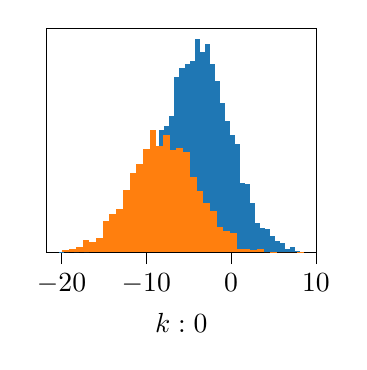
\begin{tikzpicture}

\definecolor{darkgray176}{RGB}{176,176,176}
\definecolor{darkorange25512714}{RGB}{255,127,14}
\definecolor{steelblue31119180}{RGB}{31,119,180}

\begin{axis}[
tick align=outside,
tick pos=left,
x grid style={darkgray176},
xlabel={$k: 0$},
xmin=-21.7817629577121, xmax=10.0412651951797,
xtick style={color=black},
y grid style={darkgray176},
%ylabel={Frequency},
ymin=0, ymax=369.6,
%ytick style={color=black},
ytick=\empty,
scale=0.5
]
\draw[draw=none,fill=steelblue31119180] (axis cs:-20.3352616780352,0) rectangle (axis cs:-19.7415116521512,1);
\draw[draw=none,fill=steelblue31119180] (axis cs:-19.7415116521512,0) rectangle (axis cs:-19.1477616262672,0);
\draw[draw=none,fill=steelblue31119180] (axis cs:-19.1477616262672,0) rectangle (axis cs:-18.5540116003831,3);
\draw[draw=none,fill=steelblue31119180] (axis cs:-18.5540116003831,0) rectangle (axis cs:-17.9602615744991,0);
\draw[draw=none,fill=steelblue31119180] (axis cs:-17.9602615744991,0) rectangle (axis cs:-17.3665115486151,2);
\draw[draw=none,fill=steelblue31119180] (axis cs:-17.3665115486151,0) rectangle (axis cs:-16.7727615227311,0);
\draw[draw=none,fill=steelblue31119180] (axis cs:-16.7727615227311,0) rectangle (axis cs:-16.179011496847,4);
\draw[draw=none,fill=steelblue31119180] (axis cs:-16.1790114968471,0) rectangle (axis cs:-15.585261470963,3);
\draw[draw=none,fill=steelblue31119180] (axis cs:-15.585261470963,0) rectangle (axis cs:-14.991511445079,6);
\draw[draw=none,fill=steelblue31119180] (axis cs:-14.991511445079,0) rectangle (axis cs:-14.397761419195,13);
\draw[draw=none,fill=steelblue31119180] (axis cs:-14.397761419195,0) rectangle (axis cs:-13.804011393311,17);
\draw[draw=none,fill=steelblue31119180] (axis cs:-13.804011393311,0) rectangle (axis cs:-13.2102613674269,18);
\draw[draw=none,fill=steelblue31119180] (axis cs:-13.2102613674269,0) rectangle (axis cs:-12.6165113415429,30);
\draw[draw=none,fill=steelblue31119180] (axis cs:-12.6165113415429,0) rectangle (axis cs:-12.0227613156589,43);
\draw[draw=none,fill=steelblue31119180] (axis cs:-12.0227613156589,0) rectangle (axis cs:-11.4290112897749,55);
\draw[draw=none,fill=steelblue31119180] (axis cs:-11.4290112897749,0) rectangle (axis cs:-10.8352612638908,70);
\draw[draw=none,fill=steelblue31119180] (axis cs:-10.8352612638908,0) rectangle (axis cs:-10.2415112380068,102);
\draw[draw=none,fill=steelblue31119180] (axis cs:-10.2415112380068,0) rectangle (axis cs:-9.64776121212279,111);
\draw[draw=none,fill=steelblue31119180] (axis cs:-9.64776121212279,0) rectangle (axis cs:-9.05401118623877,140);
\draw[draw=none,fill=steelblue31119180] (axis cs:-9.05401118623877,0) rectangle (axis cs:-8.46026116035475,161);
\draw[draw=none,fill=steelblue31119180] (axis cs:-8.46026116035475,0) rectangle (axis cs:-7.86651113447072,201);
\draw[draw=none,fill=steelblue31119180] (axis cs:-7.86651113447072,0) rectangle (axis cs:-7.2727611085867,209);
\draw[draw=none,fill=steelblue31119180] (axis cs:-7.2727611085867,0) rectangle (axis cs:-6.67901108270267,225);
\draw[draw=none,fill=steelblue31119180] (axis cs:-6.67901108270267,0) rectangle (axis cs:-6.08526105681865,290);
\draw[draw=none,fill=steelblue31119180] (axis cs:-6.08526105681865,0) rectangle (axis cs:-5.49151103093463,304);
\draw[draw=none,fill=steelblue31119180] (axis cs:-5.49151103093463,0) rectangle (axis cs:-4.8977610050506,311);
\draw[draw=none,fill=steelblue31119180] (axis cs:-4.8977610050506,0) rectangle (axis cs:-4.30401097916658,315);
\draw[draw=none,fill=steelblue31119180] (axis cs:-4.30401097916658,0) rectangle (axis cs:-3.71026095328256,352);
\draw[draw=none,fill=steelblue31119180] (axis cs:-3.71026095328256,0) rectangle (axis cs:-3.11651092739853,330);
\draw[draw=none,fill=steelblue31119180] (axis cs:-3.11651092739853,0) rectangle (axis cs:-2.52276090151451,343);
\draw[draw=none,fill=steelblue31119180] (axis cs:-2.52276090151451,0) rectangle (axis cs:-1.92901087563049,310);
\draw[draw=none,fill=steelblue31119180] (axis cs:-1.92901087563049,0) rectangle (axis cs:-1.33526084974646,282);
\draw[draw=none,fill=steelblue31119180] (axis cs:-1.33526084974646,0) rectangle (axis cs:-0.741510823862438,247);
\draw[draw=none,fill=steelblue31119180] (axis cs:-0.741510823862438,0) rectangle (axis cs:-0.147760797978414,217);
\draw[draw=none,fill=steelblue31119180] (axis cs:-0.147760797978414,0) rectangle (axis cs:0.44598922790561,193);
\draw[draw=none,fill=steelblue31119180] (axis cs:0.44598922790561,0) rectangle (axis cs:1.03973925378963,179);
\draw[draw=none,fill=steelblue31119180] (axis cs:1.03973925378963,0) rectangle (axis cs:1.63348927967366,114);
\draw[draw=none,fill=steelblue31119180] (axis cs:1.63348927967366,0) rectangle (axis cs:2.22723930555768,112);
\draw[draw=none,fill=steelblue31119180] (axis cs:2.22723930555768,0) rectangle (axis cs:2.82098933144171,81);
\draw[draw=none,fill=steelblue31119180] (axis cs:2.82098933144171,0) rectangle (axis cs:3.41473935732573,49);
\draw[draw=none,fill=steelblue31119180] (axis cs:3.41473935732573,0) rectangle (axis cs:4.00848938320975,41);
\draw[draw=none,fill=steelblue31119180] (axis cs:4.00848938320975,0) rectangle (axis cs:4.60223940909378,38);
\draw[draw=none,fill=steelblue31119180] (axis cs:4.60223940909378,0) rectangle (axis cs:5.1959894349778,27);
\draw[draw=none,fill=steelblue31119180] (axis cs:5.1959894349778,0) rectangle (axis cs:5.78973946086182,18);
\draw[draw=none,fill=steelblue31119180] (axis cs:5.78973946086182,0) rectangle (axis cs:6.38348948674585,15);
\draw[draw=none,fill=steelblue31119180] (axis cs:6.38348948674585,0) rectangle (axis cs:6.97723951262987,6);
\draw[draw=none,fill=steelblue31119180] (axis cs:6.97723951262987,0) rectangle (axis cs:7.5709895385139,9);
\draw[draw=none,fill=steelblue31119180] (axis cs:7.5709895385139,0) rectangle (axis cs:8.16473956439792,3);
\draw[draw=none,fill=darkorange25512714] (axis cs:-19.8926246009193,0) rectangle (axis cs:-19.1013082532409,4);
\draw[draw=none,fill=darkorange25512714] (axis cs:-19.1013082532409,0) rectangle (axis cs:-18.3099919055625,6);
\draw[draw=none,fill=darkorange25512714] (axis cs:-18.3099919055625,0) rectangle (axis cs:-17.5186755578841,9);
\draw[draw=none,fill=darkorange25512714] (axis cs:-17.5186755578841,0) rectangle (axis cs:-16.7273592102057,20);
\draw[draw=none,fill=darkorange25512714] (axis cs:-16.7273592102057,0) rectangle (axis cs:-15.9360428625273,17);
\draw[draw=none,fill=darkorange25512714] (axis cs:-15.9360428625273,0) rectangle (axis cs:-15.1447265148489,23);
\draw[draw=none,fill=darkorange25512714] (axis cs:-15.1447265148489,0) rectangle (axis cs:-14.3534101671705,51);
\draw[draw=none,fill=darkorange25512714] (axis cs:-14.3534101671705,0) rectangle (axis cs:-13.5620938194922,63);
\draw[draw=none,fill=darkorange25512714] (axis cs:-13.5620938194922,0) rectangle (axis cs:-12.7707774718138,72);
\draw[draw=none,fill=darkorange25512714] (axis cs:-12.7707774718138,0) rectangle (axis cs:-11.9794611241354,103);
\draw[draw=none,fill=darkorange25512714] (axis cs:-11.9794611241354,0) rectangle (axis cs:-11.188144776457,131);
\draw[draw=none,fill=darkorange25512714] (axis cs:-11.188144776457,0) rectangle (axis cs:-10.3968284287786,146);
\draw[draw=none,fill=darkorange25512714] (axis cs:-10.3968284287786,0) rectangle (axis cs:-9.6055120811002,170);
\draw[draw=none,fill=darkorange25512714] (axis cs:-9.6055120811002,0) rectangle (axis cs:-8.8141957334218,202);
\draw[draw=none,fill=darkorange25512714] (axis cs:-8.8141957334218,0) rectangle (axis cs:-8.02287938574342,176);
\draw[draw=none,fill=darkorange25512714] (axis cs:-8.02287938574341,0) rectangle (axis cs:-7.23156303806502,193);
\draw[draw=none,fill=darkorange25512714] (axis cs:-7.23156303806502,0) rectangle (axis cs:-6.44024669038663,168);
\draw[draw=none,fill=darkorange25512714] (axis cs:-6.44024669038663,0) rectangle (axis cs:-5.64893034270824,172);
\draw[draw=none,fill=darkorange25512714] (axis cs:-5.64893034270824,0) rectangle (axis cs:-4.85761399502985,166);
\draw[draw=none,fill=darkorange25512714] (axis cs:-4.85761399502985,0) rectangle (axis cs:-4.06629764735146,125);
\draw[draw=none,fill=darkorange25512714] (axis cs:-4.06629764735146,0) rectangle (axis cs:-3.27498129967307,102);
\draw[draw=none,fill=darkorange25512714] (axis cs:-3.27498129967307,0) rectangle (axis cs:-2.48366495199467,81);
\draw[draw=none,fill=darkorange25512714] (axis cs:-2.48366495199467,0) rectangle (axis cs:-1.69234860431628,68);
\draw[draw=none,fill=darkorange25512714] (axis cs:-1.69234860431628,0) rectangle (axis cs:-0.90103225663789,42);
\draw[draw=none,fill=darkorange25512714] (axis cs:-0.90103225663789,0) rectangle (axis cs:-0.109715908959497,36);
\draw[draw=none,fill=darkorange25512714] (axis cs:-0.109715908959497,0) rectangle (axis cs:0.681600438718892,32);
\draw[draw=none,fill=darkorange25512714] (axis cs:0.681600438718892,0) rectangle (axis cs:1.47291678639728,5);
\draw[draw=none,fill=darkorange25512714] (axis cs:1.47291678639728,0) rectangle (axis cs:2.26423313407568,6);
\draw[draw=none,fill=darkorange25512714] (axis cs:2.26423313407568,0) rectangle (axis cs:3.05554948175407,4);
\draw[draw=none,fill=darkorange25512714] (axis cs:3.05554948175407,0) rectangle (axis cs:3.84686582943246,5);
\draw[draw=none,fill=darkorange25512714] (axis cs:3.84686582943246,0) rectangle (axis cs:4.63818217711085,0);
\draw[draw=none,fill=darkorange25512714] (axis cs:4.63818217711085,0) rectangle (axis cs:5.42949852478924,1);
\draw[draw=none,fill=darkorange25512714] (axis cs:5.42949852478924,0) rectangle (axis cs:6.22081487246763,0);
\draw[draw=none,fill=darkorange25512714] (axis cs:6.22081487246763,0) rectangle (axis cs:7.01213122014602,0);
\draw[draw=none,fill=darkorange25512714] (axis cs:7.01213122014602,0) rectangle (axis cs:7.80344756782442,0);
\draw[draw=none,fill=darkorange25512714] (axis cs:7.80344756782442,0) rectangle (axis cs:8.59476391550281,1);
\end{axis}

\end{tikzpicture}

			%\caption{Caption for first figure}
			\label{fig:1}
		\end{minipage}
		\hfill
		\begin{minipage}[htbp]{0.24\textwidth}
			\centering
			% This file was created with tikzplotlib v0.10.1.
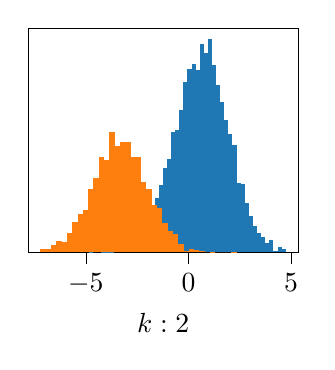
\begin{tikzpicture}

\definecolor{darkgray176}{RGB}{176,176,176}
\definecolor{darkorange25512714}{RGB}{255,127,14}
\definecolor{steelblue31119180}{RGB}{31,119,180}

\begin{axis}[
tick align=outside,
tick pos=left,
x grid style={darkgray176},
xlabel={$k:2$},
xmin=-7.80759693559219, xmax=5.34034850098321,
xtick style={color=black},
y grid style={darkgray176},
%ylabel={Frequency},
ymin=0, ymax=372.75,
%ytick style={color=black},
ytick=\empty,
scale=0.5
]
\draw[draw=none,fill=steelblue31119180] (axis cs:-4.84564394215464,0) rectangle (axis cs:-4.64588647216178,1);
\draw[draw=none,fill=steelblue31119180] (axis cs:-4.64588647216178,0) rectangle (axis cs:-4.44612900216892,0);
\draw[draw=none,fill=steelblue31119180] (axis cs:-4.44612900216892,0) rectangle (axis cs:-4.24637153217607,2);
\draw[draw=none,fill=steelblue31119180] (axis cs:-4.24637153217607,0) rectangle (axis cs:-4.04661406218321,1);
\draw[draw=none,fill=steelblue31119180] (axis cs:-4.04661406218321,0) rectangle (axis cs:-3.84685659219035,1);
\draw[draw=none,fill=steelblue31119180] (axis cs:-3.84685659219035,0) rectangle (axis cs:-3.64709912219749,1);
\draw[draw=none,fill=steelblue31119180] (axis cs:-3.64709912219749,0) rectangle (axis cs:-3.44734165220464,3);
\draw[draw=none,fill=steelblue31119180] (axis cs:-3.44734165220464,0) rectangle (axis cs:-3.24758418221178,4);
\draw[draw=none,fill=steelblue31119180] (axis cs:-3.24758418221178,0) rectangle (axis cs:-3.04782671221892,5);
\draw[draw=none,fill=steelblue31119180] (axis cs:-3.04782671221892,0) rectangle (axis cs:-2.84806924222607,9);
\draw[draw=none,fill=steelblue31119180] (axis cs:-2.84806924222606,0) rectangle (axis cs:-2.64831177223321,17);
\draw[draw=none,fill=steelblue31119180] (axis cs:-2.64831177223321,0) rectangle (axis cs:-2.44855430224035,25);
\draw[draw=none,fill=steelblue31119180] (axis cs:-2.44855430224035,0) rectangle (axis cs:-2.24879683224749,25);
\draw[draw=none,fill=steelblue31119180] (axis cs:-2.24879683224749,0) rectangle (axis cs:-2.04903936225464,41);
\draw[draw=none,fill=steelblue31119180] (axis cs:-2.04903936225464,0) rectangle (axis cs:-1.84928189226178,55);
\draw[draw=none,fill=steelblue31119180] (axis cs:-1.84928189226178,0) rectangle (axis cs:-1.64952442226892,70);
\draw[draw=none,fill=steelblue31119180] (axis cs:-1.64952442226892,0) rectangle (axis cs:-1.44976695227606,91);
\draw[draw=none,fill=steelblue31119180] (axis cs:-1.44976695227606,0) rectangle (axis cs:-1.25000948228321,112);
\draw[draw=none,fill=steelblue31119180] (axis cs:-1.25000948228321,0) rectangle (axis cs:-1.05025201229035,141);
\draw[draw=none,fill=steelblue31119180] (axis cs:-1.05025201229035,0) rectangle (axis cs:-0.850494542297493,156);
\draw[draw=none,fill=steelblue31119180] (axis cs:-0.850494542297493,0) rectangle (axis cs:-0.650737072304636,200);
\draw[draw=none,fill=steelblue31119180] (axis cs:-0.650737072304636,0) rectangle (axis cs:-0.450979602311778,203);
\draw[draw=none,fill=steelblue31119180] (axis cs:-0.450979602311778,0) rectangle (axis cs:-0.251222132318921,237);
\draw[draw=none,fill=steelblue31119180] (axis cs:-0.251222132318921,0) rectangle (axis cs:-0.0514646623260635,283);
\draw[draw=none,fill=steelblue31119180] (axis cs:-0.0514646623260635,0) rectangle (axis cs:0.148292807666794,305);
\draw[draw=none,fill=steelblue31119180] (axis cs:0.148292807666794,0) rectangle (axis cs:0.348050277659651,313);
\draw[draw=none,fill=steelblue31119180] (axis cs:0.348050277659651,0) rectangle (axis cs:0.547807747652509,303);
\draw[draw=none,fill=steelblue31119180] (axis cs:0.547807747652509,0) rectangle (axis cs:0.747565217645366,346);
\draw[draw=none,fill=steelblue31119180] (axis cs:0.747565217645366,0) rectangle (axis cs:0.947322687638223,332);
\draw[draw=none,fill=steelblue31119180] (axis cs:0.947322687638223,0) rectangle (axis cs:1.14708015763108,355);
\draw[draw=none,fill=steelblue31119180] (axis cs:1.14708015763108,0) rectangle (axis cs:1.34683762762394,312);
\draw[draw=none,fill=steelblue31119180] (axis cs:1.34683762762394,0) rectangle (axis cs:1.54659509761679,279);
\draw[draw=none,fill=steelblue31119180] (axis cs:1.54659509761679,0) rectangle (axis cs:1.74635256760965,250);
\draw[draw=none,fill=steelblue31119180] (axis cs:1.74635256760965,0) rectangle (axis cs:1.94611003760251,220);
\draw[draw=none,fill=steelblue31119180] (axis cs:1.94611003760251,0) rectangle (axis cs:2.14586750759537,197);
\draw[draw=none,fill=steelblue31119180] (axis cs:2.14586750759537,0) rectangle (axis cs:2.34562497758822,178);
\draw[draw=none,fill=steelblue31119180] (axis cs:2.34562497758822,0) rectangle (axis cs:2.54538244758108,115);
\draw[draw=none,fill=steelblue31119180] (axis cs:2.54538244758108,0) rectangle (axis cs:2.74513991757394,114);
\draw[draw=none,fill=steelblue31119180] (axis cs:2.74513991757394,0) rectangle (axis cs:2.9448973875668,82);
\draw[draw=none,fill=steelblue31119180] (axis cs:2.9448973875668,0) rectangle (axis cs:3.14465485755965,60);
\draw[draw=none,fill=steelblue31119180] (axis cs:3.14465485755965,0) rectangle (axis cs:3.34441232755251,44);
\draw[draw=none,fill=steelblue31119180] (axis cs:3.34441232755251,0) rectangle (axis cs:3.54416979754537,33);
\draw[draw=none,fill=steelblue31119180] (axis cs:3.54416979754537,0) rectangle (axis cs:3.74392726753822,26);
\draw[draw=none,fill=steelblue31119180] (axis cs:3.74392726753822,0) rectangle (axis cs:3.94368473753108,16);
\draw[draw=none,fill=steelblue31119180] (axis cs:3.94368473753108,0) rectangle (axis cs:4.14344220752394,21);
\draw[draw=none,fill=steelblue31119180] (axis cs:4.14344220752394,0) rectangle (axis cs:4.3431996775168,2);
\draw[draw=none,fill=steelblue31119180] (axis cs:4.3431996775168,0) rectangle (axis cs:4.54295714750965,9);
\draw[draw=none,fill=steelblue31119180] (axis cs:4.54295714750965,0) rectangle (axis cs:4.74271461750251,5);
\draw[draw=none,fill=darkorange25512714] (axis cs:-7.20996305211149,0) rectangle (axis cs:-6.95182942179264,6);
\draw[draw=none,fill=darkorange25512714] (axis cs:-6.95182942179264,0) rectangle (axis cs:-6.69369579147378,6);
\draw[draw=none,fill=darkorange25512714] (axis cs:-6.69369579147378,0) rectangle (axis cs:-6.43556216115493,12);
\draw[draw=none,fill=darkorange25512714] (axis cs:-6.43556216115493,0) rectangle (axis cs:-6.17742853083608,19);
\draw[draw=none,fill=darkorange25512714] (axis cs:-6.17742853083608,0) rectangle (axis cs:-5.91929490051723,18);
\draw[draw=none,fill=darkorange25512714] (axis cs:-5.91929490051722,0) rectangle (axis cs:-5.66116127019837,32);
\draw[draw=none,fill=darkorange25512714] (axis cs:-5.66116127019837,0) rectangle (axis cs:-5.40302763987952,50);
\draw[draw=none,fill=darkorange25512714] (axis cs:-5.40302763987952,0) rectangle (axis cs:-5.14489400956067,63);
\draw[draw=none,fill=darkorange25512714] (axis cs:-5.14489400956067,0) rectangle (axis cs:-4.88676037924181,71);
\draw[draw=none,fill=darkorange25512714] (axis cs:-4.88676037924181,0) rectangle (axis cs:-4.62862674892296,106);
\draw[draw=none,fill=darkorange25512714] (axis cs:-4.62862674892296,0) rectangle (axis cs:-4.37049311860411,123);
\draw[draw=none,fill=darkorange25512714] (axis cs:-4.37049311860411,0) rectangle (axis cs:-4.11235948828526,159);
\draw[draw=none,fill=darkorange25512714] (axis cs:-4.11235948828526,0) rectangle (axis cs:-3.8542258579664,153);
\draw[draw=none,fill=darkorange25512714] (axis cs:-3.8542258579664,0) rectangle (axis cs:-3.59609222764755,200);
\draw[draw=none,fill=darkorange25512714] (axis cs:-3.59609222764755,0) rectangle (axis cs:-3.3379585973287,177);
\draw[draw=none,fill=darkorange25512714] (axis cs:-3.3379585973287,0) rectangle (axis cs:-3.07982496700985,184);
\draw[draw=none,fill=darkorange25512714] (axis cs:-3.07982496700985,0) rectangle (axis cs:-2.82169133669099,184);
\draw[draw=none,fill=darkorange25512714] (axis cs:-2.82169133669099,0) rectangle (axis cs:-2.56355770637214,158);
\draw[draw=none,fill=darkorange25512714] (axis cs:-2.56355770637214,0) rectangle (axis cs:-2.30542407605329,159);
\draw[draw=none,fill=darkorange25512714] (axis cs:-2.30542407605329,0) rectangle (axis cs:-2.04729044573444,117);
\draw[draw=none,fill=darkorange25512714] (axis cs:-2.04729044573444,0) rectangle (axis cs:-1.78915681541558,105);
\draw[draw=none,fill=darkorange25512714] (axis cs:-1.78915681541558,0) rectangle (axis cs:-1.53102318509673,79);
\draw[draw=none,fill=darkorange25512714] (axis cs:-1.53102318509673,0) rectangle (axis cs:-1.27288955477788,73);
\draw[draw=none,fill=darkorange25512714] (axis cs:-1.27288955477788,0) rectangle (axis cs:-1.01475592445902,49);
\draw[draw=none,fill=darkorange25512714] (axis cs:-1.01475592445902,0) rectangle (axis cs:-0.756622294140172,36);
\draw[draw=none,fill=darkorange25512714] (axis cs:-0.756622294140172,0) rectangle (axis cs:-0.498488663821319,30);
\draw[draw=none,fill=darkorange25512714] (axis cs:-0.498488663821319,0) rectangle (axis cs:-0.240355033502467,14);
\draw[draw=none,fill=darkorange25512714] (axis cs:-0.240355033502467,0) rectangle (axis cs:0.0177785968163864,2);
\draw[draw=none,fill=darkorange25512714] (axis cs:0.0177785968163864,0) rectangle (axis cs:0.275912227135239,6);
\draw[draw=none,fill=darkorange25512714] (axis cs:0.275912227135239,0) rectangle (axis cs:0.534045857454092,4);
\draw[draw=none,fill=darkorange25512714] (axis cs:0.534045857454092,0) rectangle (axis cs:0.792179487772945,3);
\draw[draw=none,fill=darkorange25512714] (axis cs:0.792179487772945,0) rectangle (axis cs:1.0503131180918,0);
\draw[draw=none,fill=darkorange25512714] (axis cs:1.0503131180918,0) rectangle (axis cs:1.30844674841065,1);
\draw[draw=none,fill=darkorange25512714] (axis cs:1.30844674841065,0) rectangle (axis cs:1.5665803787295,0);
\draw[draw=none,fill=darkorange25512714] (axis cs:1.5665803787295,0) rectangle (axis cs:1.82471400904836,0);
\draw[draw=none,fill=darkorange25512714] (axis cs:1.82471400904836,0) rectangle (axis cs:2.08284763936721,0);
\draw[draw=none,fill=darkorange25512714] (axis cs:2.08284763936721,0) rectangle (axis cs:2.34098126968606,1);
\end{axis}

\end{tikzpicture}

			%\caption{Caption for second figure}
			\label{fig:2}
		\end{minipage}
		\hfill
		\begin{minipage}[htbp]{0.24\textwidth}
			\centering
			% This file was created with tikzplotlib v0.10.1.
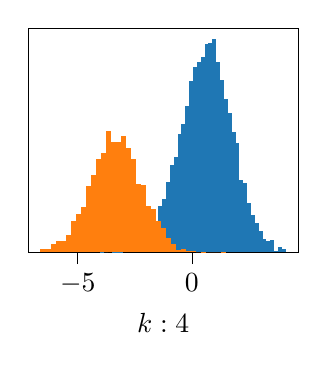
\begin{tikzpicture}

\definecolor{darkgray176}{RGB}{176,176,176}
\definecolor{darkorange25512714}{RGB}{255,127,14}
\definecolor{steelblue31119180}{RGB}{31,119,180}

\begin{axis}[
tick align=outside,
tick pos=left,
x grid style={darkgray176},
xlabel={$k:4$},
xmin=-7.16782843068525, xmax=4.65202446892355,
xtick style={color=black},
y grid style={darkgray176},
%ylabel={Frequency},
ymin=0, ymax=364.35,
%ytick style={color=black},
ytick=\empty,
scale=0.5
]
\draw[draw=none,fill=steelblue31119180] (axis cs:-4.01511339680388,0) rectangle (axis cs:-3.8457410671198,1);
\draw[draw=none,fill=steelblue31119180] (axis cs:-3.8457410671198,0) rectangle (axis cs:-3.67636873743571,0);
\draw[draw=none,fill=steelblue31119180] (axis cs:-3.67636873743571,0) rectangle (axis cs:-3.50699640775163,2);
\draw[draw=none,fill=steelblue31119180] (axis cs:-3.50699640775163,0) rectangle (axis cs:-3.33762407806754,1);
\draw[draw=none,fill=steelblue31119180] (axis cs:-3.33762407806754,0) rectangle (axis cs:-3.16825174838345,1);
\draw[draw=none,fill=steelblue31119180] (axis cs:-3.16825174838345,0) rectangle (axis cs:-2.99887941869937,1);
\draw[draw=none,fill=steelblue31119180] (axis cs:-2.99887941869937,0) rectangle (axis cs:-2.82950708901528,3);
\draw[draw=none,fill=steelblue31119180] (axis cs:-2.82950708901528,0) rectangle (axis cs:-2.6601347593312,4);
\draw[draw=none,fill=steelblue31119180] (axis cs:-2.6601347593312,0) rectangle (axis cs:-2.49076242964711,4);
\draw[draw=none,fill=steelblue31119180] (axis cs:-2.49076242964711,0) rectangle (axis cs:-2.32139009996302,8);
\draw[draw=none,fill=steelblue31119180] (axis cs:-2.32139009996302,0) rectangle (axis cs:-2.15201777027894,17);
\draw[draw=none,fill=steelblue31119180] (axis cs:-2.15201777027894,0) rectangle (axis cs:-1.98264544059485,27);
\draw[draw=none,fill=steelblue31119180] (axis cs:-1.98264544059485,0) rectangle (axis cs:-1.81327311091077,22);
\draw[draw=none,fill=steelblue31119180] (axis cs:-1.81327311091077,0) rectangle (axis cs:-1.64390078122668,43);
\draw[draw=none,fill=steelblue31119180] (axis cs:-1.64390078122668,0) rectangle (axis cs:-1.47452845154259,51);
\draw[draw=none,fill=steelblue31119180] (axis cs:-1.47452845154259,0) rectangle (axis cs:-1.30515612185851,76);
\draw[draw=none,fill=steelblue31119180] (axis cs:-1.30515612185851,0) rectangle (axis cs:-1.13578379217442,87);
\draw[draw=none,fill=steelblue31119180] (axis cs:-1.13578379217442,0) rectangle (axis cs:-0.966411462490336,114);
\draw[draw=none,fill=steelblue31119180] (axis cs:-0.966411462490336,0) rectangle (axis cs:-0.797039132806249,142);
\draw[draw=none,fill=steelblue31119180] (axis cs:-0.797039132806249,0) rectangle (axis cs:-0.627666803122163,155);
\draw[draw=none,fill=steelblue31119180] (axis cs:-0.627666803122163,0) rectangle (axis cs:-0.458294473438078,192);
\draw[draw=none,fill=steelblue31119180] (axis cs:-0.458294473438078,0) rectangle (axis cs:-0.288922143753991,208);
\draw[draw=none,fill=steelblue31119180] (axis cs:-0.288922143753991,0) rectangle (axis cs:-0.119549814069905,238);
\draw[draw=none,fill=steelblue31119180] (axis cs:-0.119549814069905,0) rectangle (axis cs:0.0498225156141805,278);
\draw[draw=none,fill=steelblue31119180] (axis cs:0.0498225156141805,0) rectangle (axis cs:0.219194845298267,302);
\draw[draw=none,fill=steelblue31119180] (axis cs:0.219194845298267,0) rectangle (axis cs:0.388567174982352,310);
\draw[draw=none,fill=steelblue31119180] (axis cs:0.388567174982352,0) rectangle (axis cs:0.557939504666439,317);
\draw[draw=none,fill=steelblue31119180] (axis cs:0.557939504666439,0) rectangle (axis cs:0.727311834350525,339);
\draw[draw=none,fill=steelblue31119180] (axis cs:0.727311834350525,0) rectangle (axis cs:0.89668416403461,341);
\draw[draw=none,fill=steelblue31119180] (axis cs:0.89668416403461,0) rectangle (axis cs:1.0660564937187,347);
\draw[draw=none,fill=steelblue31119180] (axis cs:1.0660564937187,0) rectangle (axis cs:1.23542882340278,310);
\draw[draw=none,fill=steelblue31119180] (axis cs:1.23542882340278,0) rectangle (axis cs:1.40480115308687,281);
\draw[draw=none,fill=steelblue31119180] (axis cs:1.40480115308687,0) rectangle (axis cs:1.57417348277095,249);
\draw[draw=none,fill=steelblue31119180] (axis cs:1.57417348277095,0) rectangle (axis cs:1.74354581245504,227);
\draw[draw=none,fill=steelblue31119180] (axis cs:1.74354581245504,0) rectangle (axis cs:1.91291814213913,195);
\draw[draw=none,fill=steelblue31119180] (axis cs:1.91291814213913,0) rectangle (axis cs:2.08229047182321,177);
\draw[draw=none,fill=steelblue31119180] (axis cs:2.08229047182321,0) rectangle (axis cs:2.2516628015073,117);
\draw[draw=none,fill=steelblue31119180] (axis cs:2.2516628015073,0) rectangle (axis cs:2.42103513119138,113);
\draw[draw=none,fill=steelblue31119180] (axis cs:2.42103513119138,0) rectangle (axis cs:2.59040746087547,81);
\draw[draw=none,fill=steelblue31119180] (axis cs:2.59040746087547,0) rectangle (axis cs:2.75977979055956,60);
\draw[draw=none,fill=steelblue31119180] (axis cs:2.75977979055956,0) rectangle (axis cs:2.92915212024364,47);
\draw[draw=none,fill=steelblue31119180] (axis cs:2.92915212024364,0) rectangle (axis cs:3.09852444992773,34);
\draw[draw=none,fill=steelblue31119180] (axis cs:3.09852444992773,0) rectangle (axis cs:3.26789677961181,22);
\draw[draw=none,fill=steelblue31119180] (axis cs:3.26789677961181,0) rectangle (axis cs:3.4372691092959,19);
\draw[draw=none,fill=steelblue31119180] (axis cs:3.4372691092959,0) rectangle (axis cs:3.60664143897999,20);
\draw[draw=none,fill=steelblue31119180] (axis cs:3.60664143897999,0) rectangle (axis cs:3.77601376866407,3);
\draw[draw=none,fill=steelblue31119180] (axis cs:3.77601376866407,0) rectangle (axis cs:3.94538609834816,8);
\draw[draw=none,fill=steelblue31119180] (axis cs:3.94538609834816,0) rectangle (axis cs:4.11475842803224,6);
\draw[draw=none,fill=darkorange25512714] (axis cs:-6.63056238979394,0) rectangle (axis cs:-6.41096241157501,6);
\draw[draw=none,fill=darkorange25512714] (axis cs:-6.41096241157501,0) rectangle (axis cs:-6.19136243335608,5);
\draw[draw=none,fill=darkorange25512714] (axis cs:-6.19136243335608,0) rectangle (axis cs:-5.97176245513715,14);
\draw[draw=none,fill=darkorange25512714] (axis cs:-5.97176245513715,0) rectangle (axis cs:-5.75216247691822,18);
\draw[draw=none,fill=darkorange25512714] (axis cs:-5.75216247691822,0) rectangle (axis cs:-5.53256249869928,18);
\draw[draw=none,fill=darkorange25512714] (axis cs:-5.53256249869928,0) rectangle (axis cs:-5.31296252048035,29);
\draw[draw=none,fill=darkorange25512714] (axis cs:-5.31296252048035,0) rectangle (axis cs:-5.09336254226142,51);
\draw[draw=none,fill=darkorange25512714] (axis cs:-5.09336254226142,0) rectangle (axis cs:-4.87376256404249,63);
\draw[draw=none,fill=darkorange25512714] (axis cs:-4.87376256404249,0) rectangle (axis cs:-4.65416258582356,73);
\draw[draw=none,fill=darkorange25512714] (axis cs:-4.65416258582356,0) rectangle (axis cs:-4.43456260760463,108);
\draw[draw=none,fill=darkorange25512714] (axis cs:-4.43456260760463,0) rectangle (axis cs:-4.2149626293857,125);
\draw[draw=none,fill=darkorange25512714] (axis cs:-4.2149626293857,0) rectangle (axis cs:-3.99536265116677,152);
\draw[draw=none,fill=darkorange25512714] (axis cs:-3.99536265116677,0) rectangle (axis cs:-3.77576267294784,161);
\draw[draw=none,fill=darkorange25512714] (axis cs:-3.77576267294784,0) rectangle (axis cs:-3.55616269472891,198);
\draw[draw=none,fill=darkorange25512714] (axis cs:-3.55616269472891,0) rectangle (axis cs:-3.33656271650998,179);
\draw[draw=none,fill=darkorange25512714] (axis cs:-3.33656271650998,0) rectangle (axis cs:-3.11696273829105,179);
\draw[draw=none,fill=darkorange25512714] (axis cs:-3.11696273829105,0) rectangle (axis cs:-2.89736276007212,189);
\draw[draw=none,fill=darkorange25512714] (axis cs:-2.89736276007212,0) rectangle (axis cs:-2.67776278185319,170);
\draw[draw=none,fill=darkorange25512714] (axis cs:-2.67776278185319,0) rectangle (axis cs:-2.45816280363426,151);
\draw[draw=none,fill=darkorange25512714] (axis cs:-2.45816280363426,0) rectangle (axis cs:-2.23856282541533,111);
\draw[draw=none,fill=darkorange25512714] (axis cs:-2.23856282541533,0) rectangle (axis cs:-2.01896284719639,109);
\draw[draw=none,fill=darkorange25512714] (axis cs:-2.01896284719639,0) rectangle (axis cs:-1.79936286897746,75);
\draw[draw=none,fill=darkorange25512714] (axis cs:-1.79936286897746,0) rectangle (axis cs:-1.57976289075853,71);
\draw[draw=none,fill=darkorange25512714] (axis cs:-1.57976289075853,0) rectangle (axis cs:-1.3601629125396,51);
\draw[draw=none,fill=darkorange25512714] (axis cs:-1.3601629125396,0) rectangle (axis cs:-1.14056293432067,40);
\draw[draw=none,fill=darkorange25512714] (axis cs:-1.14056293432067,0) rectangle (axis cs:-0.920962956101741,24);
\draw[draw=none,fill=darkorange25512714] (axis cs:-0.920962956101741,0) rectangle (axis cs:-0.701362977882811,13);
\draw[draw=none,fill=darkorange25512714] (axis cs:-0.701362977882811,0) rectangle (axis cs:-0.481762999663879,4);
\draw[draw=none,fill=darkorange25512714] (axis cs:-0.481762999663879,0) rectangle (axis cs:-0.262163021444949,5);
\draw[draw=none,fill=darkorange25512714] (axis cs:-0.262163021444949,0) rectangle (axis cs:-0.0425630432260187,3);
\draw[draw=none,fill=darkorange25512714] (axis cs:-0.0425630432260187,0) rectangle (axis cs:0.177036934992913,3);
\draw[draw=none,fill=darkorange25512714] (axis cs:0.177036934992913,0) rectangle (axis cs:0.396636913211843,0);
\draw[draw=none,fill=darkorange25512714] (axis cs:0.396636913211843,0) rectangle (axis cs:0.616236891430773,1);
\draw[draw=none,fill=darkorange25512714] (axis cs:0.616236891430773,0) rectangle (axis cs:0.835836869649705,0);
\draw[draw=none,fill=darkorange25512714] (axis cs:0.835836869649705,0) rectangle (axis cs:1.05543684786864,0);
\draw[draw=none,fill=darkorange25512714] (axis cs:1.05543684786864,0) rectangle (axis cs:1.27503682608757,0);
\draw[draw=none,fill=darkorange25512714] (axis cs:1.27503682608757,0) rectangle (axis cs:1.4946368043065,1);
\end{axis}

\end{tikzpicture}

			%\caption{Caption for third figure}
			\label{fig:3}
		\end{minipage}
		\hfill
		\begin{minipage}[htbp]{0.24\textwidth}
			\centering
			% This file was created with tikzplotlib v0.10.1.
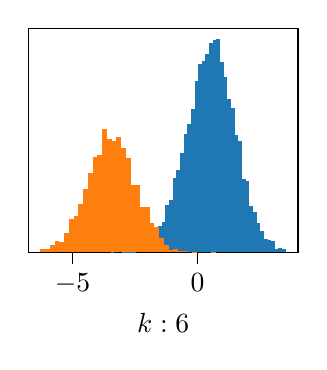
\begin{tikzpicture}

\definecolor{darkgray176}{RGB}{176,176,176}
\definecolor{darkorange25512714}{RGB}{255,127,14}
\definecolor{steelblue31119180}{RGB}{31,119,180}

\begin{axis}[
tick align=outside,
tick pos=left,
x grid style={darkgray176},
xlabel={$k:6$},
xmin=-6.77573066190925, xmax=4.02780843120382,
xtick style={color=black},
y grid style={darkgray176},
%ylabel={Frequency},
ymin=0, ymax=362.25,
ytick=\empty,
%ytick style={color=black},
scale=0.5
]
\draw[draw=none,fill=steelblue31119180] (axis cs:-3.4770362703687,0) rectangle (axis cs:-3.33091596322714,1);
\draw[draw=none,fill=steelblue31119180] (axis cs:-3.33091596322714,0) rectangle (axis cs:-3.18479565608559,0);
\draw[draw=none,fill=steelblue31119180] (axis cs:-3.18479565608559,0) rectangle (axis cs:-3.03867534894403,2);
\draw[draw=none,fill=steelblue31119180] (axis cs:-3.03867534894403,0) rectangle (axis cs:-2.89255504180248,1);
\draw[draw=none,fill=steelblue31119180] (axis cs:-2.89255504180248,0) rectangle (axis cs:-2.74643473466092,1);
\draw[draw=none,fill=steelblue31119180] (axis cs:-2.74643473466092,0) rectangle (axis cs:-2.60031442751937,1);
\draw[draw=none,fill=steelblue31119180] (axis cs:-2.60031442751937,0) rectangle (axis cs:-2.45419412037781,1);
\draw[draw=none,fill=steelblue31119180] (axis cs:-2.45419412037781,0) rectangle (axis cs:-2.30807381323626,5);
\draw[draw=none,fill=steelblue31119180] (axis cs:-2.30807381323626,0) rectangle (axis cs:-2.1619535060947,5);
\draw[draw=none,fill=steelblue31119180] (axis cs:-2.1619535060947,0) rectangle (axis cs:-2.01583319895314,7);
\draw[draw=none,fill=steelblue31119180] (axis cs:-2.01583319895315,0) rectangle (axis cs:-1.86971289181159,16);
\draw[draw=none,fill=steelblue31119180] (axis cs:-1.86971289181159,0) rectangle (axis cs:-1.72359258467004,27);
\draw[draw=none,fill=steelblue31119180] (axis cs:-1.72359258467004,0) rectangle (axis cs:-1.57747227752848,23);
\draw[draw=none,fill=steelblue31119180] (axis cs:-1.57747227752848,0) rectangle (axis cs:-1.43135197038692,43);
\draw[draw=none,fill=steelblue31119180] (axis cs:-1.43135197038692,0) rectangle (axis cs:-1.28523166324537,49);
\draw[draw=none,fill=steelblue31119180] (axis cs:-1.28523166324537,0) rectangle (axis cs:-1.13911135610381,77);
\draw[draw=none,fill=steelblue31119180] (axis cs:-1.13911135610381,0) rectangle (axis cs:-0.99299104896226,84);
\draw[draw=none,fill=steelblue31119180] (axis cs:-0.99299104896226,0) rectangle (axis cs:-0.846870741820704,120);
\draw[draw=none,fill=steelblue31119180] (axis cs:-0.846870741820704,0) rectangle (axis cs:-0.700750434679149,133);
\draw[draw=none,fill=steelblue31119180] (axis cs:-0.700750434679149,0) rectangle (axis cs:-0.554630127537594,160);
\draw[draw=none,fill=steelblue31119180] (axis cs:-0.554630127537594,0) rectangle (axis cs:-0.408509820396039,192);
\draw[draw=none,fill=steelblue31119180] (axis cs:-0.408509820396039,0) rectangle (axis cs:-0.262389513254484,207);
\draw[draw=none,fill=steelblue31119180] (axis cs:-0.262389513254484,0) rectangle (axis cs:-0.116269206112929,232);
\draw[draw=none,fill=steelblue31119180] (axis cs:-0.116269206112929,0) rectangle (axis cs:0.0298511010286262,277);
\draw[draw=none,fill=steelblue31119180] (axis cs:0.0298511010286262,0) rectangle (axis cs:0.175971408170181,304);
\draw[draw=none,fill=steelblue31119180] (axis cs:0.175971408170181,0) rectangle (axis cs:0.322091715311736,309);
\draw[draw=none,fill=steelblue31119180] (axis cs:0.322091715311736,0) rectangle (axis cs:0.468212022453292,321);
\draw[draw=none,fill=steelblue31119180] (axis cs:0.468212022453292,0) rectangle (axis cs:0.614332329594847,339);
\draw[draw=none,fill=steelblue31119180] (axis cs:0.614332329594847,0) rectangle (axis cs:0.760452636736401,344);
\draw[draw=none,fill=steelblue31119180] (axis cs:0.760452636736401,0) rectangle (axis cs:0.906572943877957,345);
\draw[draw=none,fill=steelblue31119180] (axis cs:0.906572943877957,0) rectangle (axis cs:1.05269325101951,307);
\draw[draw=none,fill=steelblue31119180] (axis cs:1.05269325101951,0) rectangle (axis cs:1.19881355816107,283);
\draw[draw=none,fill=steelblue31119180] (axis cs:1.19881355816107,0) rectangle (axis cs:1.34493386530262,248);
\draw[draw=none,fill=steelblue31119180] (axis cs:1.34493386530262,0) rectangle (axis cs:1.49105417244418,233);
\draw[draw=none,fill=steelblue31119180] (axis cs:1.49105417244418,0) rectangle (axis cs:1.63717447958573,189);
\draw[draw=none,fill=steelblue31119180] (axis cs:1.63717447958573,0) rectangle (axis cs:1.78329478672729,180);
\draw[draw=none,fill=steelblue31119180] (axis cs:1.78329478672729,0) rectangle (axis cs:1.92941509386884,118);
\draw[draw=none,fill=steelblue31119180] (axis cs:1.92941509386884,0) rectangle (axis cs:2.0755354010104,115);
\draw[draw=none,fill=steelblue31119180] (axis cs:2.0755354010104,0) rectangle (axis cs:2.22165570815195,75);
\draw[draw=none,fill=steelblue31119180] (axis cs:2.22165570815195,0) rectangle (axis cs:2.36777601529351,65);
\draw[draw=none,fill=steelblue31119180] (axis cs:2.36777601529351,0) rectangle (axis cs:2.51389632243506,48);
\draw[draw=none,fill=steelblue31119180] (axis cs:2.51389632243506,0) rectangle (axis cs:2.66001662957662,35);
\draw[draw=none,fill=steelblue31119180] (axis cs:2.66001662957662,0) rectangle (axis cs:2.80613693671817,22);
\draw[draw=none,fill=steelblue31119180] (axis cs:2.80613693671817,0) rectangle (axis cs:2.95225724385973,20);
\draw[draw=none,fill=steelblue31119180] (axis cs:2.95225724385973,0) rectangle (axis cs:3.09837755100128,18);
\draw[draw=none,fill=steelblue31119180] (axis cs:3.09837755100128,0) rectangle (axis cs:3.24449785814284,5);
\draw[draw=none,fill=steelblue31119180] (axis cs:3.24449785814284,0) rectangle (axis cs:3.39061816528439,7);
\draw[draw=none,fill=steelblue31119180] (axis cs:3.39061816528439,0) rectangle (axis cs:3.53673847242595,6);
\draw[draw=none,fill=darkorange25512714] (axis cs:-6.28466070313138,0) rectangle (axis cs:-6.09454834083815,6);
\draw[draw=none,fill=darkorange25512714] (axis cs:-6.09454834083815,0) rectangle (axis cs:-5.90443597854491,5);
\draw[draw=none,fill=darkorange25512714] (axis cs:-5.90443597854491,0) rectangle (axis cs:-5.71432361625168,12);
\draw[draw=none,fill=darkorange25512714] (axis cs:-5.71432361625168,0) rectangle (axis cs:-5.52421125395844,19);
\draw[draw=none,fill=darkorange25512714] (axis cs:-5.52421125395844,0) rectangle (axis cs:-5.33409889166521,17);
\draw[draw=none,fill=darkorange25512714] (axis cs:-5.33409889166521,0) rectangle (axis cs:-5.14398652937197,31);
\draw[draw=none,fill=darkorange25512714] (axis cs:-5.14398652937197,0) rectangle (axis cs:-4.95387416707874,54);
\draw[draw=none,fill=darkorange25512714] (axis cs:-4.95387416707874,0) rectangle (axis cs:-4.7637618047855,59);
\draw[draw=none,fill=darkorange25512714] (axis cs:-4.7637618047855,0) rectangle (axis cs:-4.57364944249227,78);
\draw[draw=none,fill=darkorange25512714] (axis cs:-4.57364944249227,0) rectangle (axis cs:-4.38353708019903,102);
\draw[draw=none,fill=darkorange25512714] (axis cs:-4.38353708019903,0) rectangle (axis cs:-4.1934247179058,128);
\draw[draw=none,fill=darkorange25512714] (axis cs:-4.1934247179058,0) rectangle (axis cs:-4.00331235561256,154);
\draw[draw=none,fill=darkorange25512714] (axis cs:-4.00331235561256,0) rectangle (axis cs:-3.81319999331933,158);
\draw[draw=none,fill=darkorange25512714] (axis cs:-3.81319999331933,0) rectangle (axis cs:-3.62308763102609,200);
\draw[draw=none,fill=darkorange25512714] (axis cs:-3.62308763102609,0) rectangle (axis cs:-3.43297526873286,183);
\draw[draw=none,fill=darkorange25512714] (axis cs:-3.43297526873286,0) rectangle (axis cs:-3.24286290643962,180);
\draw[draw=none,fill=darkorange25512714] (axis cs:-3.24286290643962,0) rectangle (axis cs:-3.05275054414639,186);
\draw[draw=none,fill=darkorange25512714] (axis cs:-3.05275054414639,0) rectangle (axis cs:-2.86263818185316,168);
\draw[draw=none,fill=darkorange25512714] (axis cs:-2.86263818185316,0) rectangle (axis cs:-2.67252581955992,153);
\draw[draw=none,fill=darkorange25512714] (axis cs:-2.67252581955992,0) rectangle (axis cs:-2.48241345726669,109);
\draw[draw=none,fill=darkorange25512714] (axis cs:-2.48241345726669,0) rectangle (axis cs:-2.29230109497345,109);
\draw[draw=none,fill=darkorange25512714] (axis cs:-2.29230109497345,0) rectangle (axis cs:-2.10218873268022,74);
\draw[draw=none,fill=darkorange25512714] (axis cs:-2.10218873268022,0) rectangle (axis cs:-1.91207637038698,74);
\draw[draw=none,fill=darkorange25512714] (axis cs:-1.91207637038698,0) rectangle (axis cs:-1.72196400809375,48);
\draw[draw=none,fill=darkorange25512714] (axis cs:-1.72196400809375,0) rectangle (axis cs:-1.53185164580051,41);
\draw[draw=none,fill=darkorange25512714] (axis cs:-1.53185164580051,0) rectangle (axis cs:-1.34173928350728,23);
\draw[draw=none,fill=darkorange25512714] (axis cs:-1.34173928350728,0) rectangle (axis cs:-1.15162692121404,12);
\draw[draw=none,fill=darkorange25512714] (axis cs:-1.15162692121404,0) rectangle (axis cs:-0.961514558920808,4);
\draw[draw=none,fill=darkorange25512714] (axis cs:-0.961514558920808,0) rectangle (axis cs:-0.771402196627573,6);
\draw[draw=none,fill=darkorange25512714] (axis cs:-0.771402196627573,0) rectangle (axis cs:-0.581289834334338,2);
\draw[draw=none,fill=darkorange25512714] (axis cs:-0.581289834334338,0) rectangle (axis cs:-0.391177472041103,3);
\draw[draw=none,fill=darkorange25512714] (axis cs:-0.391177472041103,0) rectangle (axis cs:-0.201065109747868,0);
\draw[draw=none,fill=darkorange25512714] (axis cs:-0.201065109747868,0) rectangle (axis cs:-0.0109527474546338,1);
\draw[draw=none,fill=darkorange25512714] (axis cs:-0.0109527474546338,0) rectangle (axis cs:0.179159614838601,0);
\draw[draw=none,fill=darkorange25512714] (axis cs:0.179159614838601,0) rectangle (axis cs:0.369271977131836,0);
\draw[draw=none,fill=darkorange25512714] (axis cs:0.369271977131836,0) rectangle (axis cs:0.559384339425071,0);
\draw[draw=none,fill=darkorange25512714] (axis cs:0.559384339425071,0) rectangle (axis cs:0.749496701718305,1);
\end{axis}

\end{tikzpicture}

			%\caption{Caption for fourth figure}
			\label{fig:4}
		\end{minipage}
		\caption{Residuals with respect to $\mathbb{P}$ and $\mathbb{Q}$, $k$ represents optimization step.}
		\label{fig:normal-residual}
	\end{figure}

	\subsection{Proof of Theorem~\ref{thm:improvement-of-theta}}
	\label{app:improvement-of-theta}
	\begin{proof}
		To show the change in $\varepsilon$ we will first calculate the expected change in $\vtheta$ by the $\vtheta$-update described in Equation \ref{eqn:theta-update}. We will also introduce some notation, $\mathcal{S}$ represents all $\vx \in X$ that are within the lowest $np$ losses, i.e. within the subquantile, $\vp \in \mathcal{S}$ represent all data vectors from $\mathbb{P}$ that are within the SubQuantile, similarly $\vq \in \mathbb{Q}$ represent all data vectors from $\mathbb{Q}$ that are within the SubQuantile. Furthermore, $|\mathcal{S}| = np$, there are $\varepsilon np$ points from $\mathbb{Q}$ in $\mathcal{S}$ and $(1-\varepsilon)np$ points from $\mathbb{P}$ within $\mathcal{S}$.  We assume $\vp \sim \mathcal{N}(\vzero, \Sigma_P)$ and $\vq \sim \mathcal{N}(\vzero, \Sigma_Q)$ where $\Sigma_P = \xi_P I$ and $\Sigma_Q = \xi_Q I$ where $\xi_P$ and $\xi_Q$ are greater than $0$, then we can assume it follows $\displaystyle \vmu\vmu^\top = \vzero\vzero^\top = 0$. 
		\begingroup
		%\addtolength{\jot}{0.5em}
		\begin{align*}
			\mathbb{E}\left[\vtheta_{k+1}\right] &= \vtheta_k - \mathbb{E}\left[\alpha \nabla g(\vtheta_k,t_{k+1})\right] &&\\
			&= \vtheta_k - \alpha \mathbb{E}\left[\sum_{\vx \in \mathcal{S}}\vx(\vtheta^\top\vx - y) \right] &&\\
			&= \vtheta_k - \alpha \mathbb{E}\left[\sum_{\vx \in \mathcal{S}}\vx\vx^\top\vtheta_k - \vx y \right] &&\\
			&= \vtheta_k - \alpha \mathbb{E}\left[\sum_{\vp \in \mathcal{S}}\vp\vp^\top\vtheta_k - \vp y_p + \sum_{\vq \in \mathcal{S}} \vq\vq^\top\vtheta_k - \vq y_q \right] &&
			\intertext{We will use Assumption \ref{asm:normal-corruption} to rewrite $y_p$ and $y_q$}
			&= \vtheta_k - \alpha \mathbb{E}\left[\sum_{\vp \in \mathcal{S}}\vp\vp^\top\vtheta_k - \vp (\vbeta_P \vp + \eps_P) + \sum_{\vq \in \mathcal{S}} \vq\vq^\top\vtheta_k - \vq (\vbeta_Q \vp + \eps_Q) \right] &&\\
			&= \vtheta_k - \alpha\left(\sum_{\vp \in \mathcal{S}} \left(\vmu \vmu^\top + \Sigma_P\right)\vtheta_k - \left(\vmu \vmu^\top + \Sigma_P\right)\vbeta_P + \sum_{\vq \in \mathcal{S}} \left(\vmu \vmu^\top + \Sigma_Q\right)\vtheta_k - \left(\vmu \vmu^\top + \Sigma_Q\right)\vbeta_Q\right) &&
		\end{align*}
		 \vspace{1em}
		\begin{equation}\vspace{1em}
			\mathbb{E}\left[\vtheta_{(t+1)}\right]= \vtheta_{(t)} - \alpha np \left( (1-\varepsilon^{(t)})\xi_P(\vtheta_{(t)} - \vbeta_P ) + \varepsilon^{(t)}\xi_Q(\vtheta_{(t)} - \vbeta_Q)\right) 
		\end{equation}
		
		\endgroup
		Now that we have the expected update for $\vtheta$ in terms of the linear regression coefficients, we now want to utilize Lemma \ref{lem:effect-of-projection}.\\
		Let $\displaystyle \vtheta_{(t)} = \alpha_1^{(t)}\vbeta_P + \alpha_2^{(t)}\vbeta_Q + \sum_{i=3}^{d}\alpha_i^{(t)} \vr_i$ in the same basis $\mB$ defined in Lemma \ref{lem:effect-of-projection}.Let $\gamma \triangleq \alpha np$. Then the following manipulations hold:
		\begin{align*}
			\mathbb{E}\left[\vtheta_{(t+1)}\right] &= \vtheta_{(t)} - \gamma \left( (1-\varepsilon^{(t)})\xi_P(\vtheta_{(t)} - \vbeta_P ) + \varepsilon^{(t)}\xi_Q(\vtheta_{(t)} - \vbeta_Q)\right) &&\\
			&= \vtheta_{(t)}\left(1 - \gamma\left(\left(1 - \varepsilon^{(t)}\right)\xi_P + \varepsilon^{(t)}\xi_Q\right)\right) + \gamma \left(1 - \varepsilon^{(t)}\right)\xi_P\vbeta_P + \gamma \varepsilon^{(t)} \xi_Q \vbeta_Q&&\\
			&= \left(1 - \gamma\left(\left(1 - \varepsilon^{(t)}\right)\xi_P + \varepsilon^{(t)}\xi_Q\right)\right)\left(\alpha_1^{(t)} \vbeta_P + \alpha_2^{(t)} \vbeta_Q + \sum_{i=3}^d\alpha_i^{(t)}\vr_i\right) + \gamma \left(1 - \varepsilon^{(t)}\right)\xi_P\vbeta_P + \gamma \varepsilon^{(t)} \xi_Q \vbeta_Q &&
		\end{align*}
		To simplify the notation, let us define the constant for this iteration $\displaystyle \Xi^{(t)} \triangleq \left(1 - \gamma\left(\left(1 - \varepsilon^{(t)}\right)\xi_P + \varepsilon^{(t)}\xi_Q\right)\right)$ 
		\begin{align*}
			&= \left(\alpha_1^{(t)}\Xi^{(t)} + \gamma\left(1-\varepsilon^{(t)}\right)\xi_P\right)\vbeta_P + \left(\alpha_2^{(t)}\Xi^{(t)} + \gamma \varepsilon^{(t)}\xi_Q\right)\vbeta_Q + \Xi^{(t)}\sum_{i=3}^d\alpha_i^{(t)}\vr_i &&
		\end{align*}
		We will now calculate the difference. 
		\begin{align*}
			\mathbb{E}\left[\vtheta_{(t+1)} - \vtheta_{(t)}\right] &= \left(\alpha_1^{(t)}\left(\Xi^{(t)}-1\right) + \gamma\left(1-\varepsilon^{(t)}\right)\xi_P\right)\vbeta_P + \left(\alpha_2^{(t)}\left(\Xi^{(t)}-1\right) + \gamma \varepsilon^{(t)}\xi_Q\right)\vbeta_Q + \left(\Xi^{(t)}-1\right)\sum_{i=3}^d\alpha_i^{(t)}\vr_i&&\\
		\end{align*}
		Thus the conditions for $\varepsilon$ to decrease by expectation are:
		\begin{equation}
			\norm{\left(\alpha_1^{(t)}\left(\Xi^{(t)}-1\right) + \gamma\left(1-\varepsilon^{(t)}\right)\xi_P\right)\vbeta_P} > \norm{\left(\alpha_2^{(t)}\left(\Xi^{(t)}-1\right) + \gamma \varepsilon^{(t)}\xi_Q\right)\vbeta_Q}
		\end{equation}  
		This concludes the proof. Note we are not interested in the change on the vectors $\vr_3, \dots, \vr_d$ as they do not have an effect on the projection of $\vtheta$ onto $\vbeta_P$ and $\vbeta_Q$. 
	\end{proof}

	\newpage
	
	\section{Proofs for Convergence}
	\label{app:convergence-proofs}
	\subsection{Proof of Theorem ~\ref{thm:convergence-guarantee}}
	\begin{proof}
	We will first start by introducing new notation. Let $S$ represent a matrix with $np$ data points from $X$, in other words it is a possible SubQuantile Matrix. Let $\displaystyle\vPi$ represent the set of all such possible matrices $S$ of $X$. Note $\displaystyle \left|\vPi\right| = \binom{n}{np}$. We can now redefine the min-max optimization problem of $g$ to a min-min optimization problem. Let us define the function $f(\vtheta, S) = \norm{\vtheta^\top S - y_S}_2^2$
	\begin{equation}
		\vtheta^*, S^* = \argmin_{\vtheta \in \mathbb{R}^d} \argmin_{S \in \vPi} \norm{\vtheta^\top S - y_S}_2^2
	\end{equation}
	Note we have a $\mathcal{O}(n)$ time-complexity oracle for the $\displaystyle \argmin_{S\in \vPi}f(\vtheta_T,S_T)$. 
	\begin{restatable}{lemma}{unique-S-minimizer}
		\label{lem:unique-S-minimizer}
		The resultant $\displaystyle \widetilde{S} = \argmin_{S \in \vPi} f(\vtheta,S)$ is a unique minimizer iff all points in $X$ are different. 
	\end{restatable}
	We will now show $f$ is a monotonically decreasing function.\\
	First let us define $\phi(\cdot) = \min_{S \in \vPi}\left(\cdot,S\right)$. 
	Let us also note $f$ is $\ell$ smooth with respect to $\vtheta$. This is following notation from \cite{Jin_2019}.It thus follows:
	\begin{align*}
		f(\vtheta_{k+1}, S_k) &\leq f(\vtheta_k, S_k) + \langle\nabla_\vtheta f(\vtheta_k,S_k), \vtheta_{k+1}-\vtheta_k \rangle + \frac{\ell}{2}\norm{\vtheta_{k+1}-\vtheta_k}_2^2 &&\\
		&= \phi(\vtheta_k) + \langle\nabla_\vtheta f(\vtheta_k,S_k), -\frac{1}{\ell}\nabla_\vtheta f(\vtheta_k,S_k)\rangle + \frac{\ell}{2}\norm{\frac{1}{\ell}\nabla_\vtheta f(\vtheta_k,S_k)}_2^2 &&\\
		&= \phi(\vtheta_k) - \frac{1}{\ell}\left(\nabla_\vtheta f(\vtheta_k,S_k)\right)^2 + \frac{1}{2\ell}\left(\nabla_\vtheta f(\vtheta_k,S_k)\right)^2 &&\\
		&= \phi(\vtheta_k) - \frac{1}{2\ell}\left(\nabla_\vtheta f(\vtheta_k,S_k)\right)^2 &&\\
	\end{align*} 
	Thus we have proved the inner optimization problem is monotonically decreasing. Since the outer minimization is strictly less than or equal to the result from the inner optimization, it follows after each two step optimization: 
	\begin{align*}
		\phi(\vtheta_{k+1}) \leq \phi(\vtheta_k)
	\end{align*}
	
	Since $f$ is lower bounded by $0$. We can invoke Montonicity Convergence Theorem, since $f$ is a monotically decreasing function and is lower bounded, it therefore converges to either a local or global minimum. 
	\end{proof}
	
	\subsection{Proof of Theorem~\ref{thm:expectation-of-improvement}}
	\begin{proof}
	Recall $\varepsilon^{(t)}$ represents the ratio of points of $Q$ within the subquantile matrix at iteration $t$ and $\varepsilon^{(t+1)}$ represents the ratio of points of $Q$ within the subquantile matrix at iteration $t+1$. If $\varepsilon^{(t)} = \varepsilon^{(t+1)}$, then we would expect $0$ improvement.
	\begin{align*}
		\mathbb{E}&\left[f\left(\vtheta_{(k)}, S^{(k+1)}\right) - f\left(\vtheta_{(k)}, S^{(k)}\right)\right] = \mathbb{E}\left[\sum_{i=1}^{n(\varepsilon^{(t)}-\varepsilon^{(t-1)})}\norm{\vtheta_{(k)}^\top\vp_i -y_i}_2^2 - \norm{\vtheta_{(k)}^\top\vq_i - y_i}_2^2\right] &&\\
		&= \mathbb{E}\left[\sum_{i=1}^{n(\varepsilon^{(t)}-\varepsilon^{(t-1)})}\norm{\vtheta_{(k)}^\top\vp_i -y_i}_2^2 - \norm{\vtheta_{(k)}^\top\vq_i - y_i}_2^2\right] &&
	\end{align*}
	We can now use reverse triangle inequality.
	\begin{align*}
		&\leq  \mathbb{E}\left[\sum_{i=1}^{n\left(\varepsilon^{(t)}-\varepsilon^{(t-1)}\right)}\norm{\vtheta_{(k)}^\top\vp_i - \vbeta_P\vp_i - \eps_P - \vtheta^\top_{(k)}\vq_i + \vbeta_Q\vq_i + \eps_Q}_2^2 \right] &&\\
		&=  \mathbb{E}\left[\sum_{i=1}^{n\left(\varepsilon^{(t)}-\varepsilon^{(t-1)}\right)}\norm{\left(\vtheta^\top_{(k)} - \vbeta_P\right)\vp_i + \left(\vbeta_Q - \vtheta^\top_{(k)}\right)\vq_i - \eps_P+ \eps_Q}_2^2 \right] &&\\
		&\leq \mathbb{E}\left[\sum_{i=1}^{n(\varepsilon^{(t)} - \varepsilon^{(t-1)})}\norm{\left(\vtheta_{(k)}^\top - \vbeta_P^\top\right)\vp_i}_2^2 + \norm{\left(\vtheta_{(k)}^\top - \vbeta_Q^\top\right)\vq_i}_2^2 + \norm{\eps_P} + \norm{\eps_Q}\right]
	\end{align*}
	Note that $\mathbb{E}\left[X^2\right] = \mathbb{E}\left[X\right]^2 + \Var(X)$ for a random variable $X$ then:
	\begin{align*}
		&\leq \sum_{i=1}^{n(\varepsilon^{(t)} - \varepsilon^{(t-1)})} \left(\left(\vtheta_{(k)}^\top - \vbeta_P^\top\right)\mathbb{E}\left[\vp_i\right]\right)^2 + \left(\left(\vtheta_{(k)}^\top - \vbeta_Q^\top\right)\mathbb{E}\left[\vq_i\right]\right)^2 + \left(\vtheta_{(k)}^\top - \vbeta_P^\top\right)\Var\left(\vp_i\right)\left(\vtheta_{(k)} - \vbeta_P\right) \notag\\ &\qquad+ \left(\vtheta_{(k)}^\top - \vbeta_Q^\top\right)\Var(\vq_i)\left(\vtheta_{(k)} - \vbeta_Q\right) &&\\
		&= \sum_{i=1}^{n(\varepsilon^{(t)} - \varepsilon^{(t-1)})} \left(\left(\vtheta_{(k)}^\top - \vbeta_P^\top\right)\mathbb{E}\left[\vp_i\right]\right)^2 + \left(\left(\vtheta_{(k)}^\top - \vbeta_Q^\top\right)\mathbb{E}\left[\vq_i\right]\right)^2 + \left(\vtheta_{(k)}^\top - \vbeta_P^\top\right)\Sigma_P\left(\vtheta_{(k)} - \vbeta_P\right) \notag\\ &\qquad+ \left(\vtheta_{(k)}^\top - \vbeta_Q^\top\right)\Sigma_Q\left(\vtheta_{(k)} - \vbeta_Q\right)
	\end{align*}
	If we assume the data is centered around $\vzero$, then it simplifies to the following:
	\begin{equation}
		= n\left(\varepsilon^{(t)} - \varepsilon^{(t-1)}\right) \left(\left(\vtheta_{(k)}^\top - \vbeta_P^\top\right)\Sigma_P\left(\vtheta_{(k)} - \vbeta_P\right) + \left(\vtheta_{(k)}^\top - \vbeta_Q^\top\right)\Sigma_Q\left(\vtheta_{(k)} - \vbeta_Q\right)\right)
	\end{equation}
	Furthermore, since we typically assume linear independence in the data, let $\Sigma_P = \xi_P I$ and $\Sigma_Q = \xi_Q I$ where $\xi_P$ and $\xi_Q$ are constants greater than $0$.
	\begin{equation}
		= n\left(\varepsilon^{(t)} - \varepsilon^{(t-1)}\right) \left(\xi_P\norm{\vtheta_{(k)}^\top - \vbeta_P^\top}^2_2 + \xi_Q\norm{\vtheta_{(k)}^\top - \vbeta_Q^\top}^2_2\right)
	\end{equation}
	\end{proof}
	\newpage
	
	\section{Theory for Ridge Regression Algorithm \ref{alg:sqo-ridge}}\label{app:Subquantile-optimization}
	\subsection{Proof of Theorem~\ref{thm:bounded-from-optimal}}\label{app:expected-value-corrupted}
	\begin{proof}
		\begin{assumption}\label{asm:normal-sampling}
			The rows of $P$ and $Q$ are sampled from $\vzero$ centered Normal Distributions.
			\begin{equation*}
				P_i \sim \mathcal{N}\left(\vzero, \Sigma_P\right)
			\end{equation*}
			\begin{equation}
				Q_i \sim \mathcal{N}\left(\vzero, \Sigma_Q\right)
			\end{equation}
		\end{assumption}
		
		\begin{assumption}\label{asm:wishart}
			By assumption \ref{asm:normal-sampling}, it thus follows that the matrices $P^\top P$ and $Q^\top Q$ are sampled from Wishart Distributions.
			\begin{equation}
				P^\top P \sim \mathcal{W}\left(n,\Sigma_P\right)
			\end{equation}
			\begin{equation}
				Q^\top Q \sim \mathcal{W}\left(n, \Sigma_Q\right)
			\end{equation}
		\end{assumption}
		
		\begin{assumption}\label{asm:identity-covariance}
			Similar to the assumption made in \cite{bhatia2017}, to give theoretical bounds on the our algorithm, we assume the following:
			\begin{equation}
				\Sigma_P = \xi_P I
			\end{equation}
			\begin{equation} 
				\Sigma_Q = \xi_Q I
			\end{equation}
			where $\xi_P,\xi_Q \geq 0$ 
		\end{assumption}
		The closed form solution for Ridge Regression with regularization parameter $\lambda$ is equal to the following:
		\begin{equation}
			\hat{\vbeta} = \left(X^\top X+ \lambda I\right)^{-1}X^\top y
		\end{equation}
		We will use this to bound the difference of the $\vbeta_P$ and $\vtheta_{(k)}$.
		\begin{align*}
			\norm{\vbeta_P - \vtheta_{(k)}}_2 &= \norm{\vbeta_P - \left(S^\top S + \lambda I\right)^{-1}S^\top \vy}_2 &&\\
		\end{align*}
		Note the subquantile matrix $S$, consists of data points from $P$ and $Q$, we will reorganize $S$ into the following:
		\begin{equation*}
			S = \begin{pmatrix}P \\ Q \end{pmatrix} = 
			\begin{pmatrix}
				\leftarrow & \vp_1 & \rightarrow \\
				\vdots & \vdots & \vdots \\
				\leftarrow & \vp_{n(1-\varepsilon^{(t)})} & \rightarrow\\
				\leftarrow & \vq_1 & \rightarrow \\
				\vdots & \vdots & \vdots \\
				\leftarrow & \vq_{n\varepsilon^{(t)}} & \rightarrow
			\end{pmatrix}\text{ and } \vy = \begin{pmatrix}\vy_P \\ \vy_Q \end{pmatrix} = \begin{pmatrix} \vbeta_P\vp_1 + \eps_P \\ \vdots \\ \vbeta_P\vp_{(n(1-\varepsilon^{(t)}))} + \eps_P \\ \vbeta_Q\vq_1 + \eps_Q\\ \vdots \\ \vbeta_Q\vq_{n\varepsilon^{(t)}} + \eps_Q\end{pmatrix}
		\end{equation*}
		Let us also assume $\Var(\eps_P) = \eta_P$ and $\Var(\eps_Q) = \eta_Q$. Then we can make the following manipulations:
		\begin{align*}
			= &\norm{\vbeta_P - \left(P^\top P + Q^\top Q + \lambda I\right)^{-1}\begin{pmatrix}P^\top Q^\top\end{pmatrix}\begin{pmatrix}\vy_P \\ \vy_Q \end{pmatrix}}_2 &&\\
			= &\norm{\left(P^\top P + \lambda I\right)^{-1} P^\top \vy_P - \left(P^\top P + Q^\top Q + \lambda I\right)^{-1}P^\top \vy_P  - \left(P^\top P + Q^\top Q + \lambda I\right)^{-1}Q^\top \vy_Q}_2 &&\\
			\leq &\norm{\left(P^\top P + \lambda I\right)^{-1} P^\top \vy_P -\left(P^\top P + Q^\top Q+ \lambda I\right)^{-1}P^\top \vy_P}_2 + \norm{\left(P^\top P + Q^\top Q+ \lambda I\right)^{-1}Q^\top \vy_Q}_2 &&\\
			\leq& \norm{\left(P^\top P + \lambda I\right)^{-1}}_2 \norm{P^\top\vy_P}_2 + \norm{\left(P^\top P + Q^\top Q + \lambda I\right)^{-1}}_2\norm{P^\top \vy_P}_2 + \norm{\left(P^\top P + Q^\top Q + \lambda I\right)^{-1}}_2\norm{Q^\top \vy_Q}_2&&\\
			\leq & \sqrt{\lambda_{\max}\left(P^\top P\right)}\left(\norm{\left(P^\top P + \lambda I\right)^{-1}}_2+\norm{\left(P^\top P + Q^\top Q + \lambda I\right)^{-1}}_2\right)\norm{\vy_P}_2 + \sqrt{\lambda_{\max}\left(Q^\top Q\right)}\norm{\left(P^\top P + Q^\top Q + \lambda I\right)^{-1}}_2\norm{\vy_Q}_2 &&\\
			= &\frac{\sigma_{\max}(P)\norm{\vy_P}}{\sqrt{\lambda_{\max}(P^\top P + \lambda I)}} + \frac{\sigma_{\max}(P)\norm{\vy_P}_2}{\sqrt{\lambda_{\max}\left(P^\top P + Q^\top Q + \lambda I\right)}} + \frac{\sigma_{\max}(Q)\norm{\vy_Q}_2}{\sqrt{\lambda_{\max}\left(P^\top P + Q^\top Q + \lambda I\right)}} &&\\
			\overset{\mathrm{(a)}}{\leq} &\frac{2\sigma_{\max}(P)\norm{P\vbeta_P + \veps_P}_2 + \sigma_{\max}{Q}\norm{Q\vbeta_Q + \veps_Q}_2}{\sqrt{\lambda_{\max}\left(P^\top P + \lambda I\right)}} &&\\
			\overset{\mathrm{(b)}}{\leq} & \frac{2\sigma^2_{\max}(P)\norm{\vbeta_P} + 6\sigma_{\max}(P)n(1-\varepsilon^{(t)})\eta_P + \sigma^2_{\max}(Q)\norm{\vbeta_Q} + 3\sigma_{\max}(Q)n\varepsilon^{(t)}\eta_Q}{\sqrt{\lambda_{\max}(P^\top P) + \lambda_{\min}(\lambda I)}} &&\\
			\leq &\frac{2\sigma^2_{\max}(P)\norm{\vbeta_P} + 6\sigma_{\max}(P)n(1-\varepsilon^{(t)})\eta_P + \sigma^2_{\max}(Q)\norm{\vbeta_Q} + 3\sigma_{\max}(Q)n\varepsilon^{(t)}\eta_Q}{\sqrt{\sigma^2_{\max}(P) + \lambda}} &&\\
		\end{align*}
		
		(a) is due to $Q^\top Q$ being a positive semi definite symmetric matrix. \\ 
		(b) holds with high probability due to the variance of the $\chi^2$ distribution and due to Weyl's inequality\\
		
		Thus we have shown that $\norm{\vbeta_P - \vtheta_{(t)}}_2$ is bounded above at any time-step $(t)$ in terms of the maximal singular values of the data matrices and the variance of the white noise. 
		
		This concludes the proof.
		
	\end{proof}
	
	\subsection{Derivation for Lemma~\ref{thm:probability-of-hard-convergence}}
	Let us note the Subquantile Matrix $\displaystyle S = \begin{pmatrix} P \\ Q \end{pmatrix} = \begin{pmatrix} \leftarrow & \vp_1 & \rightarrow \\ \vdots & \vdots & \vdots \\ \leftarrow & \vp_{\eta_P} & \rightarrow \\ \leftarrow & \vq_1 & \rightarrow \\ \vdots & \vdots & \vdots \\ \leftarrow & \vq_{\eta_Q} & \rightarrow\end{pmatrix}$. Thus we can define: $\displaystyle \varepsilon^{(t)} \triangleq \frac{\eta_Q}{\eta_P + \eta_Q} = \frac{\eta_Q}{np}$. Where $n$ is the number of training examples and $p$ is the Subquantile we are minimizing over. In this section, we want to provide a theoretical upper bound on $\eta_Q$, from where we can upper bound $\varepsilon^{(t)}$ which is stronger than the trivial upper bound of $\displaystyle \mathcal{O}\left(\epsilon/p\right)$. We will approach this problem with Order Statistics.
	\begin{assumption}
		The optimal regressors are linearly independent, i.e. $\vbeta_P \neq \gamma \vbeta_Q\, \forall \gamma \in \mathbb{R}$
	\end{assumption}
	Let us denote $P_1 < P_2 < \dots < P_{n(1 - \epsilon)}$ as the order statistics of the random variable $P \sim \left(\vp_i \vtheta - (\vp_i \vbeta_P + \epsilon_P)\right)^2$ where $ \vp_i \sim \mathcal{N}_d(\vzero, \xi_P I)$. Let us also denote $Q_1 < Q_2 < \dots < Q_{n(1 - \epsilon)}$ as the order statistics of the random variable $Q \sim \left(\vq_i \vtheta - (\vp_i \vbeta_Q + \epsilon_Q)\right)^2$ where $ \vq_i \sim \mathcal{N}_d(\vzero, \xi_P I)$.\\
	First we will formalize the CDF of $P$ and $Q$. Note $\vp_i$ and $\vq_i$ represent the normally sampled gaussian data. 
	\begin{align}
		P_i = &\left(\vp_i\vtheta_{(t)} - (\vp_i \vbeta_P + \eps_P)\right)^2 &&\\
		= &\left(\vp_i(\vtheta_{(t)} - \vbeta_P) - \eps_P\right)^2 &&\\
		= &\left(\vp_i(\vtheta_{(t)} - \vbeta_P)\right)^2 - 2 \eps_P \left(\vp_i(\vtheta_{(t)} - \vbeta_P)\right) + \eps_P^2 &&
	\end{align}
	As $\mathbb{E}\left[\epsilon_P\right] = 0$, we will only consider the case $\epsilon_P = 0$. This simplifies $P_i$ and $Q_i$:
	\begin{equation}
		P_i = \left(\mP_i(\vtheta_{(t)} - \vbeta_P)\right)^2 
	\end{equation}
	\begin{equation}
		Q_i = \left(\mQ_i(\vtheta_{(t)} - \vbeta_Q)\right)^2
	\end{equation}
	Let us note all the entries of $\mP_i$ are sampled from $\mathcal{N}(0,\xi_P)$ and all entries of $\mQ_i$ are sampled from $\mathcal{N}(0,\xi_Q)$.
	It thus follows:
	\begin{align*}
		\left(\mP_i(\vtheta_{(t)} - \vbeta_P)\right)^2 &= \left(\sum_{j=1}^d\mathcal{N}(0,\xi_P)\left(\theta^{(t)}_j - \beta_{Pj}\right)\right)^2 &&\\
		&= \left(\sum_{j=1}^d \mathcal{N}\left(0,\xi_P\left(\theta_j^{(t)} - \beta_{Pj}\right)^2\right)\right)^2  &&\\
		&= \left(\mathcal{N}\left(0, \sum_{j=1}^d \xi_P\left(\theta_j^{(t)} - \beta_{Pj}\right)^2\right)\right)^2
	\end{align*}
	It thus similarly follows for $Q_i$:
	\begin{equation*}
		\left(\mQ_i(\vtheta_{(t)} - \vbeta_Q)\right)^2 = \left(\mathcal{N}\left(0, \sum_{j=1}^d \xi_Q\left(\theta_j^{(t)} - \beta_{Qj}\right)^2\right)\right)^2
	\end{equation*}
	Now we can define the cumulative distribution functions.
	\begin{align}
		F_P(z) &= \frac{1}{\sqrt{2\pi}}\int_{-\sqrt{z}}^{\sqrt{z}}\exp\left(-\frac{u^2}{2\sum_{j=1}^d \xi_P\left(\theta_j^{(t)} - \beta_{Pj}\right)^2}\right)du &&\\
		&= \Phi\left(\frac{\sqrt{z}}{\sqrt{\sum_{j=1}^d \xi_P\left(\theta_j^{(t)}-\beta_{Pj}\right)^2}}\right) - \Phi\left(\frac{-\sqrt{z}}{\sqrt{\sum_{j=1}^d \xi_Q\left(\theta_j^{(t)}-\beta_{Pj}\right)^2}}\right) &&
	\end{align}
	Let us define $\displaystyle \phi = \sum_{j=1}^d \xi_P\left(\theta_j^{(t)} - \beta_{Pj}\right)^2$ and $\displaystyle \psi = \sum_{j=1}^d \xi_Q\left(\theta_j^{(t)} - \beta_{Qj}\right)^2$
	Therefore it follows:
	\begin{equation}
		F_P(z) = \Phi\left(\frac{\sqrt{z}}{\sqrt{\phi}}\right) - \Phi\left(\frac{-\sqrt{z}}{\sqrt{\phi}}\right)
	\end{equation}
	Similarly for $F_Q(z)$ it follows:
	\begin{equation}
		F_Q(z) = \Phi\left(\frac{\sqrt{z}}{\sqrt{\psi}}\right) - \Phi\left(\frac{-\sqrt{z}}{\sqrt{\psi}}\right)
	\end{equation}
	where $\Phi$ represents the CDF for the standard normal.
	Here we can note if $\phi < \psi$, then for all $z > 0$, it follows $F_P(z) > F_Q(z)$.
	
	Let us first note $F_P(z)$ is equal to the $\chi^2$ CDF with $1$ degree of freedom. Therefore $f_P(z)$ is equal to the PDF of the $\chi^2$ distribution $1$ degree of freedom. 
	
	We will first consider a simple case, calculating the probability $\varepsilon^{(t)} = 0$, i.e., the points in the subquantile are all the points in $P$, and there are no points from $Q$ within the subquantile.
	
	To simplify notation, let $\ell \triangleq n(1-\epsilon)$ which represents number of points from $P$ in the data matrix, $X$, and let $m \triangleq n(\epsilon)$ represent the number of points from $Q$ in the data matrix, $X$. We define $F_{P(\ell)}$ represent the CDF of the $\ell$th-order statistic of $P$ and $F_{Q(m)}$ represent the CDF of the $m$th-order statistic of $Q$. Finally, let $P_{(i)}$ represent the $i$th order statistic of $P$, in other words, it represents the $i$th highest error among the data points in $P$ with respect to $\vtheta$, similarly let $Q_{(j)}$ represent the $j$th order statistic of $Q$. 
	
	We will first calculate the probablity there exists $0$ points from $Q$ within the subquantile. This is equivalent to:
	\begin{align}
		\mathbb{P}\left[\bigcap_{i=1}^m Q_{(i)} < P_{(\ell)}\right] &= F_{Q(1)}\left(P_{(\ell)}\right)
	\end{align}

	The joint cumulative distribution function of this distribution is equivalent to:
	\begin{align*}
		H(x) &= \ell f_P(x) \left(\prod_{i=1}^{\ell-1} \mathbb{P}\left[P < x\right]\right) \left(\prod_{j=1}^{m}\mathbb{P}\left[Q > x\right]\right) &&\\
		&= \ell f_P(x) \left(F_P(x)\right)^{\ell-1}\left(1 - F_Q(x)\right)^{m} &&\\
	\end{align*}
	In a future work we will provide a tight lower bound on this probability. 
	
	\newpage
	
	\section{Additional Experiments}
	\label{app:additional-experiments}
	\subsection{\texttt{Quadratic Regression}}
	\begin{table}[!h]
	\centering
	\begin{tabular}{lccc}
		\toprule 
		\textbf{Objectives}&\multicolumn{3}{c}{Test RMSE (\texttt{Quadratic Regression})}\\                   
		\cmidrule(rl){2-4}
		&\subhead{$\eps = 0$}& \subhead{$\eps = 0.2$}& \subhead{$\eps = 0.4$}\\ 
		\midrule
		ERM  &$0.0099_{(0.0002)}$&$2.078_{(0.146)}$&$4.104_{(0.442)}$\\
		Huber \cite{Huber2009} &$1.000_{(0.0002)}$&$1.000_{(0.0003)}$&$1.13_{(0.087)}$\\
		RANSAC \cite{RANSAC1981} &$0.010_{(0.0002)}$&$0.011_{(0.0002)}$&$0.061_{(0.053)}$\\
		TERM \cite{li2020tilted} &$0.010_{(0.0001)}$&$0.012_{(0.0008)}$&$0.017_{(0.0016)}$\\
		SEVER \cite{DiakonikolasKKLSS19} &$0.0166_{(0.007)}$&$0.011_{(0.0004)}$&$0.0267_{(0.036)}$\\
		\rowcolor{LightCyan}
		SubQuantile($p = 0.6$) &$\mathbf{0.0099_{(0.0002)}}$&$\mathbf{0.00998_{(0.0002)}}$&$\mathbf{0.010_{(0.0001)}}$\\
		\midrule 
		Genie ERM &$0.0099_{(0.0002)}$&$0.00997_{(0.0002)}$&$0.010_{(0.0001)}$\\
		\bottomrule
	\end{tabular}
	\caption{\texttt{Quadratic Regression} Synthetic Dataset. Empirical Risk over $\mathbb{P}$}
	\label{tab:quadratic-regression}
	\end{table}

	\subsection{\texttt{Abalone}}
	We now provide results on \texttt{Abalone} Dataset introduced in \cite{Dua2019}.
	\begin{table}[!h]
		\centering
		\begin{tabular}{lcc}
			\toprule 
			\textbf{Objectives}&\multicolumn{2}{c}{Test RMSE (\texttt{Abalone Linear Regression})}\\                   
			\cmidrule(rl){2-3}
			&\subhead{Clean}& \subhead{Noisy}\\ 
			\midrule
			ERM  &$2.213_{(0.0528)}$&$4845.335_{(117.5557)}$\\
			CRR \cite{bhatia2017}  &$2.345_{(0.0430)}$&$396.872_{(96.5632)}$\\
			STIR \cite{pmlr-v89-mukhoty19a}  &$2.240_{(0.0473)}$&$931.845_{(32.0864)}$\\
			Huber \cite{Huber2009} &$5.535_{(0.0665)}$&$971.362_{(28.8863)}$\\
			RANSAC \cite{RANSAC1981} &$2.522_{(0.1407)}$&$2.621_{(0.1719)}$\\
			TERM \cite{li2020tilted} &$10.686_{(0.2616)}$&$10.853_{(0.4245)}$\\
			SEVER \cite{DiakonikolasKKLSS19} &$\mathbf{2.238_{(0.0901)}}$&$\mathbf{2.287_{(0.0757)}}$\\
			\rowcolor{LightCyan}
			SubQuantile($p = 0.8$) &$\mathbf{2.292_{(0.0413)}}$&$\mathbf{2.261_{(0.0790)}}$\\
			\midrule 
			Genie ERM &$2.213_{(0.0528)}$&$2.238_{(0.0901)}$\\
			\bottomrule
		\end{tabular}
		\caption{\texttt{Abalone Regression} Real Dataset. Empirical Risk over $\mathbb{P}$}
		\label{tab:abalone-regression}
	\end{table}
	This experiment has both feature and label noise in the Noisy Data. SubQuantile minimization no longer always converges to the $\mathbb{P}$ SubQuantile.
	
	\subsection{\texttt{Cal-Housing}}
	We now provide results on \texttt{Cal-Housing} Dataset introduced in \cite{Kelley1997}.
	\begin{table}[!h]
		\centering
		\begin{tabular}{lcc}
			\toprule 
			\textbf{Objectives}&\multicolumn{2}{c}{Test RMSE (\texttt{Cal-Housing Linear Regression})}\\                   
			\cmidrule(rl){2-3}
			&\subhead{Clean}& \subhead{Noisy}\\ 
			\midrule
			ERM  &$0.598_{(0.0077)}$&$81.758_{(2.6230)}$\\
			CRR \cite{bhatia2017}  &$\mathbf{0.602_{(0.0081)}}$&$75.777_{(2.9403)}$\\
			STIR \cite{pmlr-v89-mukhoty19a}  &$\mathbf{0.604_{(0.0070)}}$&$65.555_{(2.1899)}$\\
			Huber \cite{Huber2009} &$\mathbf{0.601_{(0.0077)}}$&$71.813_{(2.0755)}$\\
			RANSAC \cite{RANSAC1981} &$0.681_{(0.0389)}$&$0.679_{(0.0253)}$\\
			TERM \cite{li2020tilted} &$0.737_{(0.0070)}$&$0.625_{(0.0083)}$\\
			SEVER \cite{DiakonikolasKKLSS19} &$0.640_{(0.0067)}$&$0.642_{(0.0088)}$\\
			\rowcolor{LightCyan}
			SubQuantile($p = 0.9$) &$\mathbf{0.615_{(0.0076)}}$&$\mathbf{0.612_{(0.0096)}}$\\
			\midrule 
			Genie ERM &$0.598_{(0.0077)}$&$0.603_{(0.0068)}$\\
			\bottomrule
		\end{tabular}
		\caption{\texttt{Cal-Housing Regression} Real Dataset. Empirical Risk over $\mathbb{P}$}
		\label{tab:Cal-Housing-regression}
	\end{table}
	This experiment has both feature and label noise in the Noisy Data.
	
	
	
	In both the \texttt{Cal-Housing} and \texttt{Abalone} datasets there exists feature and label noise that exist with $5\%$ probability. In this the case, the probability is low, however since the noise is very large, even having a few points from $\mathbb{Q}$ in the final subquantile matrix can largely the bias the predictions away from the optimal parameters for $\mathbb{P}$. Therefore, we reduce $p$, the size of the subquantile to reduce the probability of obtaining corrupted samples within the subquantile. However, what we get in a decrease in variance, we do increase the bias error, albeit very slightly. 
	
	\subsection{\texttt{Logistic Regression}}
	The objective function for Logistic Regression is:
	\begin{equation}
		f(\vtheta) = \frac{1}{n}\sum_{i=1}^n \log\left(1 + e^{-y_i(\mX_i\vtheta)}\right)
	\end{equation}
	In this section we describe a very tough logistic regression problem. Where fitting to more than a few outliers will change the model significantly.
	\begin{figure}[!h]
		\centering
		% This file was created with tikzplotlib v0.10.1.
		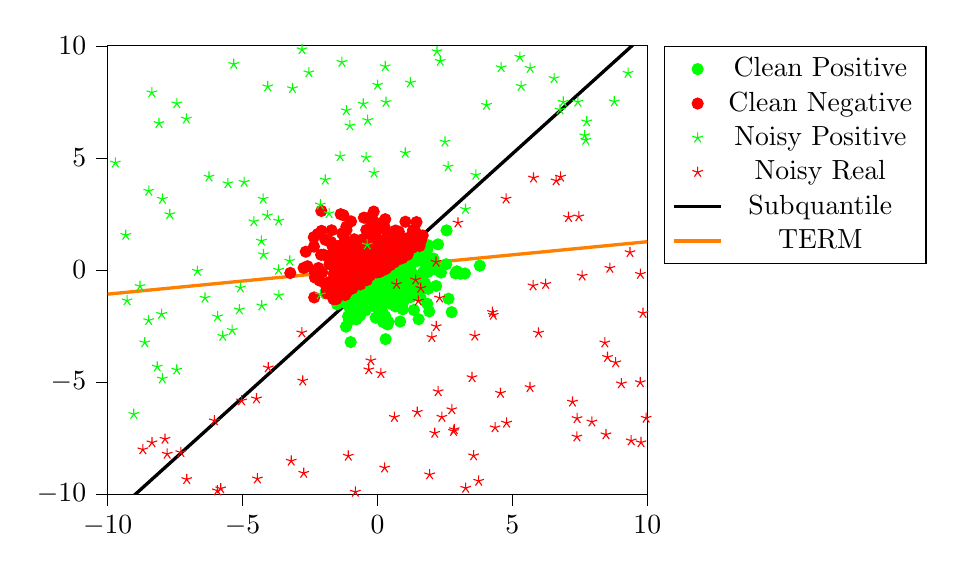
\begin{tikzpicture}
			
			\definecolor{crimson2143940}{RGB}{214,39,40}
			\definecolor{darkgray176}{RGB}{176,176,176}
			\definecolor{darkorange25512714}{RGB}{255,127,14}
			\definecolor{forestgreen4416044}{RGB}{44,160,44}
			\definecolor{steelblue31119180}{RGB}{31,119,180}
			
			\begin{axis}[
				tick align=outside,
				tick pos=left,
				x grid style={darkgray176},
				xmin=-10, xmax=10,
				xtick style={color=black},
				y grid style={darkgray176},
				ymin=-10, ymax=10,
				ytick style={color=black},
				legend pos=outer north east
				]
				\addplot [draw=green, fill=green, mark=*, only marks]
				table{%
					x  y
					0.66615683244066 -1.62717281371022
					0.445952819766562 -1.40613903427429
					1.52394637993167 -2.19777323020149
					2.21456330693041 0.0254188075861247
					0.915499217002861 -0.214796782215287
					-0.197378001137952 -1.12704815750685
					0.436501657732984 -0.160030472278342
					1.23863038232989 -0.0410080721954619
					0.956564533440499 0.27790076592443
					1.22772913484808 -0.817569868767491
					0.731067249104432 -1.0850052746613
					0.489909993591301 -1.50080319469406
					-0.177651984557872 -0.462362335717194
					0.329978440329529 -0.499662195145683
					-0.340493467549488 -0.738272085984057
					-0.742983394051995 -0.859233724094377
					-0.643536982446158 -1.36413902276672
					0.444410931333321 -0.618535187521676
					1.16553309523823 0.0191067283122791
					1.10666258658539 -1.10299839373967
					1.53395046222311 0.644788777043259
					0.963709567518559 0.169517745355712
					0.0331859825344949 -0.36942831866479
					1.8454968669828 -1.50617940688407
					1.81220746174475 0.869792189100366
					0.416736029790476 -0.319638708557343
					0.298016339561939 -1.0709732682338
					2.24333345811497 1.1423558531617
					1.78475499559158 0.58758664746005
					-0.151576968592421 -0.700601923225736
					0.581725811452668 -1.18602167943325
					-0.666231662421854 -1.46512642495228
					0.376200674174538 -0.341959128365558
					0.057287228771993 -0.216839360953207
					0.399314199751391 -2.31257888995466
					0.285518805013539 -2.06436774648733
					0.568919540049707 -0.589892605891152
					0.14185198394922 -0.931846293039823
					-0.32286521786735 -0.480771389668765
					-1.05729107624163 -2.26215456428323
					-0.0764530459803187 -1.65339176066902
					1.27032937617373 -1.12396316195842
					0.797053049152785 0.130029256911551
					0.839096994467804 -2.30116537571806
					0.646292325864762 -0.995381285898413
					0.50871214892843 -0.699382716431272
					2.09240274996592 0.26966550035675
					0.887684862809411 0.335924845827018
					1.00383379222519 -0.139626943174102
					1.14686287136545 0.57781947093845
					-0.0579548308861165 -1.00373210831011
					1.36001649290405 -0.293338779890871
					0.654942917317863 0.226583852596745
					0.377372680129116 -2.42968432401643
					-0.743775722578922 -1.03713686176067
					-1.2983410051037 -1.32303616161292
					0.152572638019352 -0.725290941835232
					1.21410958710833 -0.456676751666631
					0.175627936868847 -0.143870020958486
					1.4755040591781 -1.07079488105621
					0.448812337550431 -0.472597415606296
					0.827494527118024 -0.0297521076026336
					0.571944447729755 0.121335159098297
					1.04555527057162 0.442303141185695
					1.30594793211607 -0.560187072302356
					0.435916169115477 0.130204829120148
					0.813226214722225 -1.07206667451296
					1.70527675591995 -0.198567310702853
					0.624713452957296 -0.863473982991676
					0.888113456108014 -0.807227996774369
					-1.16834797860192 -2.52924937965354
					1.22124935913635 0.430662161826501
					-0.21958420951198 -1.21146483084577
					3.07827557681946 -0.167218174061783
					0.718730143814528 -0.601994811668302
					2.0703809618742 0.511112839122028
					-1.49929254174027 -1.52822867644606
					1.76460806076276 -0.594007894987593
					0.988561120718415 0.00598170883176224
					3.79179189067259 0.192629971405003
					1.01141301412232 -0.150065697539585
					1.15680039832856 -0.0343584601183343
					0.835826245898926 -0.928521363295491
					-0.371902963127745 -0.920113771056722
					1.17520458484326 0.55538933743334
					1.0653026119713 -0.546801552025539
					-0.558968806079548 -0.785223565783628
					1.6734647066364 -0.131659590897679
					-0.00936518211746013 -0.520006678646417
					0.679447039106858 -0.890073276695108
					-0.244365943494025 -0.712781137518178
					1.06254245464988 0.306801793236535
					1.87741149782559 -0.841391614222661
					-0.464205585895658 -0.605211567308329
					-0.585929741894402 -1.53776959439017
					0.0233534207679786 -0.727447919264787
					-0.980181084125299 -1.33345989515339
					2.74762328646669 -1.88170974449462
					0.103257555973976 -0.501961758806969
					0.603374272647579 -0.33046607520118
					-0.52172657100956 -0.664089263536073
					1.39417120680463 0.369473957917061
					1.39503338628941 0.742679979399532
					0.76263381838518 -1.22976553419653
					-0.517147311288648 -1.33130928321311
					0.978387860413117 -0.88252087355011
					0.198108716186294 -0.467181820764147
					1.58583467535759 -1.19222620062697
					-0.267820104818685 -1.3393921286937
					-0.257763662977058 -0.86986567266378
					1.08241483482538 0.314974021837557
					0.114849478169674 -0.25308853014745
					1.0128414272258 -0.92397261524726
					-0.429951222927854 -0.776431785165652
					-1.09134570390344 -2.06927456823446
					1.86474531194525 -0.0928291300283928
					0.235255765088987 -0.641407124575236
					-0.833890755566065 -1.74168304437446
					2.94569146849069 -0.0596058742028795
					0.295944588421379 -0.54612874164333
					-0.944257273666255 -1.13215062031942
					2.18593178649847 0.017773165556573
					0.693859581033236 0.0978957077510147
					0.152517348245513 -0.0856928972155742
					-0.705630634619762 -2.07669381536328
					1.22085817057826 -0.275414123133597
					0.997262686123039 -0.447852309040871
					0.0660179368900788 -0.669665113478782
					-0.145972681493324 -1.05047408642151
					-0.260159659713753 -0.914386700962721
					1.26694873943959 -0.249696817696065
					-0.660092702587763 -1.20049235872884
					0.345007907393673 -0.564287198470257
					0.921289668797954 0.464072538289163
					0.206111880253196 -2.32286369222874
					-1.11745431297186 -1.41010740670945
					0.300386530881327 -3.08781117946191
					1.00851319868084 -0.0909759172870995
					-0.0377381833038066 -0.596755786234033
					-0.253568007807503 -0.387475903061983
					-0.00159165488441168 -0.349848411788577
					-0.647754098519999 -0.92135348982868
					-0.286085357284011 -0.510979833399837
					0.697985032032464 -0.793171657324525
					2.05112091700218 0.307547790467483
					-0.212723145320894 -0.815539913945624
					-0.62342889737268 -1.40251960409244
					-0.785766439133349 -1.22390455652278
					0.192072003440417 -1.13453030140002
					1.03073060814676 0.333774878769359
					1.83327331910728 0.877735295821453
					1.00888069011897 -0.14077746449412
					0.457400472798678 -1.06456392392434
					-0.128771532745256 -1.30268214027347
					0.396594260265474 -0.844633063205176
					0.917985777539228 -0.146261115332306
					0.936018777158661 -1.40542769200449
					0.480902766443747 -0.167952338693885
					0.166573175546728 -1.81698502838628
					0.661810645787002 -0.60527220743406
					1.15102340229127 -1.10788015275747
					0.521846338339786 -1.2221964690405
					0.768376929968135 -0.744109559535043
					-0.994875126801737 -3.21661130195839
					0.184372104833695 -1.19908149509587
					-0.602226806223501 -0.959983790742804
					0.842165500345671 0.0557158077774076
					0.796709307299178 -0.874247321097524
					0.134156676034472 -0.533763925713647
					0.225001195674996 -0.68938635542693
					1.81698031117205 0.0636737860888463
					-0.0177792088307171 -0.463775429917086
					0.592644008223768 -0.960900989290637
					2.63156691241036 -1.28229828101509
					1.11749274441788 -0.187229336098651
					0.475162545487995 -0.275018680119774
					1.38896101496198 -0.939266263896736
					1.36247595498597 0.367210539968479
					0.556110134842152 -0.502701121630064
					-0.276373610167351 -0.978146505685056
					0.0517638758208773 -0.743705837663669
					1.10739919248862 0.100284972810491
					-0.076048041476785 -0.784364865208768
					1.91746486170012 -1.84767545915556
					0.311053469695433 -1.4106736635349
					-0.548980874459089 -1.04363101444589
					1.48065289391744 -0.470086435609679
					0.453530060491717 -1.06320747623897
					0.696754337970094 0.342522763239935
					0.181852220578342 -1.38485286203161
					-0.543793227630678 -0.717262994338622
					0.643916630326197 -1.53593559398699
					1.34500264870188 -0.229159195859251
					0.966039401713727 -1.39619867158147
					0.468139312682519 -0.0595235483505791
					-0.364354695735919 -0.816403853810461
					1.15541720905045 -0.064662281906637
					0.246879871981113 -0.0141422789793296
					0.456239710125811 -0.216659994163216
					2.5447004021849 0.253834154259861
					0.0388024647828259 -0.489777697777351
					0.0979981163830742 -0.197005775951746
					0.348360065202492 -0.673093091237262
					-0.557942507282437 -1.72549489554263
					0.643152751281635 -0.507497472961213
					0.20555450161846 -0.912843469799938
					-1.03418681512832 -1.69450951093734
					-0.303205000532075 -1.01431092570733
					-0.480834640778949 -1.18962563162223
					0.949774008349632 -0.954963274111777
					-0.428113068710892 -0.898493049570657
					0.0646975608836771 -1.09402705301952
					0.133789541512536 -0.138615224916351
					-0.445907842167216 -1.80383360738299
					0.342067288987629 -0.0907274339152934
					-0.7992030595112 -1.87047701186887
					0.808691846551002 -0.397655696205742
					-0.285280858875519 -0.67127811971151
					0.362944603619036 -0.780678125643071
					0.383415077334962 0.056981433574892
					1.31069585721135 0.484039523949239
					-0.839038731165274 -1.33063828459664
					0.92272950370151 -0.653530195504109
					0.494315220341863 -0.522385466398234
					2.17336787685557 -0.713831414521698
					0.708974013723569 -1.0183896814425
					-0.196536984657469 -0.570219067264706
					-0.84354444663676 -1.12332434626361
					0.840830675147263 -1.27893400946671
					1.39278545743231 -0.532161459663105
					1.15865757249051 -0.00967570431742341
					1.87883142509958 1.10395665036258
					-0.0145536260391052 -1.33005402951796
					1.09361648229496 -0.0988991082556169
					-0.153125734176122 -1.26899813589836
					2.55984419020316 1.76643876625804
					1.22255235570963 -1.21349765903271
					1.13528755989253 0.239948023871231
					1.06449445547365 -0.292968037782231
					0.697714586519542 -0.647558900184631
					-0.851296694239478 -1.97699843198895
					1.37301240743036 -0.848913665822315
					-0.629890425834116 -2.00528325086759
					0.278620607720825 -0.324120048412199
					0.252166221033387 -0.959694641000053
					0.120301506361585 -0.454686549528865
					1.61636263669345 0.423302302335542
					0.937585484880203 -1.75397797253351
					-0.580675064064404 -1.53641402217967
					-0.0954846553622515 -0.43128530920453
					0.0119880484134498 -0.238650149117277
					-0.159606621702693 -1.0132143513773
					0.593104831201101 -0.475860166741701
					-0.338953798618382 -0.871315589221875
					1.76109758638034 0.0414973656310206
					-0.47017890212741 -0.749358504112145
					1.30634465737777 0.695272679578708
					0.752909624043016 -1.38622190218933
					0.264829471707753 -0.434479405853107
					0.462585642051635 -0.814152802226493
					0.408892359548374 -0.250838343507271
					2.88747056441761 -0.151677469875436
					-0.214476206645097 -0.456568172687176
					0.891323410580167 -0.714048258644193
					-1.14476991098454 -1.49993688940828
					0.513378660080797 0.179335337309763
					0.437494600955555 0.0804651426135801
					-0.782426397511638 -2.20181103833646
					0.0117857243919593 -0.695916177019542
					0.365703496202358 -0.670011604275127
					-0.702770824286091 -1.32125157160233
					0.222057518072767 -1.14566468281996
					1.34709802470378 -1.78501255435017
					0.997634143539367 -1.27901457508704
					0.366690271026193 -0.431808559134697
					0.709936640808344 -0.247206953699368
					0.453688012804473 0.0726616700392308
					0.548594157645974 0.0136598146485003
					2.35293962099882 -0.11616086671906
					0.692079962024725 -0.215228894627227
					1.56886603669161 -0.576016007602282
					3.24130472176104 -0.157318423520625
					-0.0668627701841508 -2.13256955145518
				};
				\addplot [draw=red, fill=red, mark=*, only marks]
				table{%
					x  y
					0.475236336848592 0.463012444226059
					0.967699379163849 0.92140572272952
					-0.668224444347855 0.0134100776815537
					-1.59801652038155 0.801902526105908
					-0.652240344749113 -0.0876446835888625
					-0.776235087388337 0.143433587631849
					-0.144910289729945 0.556381332037456
					-1.43433917928222 1.06767671364788
					-2.14298903496561 -0.47360076620765
					0.790454964600858 1.70967210176251
					0.123862930193482 -0.0343663915529025
					-0.815598485812531 -0.370435046289001
					-0.487817657729491 1.11001964252755
					-0.2977411911839 1.00712351678466
					-0.70842489040164 -0.378326958596883
					0.179947172657584 2.1162921203765
					-1.16518836608074 -0.103325729993843
					-1.61859036754761 -0.184094647376469
					-0.377878836844027 2.30680294360327
					-1.53820010110939 -0.845521935287509
					-0.0333994465221774 0.368814301116742
					-1.08503107943463 0.112988612998402
					0.430383060962107 0.210923121187864
					0.468169051085977 0.88003338933485
					0.942097700700458 0.737517397346816
					-0.961328794031092 0.946408317154522
					0.42783531184974 0.214017643340661
					-0.739853558879982 -0.540530555065235
					0.546805397941593 0.965154662763188
					-1.44694404606385 -0.191638248668145
					-1.50809034396094 -0.563942672514444
					-0.226221441068309 -0.0833812653410768
					-1.04295264671769 -0.0262556864066846
					-0.789376628404095 0.0260116033209758
					-0.409522950216095 -0.099403119417888
					-1.53708490105798 -0.48708185506254
					0.351074085073525 1.04028659372602
					-0.377537462223265 0.166478453927596
					0.0696114274143889 0.0771371982977744
					-1.8247252340206 0.619409907068839
					-0.504998831807743 2.33266227135881
					-0.64406537575134 0.199128884904459
					-0.192324497392816 2.15929823627506
					-1.78067810484484 0.250418659849534
					0.347820976604145 1.24578209082999
					-0.463432337950987 0.257756798298679
					0.950426270167282 1.20223564922803
					-1.50610050504903 0.0469478789542146
					-0.366771806425449 1.40939573803927
					-0.855617357329685 0.924985665416845
					-0.498643021165629 1.02184362125819
					-1.52193033054128 0.890247054910075
					-0.257463561592124 -0.110229620787321
					-0.434188549565844 -0.193424559283797
					0.589974282966134 1.51796954198617
					-0.638324126389838 -0.454171309289274
					-0.774532370088533 -0.515218407622761
					-2.31948385212898 -0.336798017646946
					-1.28854481722462 0.837532494659673
					-0.465470431704765 0.61294291847272
					0.58537534617129 0.971266099856424
					-0.258455090120113 0.227830808925707
					1.54932197250706 1.4807785917022
					-0.139082885742803 1.13591056282581
					0.423114661282241 0.379404128965843
					-1.30960608638426 1.6329553105073
					-0.893616361865074 -0.376819305136002
					-0.32845374075451 1.25641123595498
					-0.649204713086565 0.991494555058154
					-0.540021559663908 0.212287840257359
					0.84350821461945 0.637275155042302
					-0.205753602946921 1.04559961536316
					-0.922066952270587 -0.801547878096031
					-0.769936308110319 0.0117168553241757
					0.131868499164814 -0.0154912771117235
					-0.123549800562307 1.0744069070268
					-0.843616199762684 0.423615871745404
					-0.26834464941644 1.14521059324374
					0.0415601024400449 0.0341765179693585
					1.3658086705989 1.12307827669423
					0.895365557931236 0.630917133531121
					1.28608206333689 0.984166860859365
					-0.735082921797092 1.03066071172153
					-0.797767897793636 1.26427327753595
					-2.59259632664383 0.165569998870663
					-0.693038456041847 0.152421896352347
					-0.860516448307554 1.36897786176098
					0.941594308193752 0.772563176374906
					-0.388185725437337 1.30180371318981
					-0.696952705821732 -0.408264485170377
					-2.31906192927273 -0.115776571361874
					-0.568987692185994 1.2243010032147
					-1.6955056829236 1.1442959755204
					-0.851940963952884 -0.323177501266217
					-1.43207419229316 0.437128776146755
					0.364085742847483 1.64969530511649
					-2.34676299310436 -1.22582618082679
					0.265755177615246 1.90237232653499
					0.890559238598946 0.947972236309174
					-1.99674786351352 0.68224737950016
					1.09037734557583 0.666957453654226
					-0.497455748375109 0.586649011800615
					0.248154658023625 1.11688590979617
					-1.03714928844058 0.487581498419587
					-0.684987212746847 -0.047232567452791
					-0.247374194967595 -0.0384225078411706
					0.689073496368205 0.937461118474827
					-1.35008121576029 -0.815577710790118
					0.17605554686618 0.305565390663524
					-2.36009374991355 1.46300309967372
					1.31188545180201 1.76695327351986
					1.07919058288908 1.10813670512442
					-0.592707599683219 0.848574081875953
					-0.510055672444058 -0.333825650769236
					1.06197315615708 1.25556508092997
					-2.08181334267585 2.63322359919665
					-0.373619699036781 0.97546828746837
					0.0331167302276345 -0.0552687932595129
					-0.140566678977075 2.60427720950297
					-0.149938869498326 1.01572775726338
					-0.191262029375551 0.539233052049219
					-0.454393716193247 0.613660985492747
					1.49915059316412 1.51918164092086
					0.323394654245515 0.668356261277103
					-2.05148718253001 -0.105748010770523
					-0.189670732050936 1.54350214466163
					-1.91555771638286 -1.03645673483894
					-0.758258863686268 -0.56465164324571
					1.08775969474541 1.34186883584486
					0.38247361840119 0.252547221568943
					0.475257058261301 0.713326251943562
					-0.652819687938335 0.303465371691839
					1.06935316307576 0.866233770674405
					0.114778959190959 0.77311570178277
					-0.817934045024551 -0.00967732608339573
					-1.18011284291271 -0.429908171089784
					-0.619201714146259 -0.207776034082217
					-0.21948303968429 0.399402124502037
					0.14260066994415 0.409564065690522
					1.36228935352407 1.44151146733257
					-0.0466723369267926 0.601202650478886
					0.642263162434125 1.20056202222963
					-0.854222795081366 0.384233963841323
					-2.07409331483507 1.7444016769278
					-0.278983724612909 0.337692508883196
					-1.19668092284026 -1.11878538046637
					-1.91059837823497 -0.664507035850071
					-1.0504535717056 -0.254309316642444
					0.0334743611472721 1.34587998341365
					-1.27148724860631 0.74526884125347
					-1.48797222173224 1.0019742616917
					-1.38685851850937 0.274951757326178
					-0.948986123159582 1.10764813982932
					-0.654835193813054 0.0165134911117578
					-0.227746370289367 0.319161079518604
					-0.488876757801558 -0.272449963331595
					0.018455064746596 1.79694807790083
					-0.623981680368234 -0.40742620107593
					0.287218716414353 2.26519396756006
					0.241291968999512 0.365512794063371
					-0.305689971347232 0.241569369333787
					-1.55372879710895 -0.566297743714184
					1.25766125144705 1.26978450590392
					0.399242697242191 0.931929065730117
					-0.579394020791606 0.649441957191073
					-1.20034442529592 0.732113507974711
					1.60943489632249 1.30297584636534
					-1.21022163243129 -0.516434958768904
					-0.436212967398389 -0.0372964441019841
					0.731804570325532 1.50117478968416
					-0.54532007611853 0.0987258847903623
					-0.372724546313458 -0.118495727340943
					-0.977856047511215 0.238188179210828
					0.0587266696030722 0.979724768049228
					0.0279651690579889 1.00932142902679
					-0.554952502560571 0.00394861105604572
					0.60702156916613 0.620755317317189
					-1.22469750790432 1.25542357582705
					-1.49582980600297 -0.365111390871
					-0.352505434769658 -0.137299941657116
					-0.992066919154765 -0.245334131479329
					-0.4541458614843 0.362789609089358
					-1.14436928816638 0.426141485511969
					1.44541432219832 2.13630548791369
					-1.28284925101596 -0.511521761908962
					-0.0578486487707841 0.689319179262006
					0.269573767506197 0.245500451587538
					0.266510843659414 0.0244370673887122
					-1.02760063629754 0.353577959081655
					-0.33874934627099 1.0779762642348
					-1.20326224475745 1.27925489755267
					-1.05823232979556 1.02391181338029
					-0.959321030785654 0.699300536760086
					-0.749561053847946 -0.221310143236409
					-1.18231133062371 0.779836619873515
					-0.637352705341048 -0.644452984082947
					-0.668509812975555 0.276176078793475
					-1.2141517996553 0.480535693861733
					-0.150297692179263 0.510453439630174
					0.10356673475735 0.953800187301366
					-0.052436597804839 -0.0459711978572278
					-0.949240315769266 0.814658038405427
					0.154004158508115 0.0378979412123706
					-0.450239993487605 0.932626594892052
					-0.428948250806265 1.08244281205456
					-0.955279982868013 0.827243152584127
					-2.19142804671317 0.0863280448006954
					0.376080786455449 0.40830874846197
					1.22815708202172 1.05134208134211
					-1.14126934760024 -0.986714378233963
					-0.137884439615041 0.0804940044917133
					0.35874485120062 0.90751582091846
					-1.0461259330452 -0.130182403227734
					-2.65844996844804 0.814207199654882
					0.300922575960277 0.5279317768804
					-0.372168508419197 1.04639129852736
					0.363058009811838 0.36655849572181
					-0.431131822338247 0.293960646621104
					-1.64390709807731 1.00379369397516
					0.289679019511758 0.875227339677769
					1.11869301811118 0.697971862502518
					-0.0604648858650206 1.10562737391484
					-0.0911496360596119 1.2909980247463
					-0.532785735025644 -0.387701523024233
					0.606817839881207 0.332177918899453
					0.202057411410521 0.0105480551463527
					-1.65683264672341 -1.19263103232517
					-0.304900480360123 0.733703196035257
					0.409382432691112 0.590214128788059
					0.386641165084585 1.01295793867112
					0.505601047686351 0.489390493922675
					-0.477601917301834 -0.147905373227185
					-1.31322541294477 -1.08840645439629
					-0.985234277041191 1.16349842661756
					0.0876427628767861 0.543797780058774
					-1.54304772768096 -0.313511783732468
					-1.73910651865567 -0.686561525374017
					0.545542341533929 1.3098128495424
					-1.30636859516473 0.389673445897781
					-0.216031013420479 0.550417047462993
					-0.0836627165144513 0.168002993330269
					-1.25873698019103 1.5673801976152
					-1.1514159340436 1.77662532917969
					1.37746294452066 1.78795882021144
					0.176370480457864 0.133320679662724
					-1.14865572954751 0.490788563020659
					-1.12099272621409 -0.201625194856154
					-3.23176223668939 -0.135607347832726
					0.146531671691386 0.297214508094128
					0.90223476027313 1.21229880809425
					-0.440923325239559 0.143732148543258
					-0.7523603147915 1.11089250550745
					-0.477748087437791 -0.0463553873706611
					-1.59670990785929 0.677960632961314
					-0.569908008642468 1.17460961098909
					1.11151464592744 1.03099717734552
					0.702199598961228 0.681181261309853
					0.68737016385428 1.48351494905725
					-0.524996909257634 1.01474133390266
					-1.35691288892772 0.93690544370851
					1.14157509593154 1.43230005311393
					-1.63489951231451 -1.2946848959764
					1.14538767028128 1.14198550685694
					-0.534867252649906 0.422578311341804
					0.137137751605839 0.224243699218158
					-0.149821792602388 0.501085239496564
					-2.21663733619343 1.5996502144226
					-0.478491575769657 0.386774024963858
					-1.51257657992101 1.05712922446285
					-0.0572633616384909 -0.0805204177487055
					0.0821223873385324 0.953258959844344
					1.38245884958011 1.57774611143816
					0.501025721994447 0.397002772054341
					-1.78988032509101 0.51651085800864
					-1.0548228212559 -0.545288447602914
					-0.0497892662483036 1.75853764273025
					0.0950321141314446 0.643144188302977
					0.758465677321738 0.460065123008359
					-0.529292695425762 0.222822958950593
					-0.401474600747842 -0.280602951207461
					0.0293373249127382 0.826582007280199
					0.339696604859773 0.624804682780002
					-1.93175278578442 1.34680074155415
					-2.73821796341825 0.0869278764543989
					-0.417851975799902 -0.405434009833702
					-0.41727686360872 0.445281563787134
					0.460352681763873 1.27267138990024
					-0.287057112083017 0.0217304990211649
					-2.09152164736398 0.676922288000271
					-1.52587765204009 -1.29818460723047
					-2.27166137222418 -0.0959556787202743
					-0.280875933867878 -0.248614625211493
					-0.687574162901349 0.068628906905953
					-1.55714604429926 -0.118691277537513
					-1.36403480378502 2.48867589178021
					0.0412837136000159 0.133899237091134
					-1.90542173959687 -0.70668655819936
					-0.629179879462959 -0.37499492727148
					0.106217409222432 1.91669961771955
					-0.141890281995137 0.215519869406797
					-0.125510068126207 0.110984525023682
					1.03483925489568 2.15117592369137
					-1.78420522994159 -0.598467708048519
					-1.25953312500264 2.43932114175752
					0.294213772100445 0.343988071536462
					-0.556647273811506 1.36604875025868
					-0.897162843995725 0.776241049002083
					-0.250079230915721 1.17096408969735
					0.485673568562834 1.13388228518267
					1.67439988788449 1.5390002735853
					-2.35528632467087 1.04139476391334
					0.285314566229577 0.262345313810231
					0.474316236501489 0.216520628496499
					-1.81295659791369 -0.551311136865345
					-1.43615199739193 0.16270429301717
					0.668232102465844 1.7587156978153
					-1.18923399951177 -0.511860477017393
					-1.42784073059871 -0.0244536724747458
					-0.467733253144623 -0.162187631945196
					-0.887436401611487 0.104705329500114
					-1.72331845220832 1.24768152947971
					-0.846876088797259 -0.116544408199708
					0.727177546488967 0.639031172020778
					-0.906877551793352 0.112284686310808
					-0.167056051111615 2.21219513969865
					-0.0375278989026581 -0.107956535107795
					0.0607569824748015 0.0321670436669549
					-0.947864900582108 -0.832405899389923
					-0.941449095208048 0.814987989077706
					-1.12185021985355 -0.192294314501207
					-1.15423383167972 1.93005674044744
					0.997386961501991 1.39734885274957
					-1.11499188858092 0.111473284852295
					0.225727780929115 0.919243201650782
					-0.347080203921073 1.33188463197374
					-1.70191702905596 1.76958989738775
					-0.0238075446494345 0.0207632012919808
					-0.281715664073061 0.257744626195243
					-0.239318167358479 0.651260367495504
					0.746294143171406 1.03864055005515
					-1.44199729575478 -1.02944419418072
					0.0654262628963858 -0.0929007076304017
					-0.98141008437662 2.16845376525774
					-0.688833669137282 -0.396196518810751
					0.327486360463712 0.0833469643741777
					-0.208371516679103 0.560718803116551
					-0.437615916055019 1.11983245073609
					-1.49324493303948 -0.0964609550843266
					-1.18645863758121 0.301399869461525
					-0.89094515683642 -0.0511190243288162
					-1.01227144693191 0.132793049611791
					-0.415909700706841 1.78494368334
					1.56007836658786 1.06954656601913
					0.919189867052444 0.529393066514192
					-0.234816588383113 1.33883664213584
					-0.398790418391939 -0.450931206119549
					-0.458086211781045 0.974583193470235
				};
				\addplot [draw=green, fill=green, mark=star, only marks]
				table{%
					x  y
					0.00521654927563731 8.24838170244221
					-0.364325449231938 6.67839061123626
					-4.94381373163028 3.91877756201801
					0.286859727262595 9.07747258653718
					-7.699980046388 2.47797069893767
					-5.11897074947789 -1.76819896797575
					7.67873953514165 5.99939334075555
					6.88418230219515 7.49291933198486
					-0.420142612842735 5.01535057075621
					-1.79514636426437 2.52337425597134
					-4.22589266363797 0.691218699414369
					-0.1277059333861 4.33232362328009
					-3.6680111277136 -0.00148499820439518
					-4.58327247778936 2.16148391504915
					-5.54415862199862 3.85769818402351
					3.26017818297636 2.7128496997773
					-6.39315547118538 -1.24870101445722
					-9.03284947007994 -6.43332535134111
					-3.25309552087984 0.400852354369158
					-4.08214049627146 2.42352859877473
					2.20348258688806 9.75017298417442
					-7.44201821632009 -4.45720138346793
					6.54556136408697 8.54703447369846
					8.77501725185272 7.50889238613447
					-3.15119556202299 8.09933040482508
					-8.62557010373087 -3.24186128381512
					-4.30246902415033 1.29610361720319
					-2.79874380354891 9.83464707341237
					-7.08378291902247 6.73900553715143
					-2.11868999242737 -1.09791010007726
					-6.24530657796112 4.15537325716365
					-0.382572697107353 1.12415363975535
					-8.48172914079312 -2.25007735006485
					-3.66410701069501 2.19101699050787
					-4.06788889893845 8.18021261790674
					-4.28914603985302 -1.59449578230125
					-3.6553318912254 -1.13553947344245
					-1.38514460606613 5.06296624659696
					4.58349501377899 9.03504911038683
					-1.93472894933817 4.0213221976016
					-1.15534972140304 7.11092667481105
					-6.67375592975234 -0.0481576816568623
					-2.5442952320304 8.8058374976326
					2.61747747848061 4.60433838835615
					-2.11946928943648 2.9105542626305
					-8.80212615239411 -0.725885220902578
					0.315893110959269 7.48347796267154
					-5.08139510825616 -0.796289208795711
					-7.97444576408826 -4.85267571901176
					4.0411995600374 7.35487128060059
					1.02855977124216 5.21938166753445
					-5.32873960930913 9.1817743428695
					7.75354126947769 6.61526335296249
					-4.23834121691478 3.16572184238932
					-9.71622176853268 4.78089243766008
					-7.97123675668076 3.16496401666998
					-8.09977012675128 6.54270583095456
					-5.7363151722882 -2.95325773507678
					-1.31883316442224 9.27025593043499
					-9.28169509228633 -1.36621143381482
					-1.02343812844493 6.43725367749741
					-5.38781986633503 -2.68578993520594
					2.32507956530892 9.31584268859279
					5.32271153991234 8.20160388701892
					2.50160793620673 5.71697127550053
					5.27621038652075 9.4976716924894
					-8.00328538373134 -1.96999174230703
					-8.16326131318811 -4.32133038772382
					7.71755754740555 5.79303286405154
					-0.529550055761252 7.40654340444653
					3.64545523165352 4.23604986110871
					7.42434717911502 7.49776807114322
					1.22008038724765 8.35263353776215
					5.6581320601877 9.0026287137526
					-8.36300990166375 7.91433427747252
					9.28614801257253 8.78054843386492
					-5.92769659673442 -2.08396061532142
					-8.47596982843674 3.52193517290124
					-9.32942873393278 1.55327586000583
					-7.43562019993761 7.42537331485811
					6.76167970610025 7.14563099123019
				};
				\addplot [draw=red, fill=red, mark=star, only marks]
				table{%
					x  y
					9.03889835069221 -5.070588209875
					-4.04957209646065 -4.35832546951773
					-8.69748468173608 -8.01275562063259
					2.84428686470481 -7.11490705954094
					4.55781529951811 -5.49358411431467
					2.30006591126446 -1.24271013238955
					6.232411753148 -0.635411486394338
					7.39093184915033 -7.44185107662353
					1.47494911824863 -6.343430283491
					-7.79474442665031 -8.20893391444845
					-3.19844048353151 -8.52010020444683
					5.96750736114124 -2.80417094632465
					-5.81105816748038 -9.75208791577634
					7.07865201159824 2.35063956319274
					4.29057823134713 -2.01173349514965
					-7.06984640910915 -9.34078940055675
					7.46162547527741 2.38062065354794
					4.78368321117814 -6.82380246479634
					4.76572731802522 3.17272963476243
					2.17831016518105 -2.51935464341219
					-7.28985528381079 -8.13959163130178
					7.22551199449262 -5.88390376944583
					9.83943550354005 -1.92765086326555
					-7.87527181606039 -7.54312727395711
					7.39650286649022 -6.62005609387501
					-1.08274873748598 -8.29821073342332
					2.75444410142905 -6.22522493666154
					2.81690969679751 -7.19307336865911
					8.82737296287756 -4.13109937804854
					-8.35916247712585 -7.70188777321223
					-2.77181527372403 -4.94513891693759
					1.5124019121642 -1.38132248222691
					8.42441963324625 -3.24569951623054
					6.78422975531402 4.15043879319779
					9.73895486670127 -5.01731238186648
					1.93165481890317 -9.1295439130818
					5.78332769535998 4.10958768433427
					-5.93446176075567 -9.84486509457596
					-0.820735514703879 -9.9049159677701
					3.26732700846112 -9.72903931077728
					9.35859426059814 0.78247712431728
					-5.03686156102109 -5.83138783989801
					-0.322577369553898 -4.44557130956193
					0.626907084086357 -6.56802644269894
					8.61050664468787 0.0844973504513735
					3.56084987907079 -8.28327387416041
					0.127108161582491 -4.61147100918152
					-4.45109749577109 -9.31386075477692
					2.38536614411984 -6.56182352512698
					3.60760730569839 -2.94030178049522
					1.60457170812276 -0.810121725384105
					-2.80539617410531 -2.79646789677662
					2.2470426794088 -5.41920782987576
					2.98261846193727 2.10497333200417
					-6.04508118530369 -6.72315165195995
					9.40209876002844 -7.61523859562385
					2.01346074925556 -3.00234451022094
					8.52522381525819 -3.89151475218842
					4.2589445686631 -1.8867198768605
					6.62049483166934 3.98269024084068
					5.65260337420258 -5.23708718832513
					0.706632004809356 -0.63781865419605
					9.95640294431649 -6.60540536036044
					-0.246634935406945 -4.04036939082358
					7.94623070937174 -6.77318177297525
					-2.73485510989851 -9.06085687410654
					2.12158077255907 -7.27656725150748
					5.76487453761642 -0.701616489516933
					-4.4853675106036 -5.74128139957419
					9.74327515780177 -0.186048277424128
					8.46704934141416 -7.34319059105631
					7.58456023196645 -0.26272801085166
					1.41178738483809 -0.439188887421079
					2.16952440028389 0.355129475328294
					9.76690514271873 -7.69743187522739
					4.3570525890475 -7.0300672484968
					0.265320455433915 -8.82533590954626
					3.50390097688804 -4.7941718914602
					3.74978281954121 -9.41547013235786
				};
				\addplot [very thick, black]
				table {%
					-10 -11.1217698790111
					-9.7979797979798 -10.9021671187125
					-9.5959595959596 -10.6825643584139
					-9.39393939393939 -10.4629615981153
					-9.19191919191919 -10.2433588378167
					-8.98989898989899 -10.0237560775182
					-8.78787878787879 -9.80415331721959
					-8.58585858585859 -9.58455055692101
					-8.38383838383838 -9.36494779662243
					-8.18181818181818 -9.14534503632384
					-7.97979797979798 -8.92574227602526
					-7.77777777777778 -8.70613951572668
					-7.57575757575758 -8.48653675542811
					-7.37373737373737 -8.26693399512952
					-7.17171717171717 -8.04733123483094
					-6.96969696969697 -7.82772847453236
					-6.76767676767677 -7.60812571423378
					-6.56565656565657 -7.3885229539352
					-6.36363636363636 -7.16892019363662
					-6.16161616161616 -6.94931743333804
					-5.95959595959596 -6.72971467303946
					-5.75757575757576 -6.51011191274088
					-5.55555555555556 -6.2905091524423
					-5.35353535353535 -6.07090639214372
					-5.15151515151515 -5.85130363184514
					-4.94949494949495 -5.63170087154656
					-4.74747474747475 -5.41209811124798
					-4.54545454545455 -5.1924953509494
					-4.34343434343434 -4.97289259065082
					-4.14141414141414 -4.75328983035224
					-3.93939393939394 -4.53368707005366
					-3.73737373737374 -4.31408430975508
					-3.53535353535354 -4.0944815494565
					-3.33333333333333 -3.87487878915792
					-3.13131313131313 -3.65527602885934
					-2.92929292929293 -3.43567326856076
					-2.72727272727273 -3.21607050826218
					-2.52525252525253 -2.9964677479636
					-2.32323232323232 -2.77686498766502
					-2.12121212121212 -2.55726222736644
					-1.91919191919192 -2.33765946706785
					-1.71717171717172 -2.11805670676928
					-1.51515151515152 -1.89845394647069
					-1.31313131313131 -1.67885118617211
					-1.11111111111111 -1.45924842587353
					-0.90909090909091 -1.23964566557495
					-0.707070707070708 -1.02004290527637
					-0.505050505050505 -0.800440144977792
					-0.303030303030303 -0.580837384679212
					-0.1010101010101 -0.361234624380631
					0.1010101010101 -0.141631864082052
					0.303030303030303 0.0779708962165289
					0.505050505050505 0.29757365651511
					0.707070707070708 0.517176416813691
					0.909090909090908 0.736779177112269
					1.11111111111111 0.95638193741085
					1.31313131313131 1.17598469770943
					1.51515151515152 1.39558745800801
					1.71717171717172 1.61519021830659
					1.91919191919192 1.83479297860517
					2.12121212121212 2.05439573890375
					2.32323232323232 2.27399849920233
					2.52525252525252 2.49360125950091
					2.72727272727273 2.71320401979949
					2.92929292929293 2.93280678009807
					3.13131313131313 3.15240954039665
					3.33333333333333 3.37201230069523
					3.53535353535353 3.59161506099381
					3.73737373737374 3.81121782129239
					3.93939393939394 4.03082058159098
					4.14141414141414 4.25042334188956
					4.34343434343434 4.47002610218814
					4.54545454545454 4.68962886248672
					4.74747474747475 4.9092316227853
					4.94949494949495 5.12883438308388
					5.15151515151515 5.34843714338246
					5.35353535353535 5.56803990368104
					5.55555555555556 5.78764266397962
					5.75757575757576 6.0072454242782
					5.95959595959596 6.22684818457678
					6.16161616161616 6.44645094487536
					6.36363636363636 6.66605370517394
					6.56565656565656 6.88565646547252
					6.76767676767677 7.1052592257711
					6.96969696969697 7.32486198606968
					7.17171717171717 7.54446474636826
					7.37373737373737 7.76406750666684
					7.57575757575757 7.98367026696542
					7.77777777777778 8.203273027264
					7.97979797979798 8.42287578756258
					8.18181818181818 8.64247854786116
					8.38383838383838 8.86208130815974
					8.58585858585858 9.08168406845832
					8.78787878787879 9.30128682875691
					8.98989898989899 9.52088958905548
					9.19191919191919 9.74049234935406
					9.39393939393939 9.96009510965265
					9.5959595959596 10.1796978699512
					9.7979797979798 10.3993006302498
					10 10.6189033905484
				};
				\addplot [very thick, orange]
				table {%
					-10 -1.0776316909655
					-9.7979797979798 -1.0540171095457
					-9.5959595959596 -1.0304025281259
					-9.39393939393939 -1.0067879467061
					-9.19191919191919 -0.983173365286306
					-8.98989898989899 -0.959558783866506
					-8.78787878787879 -0.935944202446707
					-8.58585858585859 -0.912329621026908
					-8.38383838383838 -0.888715039607109
					-8.18181818181818 -0.86510045818731
					-7.97979797979798 -0.841485876767511
					-7.77777777777778 -0.817871295347712
					-7.57575757575758 -0.794256713927913
					-7.37373737373737 -0.770642132508113
					-7.17171717171717 -0.747027551088314
					-6.96969696969697 -0.723412969668515
					-6.76767676767677 -0.699798388248716
					-6.56565656565657 -0.676183806828917
					-6.36363636363636 -0.652569225409118
					-6.16161616161616 -0.628954643989319
					-5.95959595959596 -0.60534006256952
					-5.75757575757576 -0.58172548114972
					-5.55555555555556 -0.558110899729921
					-5.35353535353535 -0.534496318310122
					-5.15151515151515 -0.510881736890323
					-4.94949494949495 -0.487267155470524
					-4.74747474747475 -0.463652574050725
					-4.54545454545455 -0.440037992630926
					-4.34343434343434 -0.416423411211127
					-4.14141414141414 -0.392808829791327
					-3.93939393939394 -0.369194248371528
					-3.73737373737374 -0.345579666951729
					-3.53535353535354 -0.32196508553193
					-3.33333333333333 -0.298350504112131
					-3.13131313131313 -0.274735922692332
					-2.92929292929293 -0.251121341272533
					-2.72727272727273 -0.227506759852734
					-2.52525252525253 -0.203892178432934
					-2.32323232323232 -0.180277597013135
					-2.12121212121212 -0.156663015593336
					-1.91919191919192 -0.133048434173537
					-1.71717171717172 -0.109433852753738
					-1.51515151515152 -0.0858192713339388
					-1.31313131313131 -0.0622046899141397
					-1.11111111111111 -0.0385901084943405
					-0.90909090909091 -0.0149755270745415
					-0.707070707070708 0.00863905434525765
					-0.505050505050505 0.0322536357650568
					-0.303030303030303 0.055868217184856
					-0.1010101010101 0.0794827986046552
					0.1010101010101 0.103097380024454
					0.303030303030303 0.126711961444253
					0.505050505050505 0.150326542864053
					0.707070707070708 0.173941124283852
					0.909090909090908 0.197555705703651
					1.11111111111111 0.22117028712345
					1.31313131313131 0.244784868543249
					1.51515151515152 0.268399449963048
					1.71717171717172 0.292014031382847
					1.91919191919192 0.315628612802646
					2.12121212121212 0.339243194222445
					2.32323232323232 0.362857775642245
					2.52525252525252 0.386472357062044
					2.72727272727273 0.410086938481843
					2.92929292929293 0.433701519901642
					3.13131313131313 0.457316101321441
					3.33333333333333 0.48093068274124
					3.53535353535353 0.504545264161039
					3.73737373737374 0.528159845580838
					3.93939393939394 0.551774427000638
					4.14141414141414 0.575389008420437
					4.34343434343434 0.599003589840236
					4.54545454545454 0.622618171260035
					4.74747474747475 0.646232752679834
					4.94949494949495 0.669847334099633
					5.15151515151515 0.693461915519432
					5.35353535353535 0.717076496939231
					5.55555555555556 0.740691078359031
					5.75757575757576 0.76430565977883
					5.95959595959596 0.787920241198629
					6.16161616161616 0.811534822618428
					6.36363636363636 0.835149404038227
					6.56565656565656 0.858763985458026
					6.76767676767677 0.882378566877825
					6.96969696969697 0.905993148297624
					7.17171717171717 0.929607729717424
					7.37373737373737 0.953222311137223
					7.57575757575757 0.976836892557022
					7.77777777777778 1.00045147397682
					7.97979797979798 1.02406605539662
					8.18181818181818 1.04768063681642
					8.38383838383838 1.07129521823622
					8.58585858585858 1.09490979965602
					8.78787878787879 1.11852438107582
					8.98989898989899 1.14213896249562
					9.19191919191919 1.16575354391541
					9.39393939393939 1.18936812533521
					9.5959595959596 1.21298270675501
					9.7979797979798 1.23659728817481
					10 1.26021186959461
				};
				\legend{Clean Positive, Clean Negative, Noisy Positive, Noisy Real, Subquantile, TERM}
			\end{axis}
			
		\end{tikzpicture}
		\caption{Logistic Regression}
	\end{figure}
	We will describe the inliers and outliers:\\
	Inliers: $x_{\operatorname*{in}} \sim \mathcal{N}(0,I_2)$, $\vw \sim \mathcal{N}(0,I_2)$, $b \sim \mathcal{N}(0,1)$, $y|\vx \sim \operatorname*{sign}\left(\mathcal{N}(\vx\vw +b, 0.01)\right)$\\
	Outliers: $x_{\operatorname*{out}} \sim \mathcal{U}\left(\left[-10,10\right]^2\right)$, $y|\vx \sim \operatorname*{sign}\left(-\vx\vw -b\right)$\\
	$x_{\operatorname*{train}} = 800$, $X_{\operatorname*{test}} = 200$\\
	
	Our comparisons are only against other robust meta algorithms.
		\begin{table}[!h]
		\centering
		\begin{tabular}{lcccc}
			\toprule 
			\textbf{Objectives}&\multicolumn{4}{c}{Test RMSE (\texttt{Logistic Regression})}\\                   
			\cmidrule(rl){2-5}
			&\subhead{$\eps = 0.1$}& \subhead{$\eps = 0.2$}& \subhead{$\eps = 0.3$} & \subhead{$\eps = 0.4$}\\ 
			\midrule
			ERM  &$0.620_{(0.0200)}$&$0.523_{(0.0299)}$ & $0.648_{(0.2958)}$ & $0.660_{(0.2817)}$\\
			TERM \cite{li2020tilted} &$0.640_{(0.0067)}$&$0.642_{(0.0088)}$ & $0.549_{(0.0263)}$ & $0.041_{(0.0267)}$\\
			SEVER \cite{DiakonikolasKKLSS19} &$0.786_{(0.1357)}$&$\mathbf{0.810_{(0.1290)}}$ & $0.767_{(0.0717)}$ & $\mathbf{0.872_{(0.0731)}}$\\
			\rowcolor{LightCyan}
			SubQuantile &$\mathbf{0.950_{(0.0500)}}$&$0.707_{(0.1825)}$&$\mathbf{0.802_{(0.1619)}}$ & $\mathbf{0.875_{(0.1355)}}$ \\
			\midrule 
			Genie ERM &$1.000_{(0.000)}$&$1.000_{(0.000)}$ & $1.000_{(0.000)}$& $1.000_{(0.000)}$\\
			\bottomrule
		\end{tabular}
		\caption{\texttt{Logistic Regression}. Test accuracy on $P$. Subquantile is trained with $p = (1 - \eps)$ and max $32$ iterations.}
		\label{tab:logistic-regression}
	\end{table}

	\subsection{Support Vector Machine (SVM)}
	The objective function for SVM is:
	\begin{equation}
		f(\vtheta) = \frac{1}{n} \sum_{i=1}^n \left(1 - y_i \left(\vtheta \mX_i\right)\right)_+
	\end{equation}
	We will describe the inliers and outliers:\\
	Inliers: $x_{\operatorname*{in}} \sim \mathcal{N}(0,I_2)$, $\vw \sim \mathcal{N}(0,I_2)$, $b \sim \mathcal{N}(0,1)$, $y|\vx \sim \operatorname*{sign}\left(\mathcal{N}(\vx\vw +b, 0.01)\right)$\\
	Outliers: $x_{\operatorname*{out}} \sim \mathcal{U}\left(\left[-10,10\right]^2\right)$, $y|\vx \sim \operatorname*{sign}\left(-\vx\vw -b\right)$\\
	$x_{\operatorname*{train}} = 800$, $X_{\operatorname*{test}} = 200$\\
	
	Our comparisons are only against other robust meta algorithms.
	\begin{table}[!h]
		\centering
		\begin{tabular}{lcccc}
			\toprule 
			\textbf{Objectives}&\multicolumn{4}{c}{Test RMSE (\texttt{Support Vector Machine})}\\                   
			\cmidrule(rl){2-5}
			&\subhead{$\eps = 0.1$}& \subhead{$\eps = 0.2$}& \subhead{$\eps = 0.3$} & \subhead{$\eps = 0.4$}\\ 
			\midrule
			ERM  &$0.728_{(0.0231)}$&$0.607_{(0.0292)}$ & $0.495_{(0.0331)}$ & $0.393_{(0.0864)}$\\
			TERM \cite{li2020tilted} &$0.640_{(0.0067)}$&$0.642_{(0.0088)}$ & $0.549_{(0.0263)}$ & $0.041_{(0.0267)}$\\
			SEVER \cite{DiakonikolasKKLSS19} &$0.856_{(0.1060)}$&$\mathbf{0.808_{(0.1206)}}$ & $0.808_{(0.1563)}$ & $\mathbf{0.843_{(0.1452)}}$\\
			\rowcolor{LightCyan}
			SubQuantile &$\mathbf{0.919_{(0.0909)}}$&$0.728_{(0.1434)}$&$\mathbf{0.825_{(0.1643)}}$ & $0.739_{(0.1750)}$ \\
			\midrule 
			Genie ERM &$1.000_{(0.000)}$&$1.000_{(0.000)}$ & $1.000_{(0.000)}$& $1.000_{(0.000)}$\\
			\bottomrule
		\end{tabular}
		\caption{\texttt{Logistic Regression}. Test accuracy on $P$. Subquantile is trained with $p = (1 - \eps)$ and max $32$ iterations. SEVER is trained with $4$ iterations and $p=0.3$.}
		\label{tab:logistic-regression}
	\end{table}
	
	\newpage
	\section{Experimental Details}\label{app:experimental-details}
	
	\subsection{\texttt{Adaptive Linear Regression} Dataset}
	We will describe $\mathbb{P}$ and $\mathbb{Q}$ in the \texttt{Structured Linear Regression} Dataset.\\
	$\vx \sim \mathcal{N}(4,4)^{200}$\\
	$\vm \sim \mathcal{N}(4,4)^{200}$\\
	$b \sim \mathcal{N}(4,4)$\\
	$\vm' \sim \mathcal{N}(4,4)^{200}$\\
	$b' \sim \mathcal{N}(4,4)$\\
	$n_{\text{train}} = 1\text{e}4$\\
	$\mathbb{P}: y|\vx \sim \mathcal{N}(\vm^\top\vx + b, 0.1)$\\
	$\mathbb{Q}: y|\vx \sim \mathcal{N}(\vm^{'\top}\vx + b', 0.1)$\\
	Please note $\vm$, $b$, $\vm'$, $b'$, are all sampled independently. The noise is added after normalization of the dataset to the standard normal $\mathcal{N}(0,1)$. 
	
	\subsection{\texttt{Oblivious Linear Regression} Dataset}
	We will describe $\mathbb{P}$ and $\mathbb{Q}$ in the \texttt{Noisy Linear Regression} Dataset.\\
	$\vx \sim \mathcal{N}(0,3)^{500}$\\
	$\vm \sim \mathcal{N}(4,4)^{500}$\\
	$b \sim \mathcal{N}(4,4)$\\
	$\vm' = \vzero$\\
	$b' \sim \mathcal{N}(5,5)$\\
	$n_{\text{train}} = 8\text{e}3$\\
	$n_{\text{test}} = 2\text{e}3$\\
	$\mathbb{P}: y|\vx \sim \mathcal{N}(\vm^\top\vx + b, 0.01)$\\
	$\mathbb{Q}: y|\vx \sim \mathcal{N}(5,5)$\\
	Please note $\vm$, $b$, $\vm'$, $b'$, are all sampled independently. The noise is added after normalization of the dataset to the standard normal. 
	
	\subsection{\texttt{Quadratic Regression} Dataset}
	We will describe $\mathbb{P}$ and $\mathbb{Q}$ in the \texttt{Quadratic Regression} dataset.\\
	$x \sim \mathcal{N}(0,1)$\\
	$n_{\text{train}} = 1\text{e}4$\\
	$\mathbb{P}: y|x \sim \mathcal{N}(x^2 - x + 2, 0.01)$\\
	$\mathbb{Q}: y|x \sim \mathcal{N}(-x^2 + x + 4, 0.01)$
	
	\subsection{\texttt{Drug Discovery} Dataset}
	This dataset is downloaded from \cite{DiakonikolasKKLSS19}. We utilize the same noise procedure as in \cite{li2020tilted}.\\
	$\mathbb{P}$ is given from an 80/20 train test split from the dataset. \\
	$\mathbb{Q}$ is random noise sampled from $\mathcal{N}(5,5)$.\\
	The noise represents a noisy worker
		
	\subsection{Feature Noise}
	Take $5$\% of the training data and multiply features by 100 and responses by 10000. 
	
	\end{appendices}
\end{document}
